% !TeX spellcheck = es_ES
\documentclass[11pt,a4paper,twoside]{report}

% ===== Paquetes esenciales =====
\usepackage[spanish]{babel}
\usepackage[utf8]{inputenc}
\usepackage[T1]{fontenc}
\usepackage{lmodern}
\usepackage{setspace}
\usepackage{hyperref}
\usepackage{fancyhdr}
\usepackage{graphicx}
\usepackage{geometry}
\usepackage{tocloft}
\usepackage{titlesec}
\usepackage{listings}
\usepackage{xcolor}
\usepackage{float}
\usepackage{url}
\usepackage{tikz}
\usepackage{courier}
\usepackage{pgfgantt}
\usepackage{enumitem}
\usepackage{placeins}
\usepackage{tocloft}
\usepackage{subcaption}
\usepackage{pdfpages}
\usepackage{tabularx}
\usepackage[table]{xcolor}
\usepackage{array}
\usetikzlibrary{shapes, arrows, positioning}
\usepackage[spanish]{babel}

\addto\captionsspanish{%
	\renewcommand{\tablename}{Tabla}
	\renewcommand{\listtablename}{Índice de tablas}
	\renewcommand{\lstlistingname}{Código}
}

\renewcommand{\lstlistlistingname}{Índice de Códigos}

\raggedbottom

\titlespacing*{\subsection}{0pt}{1em}{0.5em}

% ===== Configuraciones generales =====
\setlength{\headheight}{16pt}
\geometry{left=25mm, right=25mm, top=25mm, bottom=25mm}
\linespread{1.15} % Interlineado normativo

% ===== Encabezado y pie de página =====
\pagestyle{fancy}
\fancyhf{}
\fancyhead[LE,RO]{\leftmark}
\fancyfoot[CE,CO]{\thepage}

% ===== Formato de títulos =====
\titleformat{\chapter}[hang]{\bfseries\huge}{\thechapter.}{1pc}{}
\titlespacing*{\chapter}{0pt}{-10pt}{20pt}
\titleformat{\section}[hang]{\bfseries\Large}{\thesection.}{1pc}{}
\titleformat{\subsection}[hang]{\bfseries\large}{\thesubsection.}{1pc}{}
\renewcommand{\cftchapleader}{\cftdotfill{\cftdotsep}}

% Definición de colores si aún no los has puesto
\definecolor{mygreen}{rgb}{0,0.6,0}
\definecolor{mygray}{rgb}{0.5,0.5,0.5}
\definecolor{mymauve}{rgb}{0.58,0,0.82}

% Estilo snortstyle completo y compatible
% Estilo snortstyle completo y compatible
\lstdefinestyle{snortstyle}{
	backgroundcolor=\color{white},
	basicstyle=\footnotesize\ttfamily,
	breakatwhitespace=false,
	breaklines=true,
	captionpos=b,
	commentstyle=\color{mygreen},
	escapeinside={\%*}{*)},
	extendedchars=true,
	frame=single,
	keepspaces=true,
	keywordstyle=\color{blue},
	language=bash,
	morekeywords={sudo,systemctl,make,cmake,apt,tar,configure},
	numbers=left,
	numbersep=5pt,
	numberstyle=\tiny\color{mygray},
	rulecolor=\color{black},
	showspaces=false,
	showstringspaces=false,
	showtabs=false,
	stepnumber=2,
	stringstyle=\color{mymauve},
	tabsize=2,
	postbreak=\mbox{\textcolor{red}{$\hookrightarrow$}\space},
	title=\lstname,
	literate=
	{á}{{\'a}}1 {é}{{\'e}}1 {í}{{\'i}}1 {ó}{{\'o}}1 {ú}{{\'u}}1
	{Á}{{\'A}}1 {É}{{\'E}}1 {Í}{{\'I}}1 {Ó}{{\'O}}1 {Ú}{{\'U}}1
	{ñ}{{\~n}}1 {Ñ}{{\~N}}1 {¿}{{?`}}1 {¡}{{!`}}1
	{°}{{\textdegree}}1 {→}{{$\rightarrow$}}1 {⇒}{{$\Rightarrow$}}1
	{≥}{{$\geq$}}1 {≤}{{$\leq$}}1 {–}{{--}}1
	{“}{{``}}1 {”}{{''}}1 {’}{{'}}1 {•}{{\textbullet}}1
	{\{}{{\{}}1 {\}}{{\}}}1
	{\_}{{\_}}1 {\%}{{\%}}1 {\$}{{\$}}1
	{\\}{{\textbackslash}}1 {\#}{{\#}}1 {\&}{{\&}}1
	{\^}{{\^{}}}1 {\~}{{\~{}}}1 {\|}{{\textbar}}1
	{\033}{{\textbackslash033}}1,
}

% Activar el estilo globalmente
\lstset{style=snortstyle}

\lstdefinestyle{commandstyle}{
	backgroundcolor=\color{gray!10},
	basicstyle=\ttfamily\small\color{black}, % Todo el texto en negro
	frame=single,
	breaklines=true,
	showstringspaces=false,
	columns=flexible,
	xleftmargin=1.5em,
	framexleftmargin=1.5em,
	stringstyle=\color{mymauve}, % Cadenas en rosado
	commentstyle=\color{mygreen}, % Comentarios (si los hay)
	keywordstyle=\color{black}, % Keywords en negro (elimina el azul)
	language=bash,
	numbers=left,
	numberstyle=\tiny\color{gray},
	numbersep=8pt,
	firstnumber=1,
	stepnumber=1,
	numberblanklines=false,
	numberfirstline=true,
	prebreak=\mbox{\textcolor{red}{$\hookleftarrow$}\space},
	postbreak=\mbox{\textcolor{red}{$\hookrightarrow$}\space},
	morekeywords={} % Vaciamos completamente la lista de keywords
}

% Para evitar que \lstlistoflistings añada al TOC
\makeatletter
\let\oldlstlistoflistings\lstlistoflistings
\renewcommand{\lstlistoflistings}{\begingroup\let\addcontentsline\@gobble\oldlstlistoflistings\endgroup}
\makeatother

% Título en español para el índice de códigos
\renewcommand{\lstlistlistingname}{Índice de Códigos}


% ===== Inicio del documento =====
\begin{document}
	
	\pagenumbering{roman}
	
	% ===== Portada (debes sustituirla por la oficial del Anexo II en la entrega) =====
\cleardoublepage

\includepdf[pages=1, pagecommand={\thispagestyle{empty}}, fitpaper=true]{portada.pdf}
	
	\thispagestyle{empty}
	\cleardoublepage
	\thispagestyle{empty}
	
	
	
	% ===== Licencia Creative Commons =====
	\newpage
	\thispagestyle{empty}
	\begin{center}
		\vspace*{\fill}
		
\includegraphics[width=0.3\textwidth]{adicional/cc.xlarge.png}\\
		Este trabajo está bajo una licencia Creative Commons Atribución-NoComercial-CompartirIgual 4.0 Internacional.
		\vspace*{\fill}
	\end{center}
	
	\newpage
	\thispagestyle{empty}
	\null
	\newpage
	
	% ===== Agradecimientos =====
	\cleardoublepage
	\thispagestyle{empty}
	{
		\begin{center}
			\Large\bfseries Agradecimientos
		\end{center}
		
		\vspace{1cm}
		
		Quiero expresar mi más sincero agradecimiento a mi tutor, Julio Gómez López, y a mi cotutor, Nicolás Padilla Soriano, por su orientación y apoyo durante
		todo el desarrollo de este trabajo. Su experiencia ha sido el pilar para mantener un enfoque de este proyecto.\newline
		
		También quiero dar las gracias a mi familia, en especial a mis padres, por haberme transmitido desde pequeño el valor del esfuerzo, la constancia y la curiosidad.
	    Su confianza incondicional me ha permitido perseguir mis metas con libertad y determinación.\newline
		
		A mis amigos y compañeros de carrera, con quienes he compartido frustraciones, risas, noches de trabajo y logros, gracias por formar parte de este camino.
		Vuestra compañía ha sido tan importante como el contenido aprendido.\newline
		
		Y por último, a mí mismo, por no rendirme. Por seguir adelante incluso cuando el cansancio o la duda amenazaban con paralizarme. Este trabajo representa no
		solo un proyecto académico, sino también un ejercicio de crecimiento, disciplina y pasión por la tecnología como herramienta para construir un mundo más seguro y accesible.
		
		\vfill
	}
	
		\newpage
	\thispagestyle{empty}
		\cleardoublepage

	% ===== Índice general =====
	\tableofcontents
	\newpage
	
	% ===== Índice de figuras =====
	\listoffigures
	\newpage
	
	% ===== Índice de tablas/cuadros =====
	\listoftables
	
	% SOLO esto para insertar página vacía después
	\newpage
	\thispagestyle{empty}
	\null
	\newpage
	
% ===== Índice de códigos (sin TOC pero con encabezado) =====
% ===== Índice de códigos =====
\cleardoublepage
\markboth{Índice de Códigos}{Índice de Códigos}
\lstlistoflistings


% ===== Abreviaturas (sin TOC pero con encabezado) =====
\clearpage
\null
\thispagestyle{empty}
\newpage
\chapter*{Abreviaturas}
\markboth{Abreviaturas}{Abreviaturas}
\begin{itemize}
	\item \textbf{API}: Application Programming Interface (Interfaz de Programación de Aplicaciones)
	\item \textbf{CSV}: Comma-Separated Values (Valores Separados por Comas)
	\item \textbf{DB}: DataBase (Base de Datos)
	\item \textbf{DNS}: Domain Name System (Sistema de Nombres de Dominio)
	\item \textbf{DoS}: Denial of Service (Denegación de Servicio)
	\item \textbf{GUI}: Graphical User Interface (Interfaz Gráfica de Usuario)
	\item \textbf{HIDS}: Host Intrusion Detection System (Sistema de Detección de Intrusos en Host)
	\item \textbf{HTTP}: Hypertext Transfer Protocol (Protocolo de Transferencia de Hipertexto)
	\item \textbf{IDS}: Intrusion Detection System (Sistema de Detección de Intrusos)
	\item \textbf{IPS}: Intrusion Prevention System (Sistema de Prevención de Intrusos)
	\item \textbf{JSON}: JavaScript Object Notation (Notación de Objetos de JavaScript)
	\item \textbf{LAN}: Local Area Network (Red de Área Local)
	\item \textbf{NIDS}: Network Intrusion Detection System (Sistema de Detección de Intrusos en Red)
	\item \textbf{PME}: Pequeña y Mediana Empresa (Small and Medium Enterprise, SME)
	\item \textbf{REST}: Representational State Transfer (Transferencia de Estado Representacional)
	\item \textbf{R-Pi}: Raspberry Pi (Plataforma de computación de bajo coste)
	\item \textbf{SIEM}: Security Information and Event Management (Gestión de Información y Eventos de Seguridad)
	\item \textbf{SMTP}: Simple Mail Transfer Protocol (Protocolo Simple de Transferencia de Correo)
	\item \textbf{SNMP}: Simple Network Management Protocol (Protocolo Simple de Administración de Red)
	\item \textbf{SOHO}: Small Office/Home Office (Pequeña Oficina / Oficina en Casa)
	\item \textbf{SQL}: Structured Query Language (Lenguaje de Consulta Estructurado)
	\item \textbf{SSH}: Secure Shell (Protocolo Seguro de Comunicación Remota)
	\item \textbf{SSL/TLS}: Secure Sockets Layer / Transport Layer Security (Capa de Conexión Segura / Seguridad en la Capa de Transporte)
	\item \textbf{UI}: User Interface (Interfaz de Usuario)
	\item \textbf{URL}: Uniform Resource Locator (Localizador Uniforme de Recursos)
	\item \textbf{VM}: Virtual Machine (Máquina Virtual)
\end{itemize}

\clearpage
\null
\thispagestyle{empty}
\newpage
\chapter*{Introducción}
\addcontentsline{toc}{chapter}{Introducción}
\markboth{Introducción}{Introducción}
\pagenumbering{arabic}
\setcounter{secnumdepth}{0} % ← NO numerar secciones temporalmente

La creciente dependencia digital de las empresas ha convertido a la ciberseguridad en un factor determinante para la supervivencia y éxito de cualquier negocio, especialmente en el caso de las pequeñas y medianas empresas (PYMEs). En España, donde las PYMEs constituyen la base del tejido empresarial (en torno al 99\% de las empresas) \cite{enisa2023}
, los ciberataques se han disparado en número y sofisticación. Se estima que casi la mitad de los ciberataques a nivel mundial van dirigidos a PYMEs, un problema particularmente serio en países como España \cite{google2024}. De hecho, siete de cada diez ataques en España tienen como objetivo organizaciones de tamaño pequeño o mediano, aprovechando que suelen contar con menos medidas de seguridad y sistemas más vulnerables. Las consecuencias de estas brechas pueden ser devastadoras: según datos de Telefónica, un 60\% de las PYMEs que sufren un ciberataque acaban desapareciendo en menos de seis meses tras el incidente \cite{telefonica2023}, ya sea por pérdidas financieras, daños reputacionales o interrupción prolongada de sus operaciones. Este panorama pone de manifiesto la importancia de una ciberseguridad eficaz para la supervivencia empresarial en la era digital.\newline

Sin embargo, lograr una protección adecuada presenta desafíos particulares para las PYMEs. Estas organizaciones suelen enfrentar amenazas diversas desde campañas de phishing y malware hasta ransomware y ataques dirigidos a sus aplicaciones web pero carecen de los recursos financieros y técnicos que disponen las grandes corporaciones para contrarrestarlas. En general, muchas PYMEs son especialmente vulnerables, ya que “afrontan retos digitales con recursos limitados y, en ocasiones, con desconocimiento de las amenazas que conllevan”. La falta de personal especializado en seguridad, junto con presupuestos altos, deriva en lagunas importantes de protección: no siempre se monitoriza la red en busca de comportamientos anómalos, no se cuenta con mecanismos sólidos de detección de intrusiones, y la prevención de fugas de información suele quedar relegada o confiada únicamente a medidas básicas. Todo ello ocurre en un contexto donde los ataques no solo van en aumento (INCIBE gestionó 107.500 incidentes en 2022, un 15\% más que el año anterior), sino que además los incidentes críticos están creciendo exponencialmente, poniendo en riesgo la continuidad del negocio.\newline

En respuesta a esta problemática, organismos e iniciativas tanto nacionales como europeas han comenzado a centrar su atención en las PYMEs. La Unión Europea, consciente del papel fundamental de estas empresas en la economía, ha incluido a muchas de ellas dentro del alcance de la nueva Directiva NIS2 para reforzar su ciberresiliencia \cite{incibe2025}. En España, instituciones como INCIBE impulsan programas de sensibilización y apoyo específico (Protege tu Empresa, Kit Digital, ayudas de Activa Ciberseguridad, etc.), reconociendo que la ciberseguridad de las PYMEs es un asunto de interés general. No obstante, sigue existiendo una brecha importante entre las necesidades de seguridad de las PYMEs y las soluciones disponibles en el mercado que puedan permitirse o gestionar sin un departamento técnico dedicado.\newline

En este Trabajo Fin de Grado se plantea abordar dicha brecha. La idea central es explorar y justificar la viabilidad de una solución accesible, profesional y asequible basada en Snort 3 sobre una plataforma de bajo coste (Raspberry Pi), complementada con una interfaz web de gestión y paneles visuales de Grafana –una solución que denominaremos R-Snort– para cubrir las necesidades actuales de ciberseguridad de las PYMEs españolas. En los siguientes apartados se detallarán la motivación y objetivos concretos del proyecto, así como un análisis del estado del arte y de los requerimientos de seguridad más apremiantes para este sector empresarial.

% Capítulos
\section{Motivación}

La motivación de este proyecto surge de la constatación de una necesidad real y urgente: las pequeñas y medianas empresas se encuentran en la mira de los ciberdelincuentes, pero no disponen de las herramientas ni conocimientos adecuados para protegerse. A pesar de ser blanco de la mayoría de ataques, muchas PYMEs en España aún “no cuentan con el presupuesto suficiente para hacer frente a los ciberataques”, y más preocupante incluso, carecen de concienciación y conocimiento sobre las soluciones a su alcance. Expertos en seguridad señalan que esta falta de concienciación es un factor importante –en ocasiones mayor obstáculo que el económico–, pues existen medidas de bajo coste que podrían mitigar gran parte de las amenazas si las empresas supieran cómo aplicarlas. En otras palabras, el problema no es solo qué falta de recursos, sino también falta de accesibilidad a soluciones de ciberseguridad adaptadas a las limitaciones de las PYMEs.\newline

Actualmente, las opciones profesionales en el mercado para monitorizar redes, prevenir fugas de datos o detectar intrusiones suelen implicar costosas inversiones en equipos especializados, licencias de software o servicios gestionados (firewalls de nueva generación, sistemas de prevención de intrusiones, plataformas SIEM, etc.). Estas soluciones están pensadas para empresas con departamentos de TI consolidados y con presupuesto holgado, lo que deja a las PYMEs en una situación de desventaja: o bien operan sin las debidas medidas de seguridad (asumiendo riesgos elevados), o intentan implementar herramientas gratuitas/open-source por su cuenta, encontrándose con dificultades técnicas de configuración y mantenimiento. Por ejemplo, Snort –un sistema de detección de intrusiones de código abierto ampliamente reconocido– requiere experiencia para su despliegue y gestión, lo que suele exceder las capacidades del personal de TI generalista con el que cuentan las PYMEs típicas. De igual modo, soluciones de prevención de fuga de información o monitorización de red continua se perciben como complejas y fuera del alcance práctico de estas organizaciones.\newline

Este TFG nace con la motivación de democratizar el acceso a la ciberseguridad para las PYMEs, aprovechando herramientas open-source de probada eficacia pero integrándolas en una plataforma que minimice las barreras de entrada. La elección de una Raspberry Pi como base responde al objetivo de abaratar costes de hardware al máximo, a la vez que proporciona la flexibilidad de un entorno Linux completo. Snort 3 se adopta por ser la evolución moderna de uno de los IDS más fiables a nivel industrial, ahora con mejoras de rendimiento y usabilidad que lo hacen más adaptable a entornos modestos. Al desarrollar una interfaz web amigable y complementarla con la visualización de datos mediante Grafana, buscamos que la solución resultante R-Snort sea utilizable por administradores no especializados, permitiéndoles vigilar el tráfico de su red, recibir alertas de intrusiones o comportamientos sospechosos, y supervisar potenciales fugas de información de forma sencilla e intuitiva.\newline

En resumen, la motivación del proyecto se sustenta en tres pilares: (1) la necesidad palpable de mejorar la seguridad en PYMEs ante el aumento de amenazas, (2) la oportunidad de combinar tecnología open-source y hardware económico para crear una herramienta adaptada a dichas necesidades, y (3) la convicción de que una solución accesible y de bajo coste puede marcar la diferencia evitando incidentes que podrían suponer el cierre de muchas pequeñas empresas. Atendiendo a esta motivación, a continuación se definen los objetivos concretos que se pretenden alcanzar.

\section{Objetivos}

El objetivo general de este Trabajo Fin de Grado es diseñar, implementar y validar un sistema integral de monitorización y detección de intrusiones orientado a PYMEs, basado en Snort 3 sobre Raspberry Pi (R-Snort), con interfaz web de gestión y visualización mediante Grafana, que responda eficazmente a las necesidades de seguridad de este tipo de organizaciones.\newline

De este objetivo principal se desprenden los siguientes objetivos específicos:

\begin{enumerate}	
	\item Diseñar la arquitectura de R-Snort, seleccionando los componentes adecuados (hardware Raspberry Pi y software Snort 3, junto con herramientas de apoyo como motores de almacenamiento de logs, dashboards de Grafana, etc.) y configurando una instancia optimizada de Snort que pueda funcionar de forma estable y eficiente en un entorno de recursos limitados (Complemento del TFG). Esto implica ajustar la carga de reglas, parámetros de rendimiento y posibles complementos para asegurar que la Raspberry Pi pueda analizar el tráfico en tiempo real sin degradación notable.
	
	\item Desarrollar una interfaz web intuitiva para la gestión de Snort y la visualización de eventos de seguridad. La interfaz deberá permitir realizar las tareas más comunes (por ejemplo, actualizar reglas, iniciar/detener la captura de tráfico, revisar alertas) sin necesidad de recurrir a la línea de comandos, haciendo la solución más accesible a personal no experto. Asimismo, se integrará Grafana como sistema de visualización para presentar métricas e indicadores de la red (p. ej., volumen de tráfico, alertas por tipo, tendencias temporales) de forma gráfica y comprensible.
	
	\item Validar el sistema R-Snort en un escenario representativo de PYME, verificando que cumple con los requisitos identificados. Esto incluirá pruebas de funcionalidad, de rendimiento (medir el tráfico máximo que puede manejar la Raspberry Pi con el ecosistema instalado y el impacto en tiempos de respuesta), y de usabilidad (evaluar si un usuario con conocimientos técnicos básicos puede manejar la interfaz y entender la información proporcionada). Los resultados de esta validación permitirán determinar en qué medida la solución efectivamente mejora la postura de seguridad de una PYME típica y qué limitaciones o consideraciones deben tenerse en cuenta en su despliegue real.
\end{enumerate}

Con estos objetivos, se pretende que el TFG no solo culmine en un prototipo funcional, sino también en una justificación bien fundamentada de por qué dicha solución es adecuada para las PYMEs y cómo contribuye a cerrar la brecha existente entre los riesgos que enfrentan y los medios de protección actualmente a su disposición.


\section{Fases de la realización y cronograma}

El desarrollo del TFG R-Snort ha estado marcado por una evolución intensiva, en la que la planificación inicial y la realidad del día a día rara vez coincidieron. Si algo queda claro tras repasar el cronograma real es que la flexibilidad y la capacidad de adaptación resultan tan valiosas como cualquier conocimiento técnico. El proceso, lejos de ser lineal, avanzó a base de iteraciones, ajustes y, en ocasiones, pasos atrás para luego avanzar con más claridad.

\subsection{Planificación y arquitectura (abril 2025)}

El punto de partida real del proyecto fue la definición del diseño de la arquitectura frontend-backend. Durante esta etapa, gran parte del esfuerzo se invirtió en entender cómo debía articularse la comunicación entre los distintos módulos: la API, el backend en Spring Boot y el frontend en Angular. Aunque sobre el papel todo parecía encajar, la experiencia pronto enseñó que cada elección técnica —desde la gestión de usuarios hasta la integración con Grafana— implicaba renuncias, refactorizaciones y más de una revisión en profundidad de las ideas iniciales.

\subsection{Desarrollo intensivo y pivotes técnicos (primera mitad de mayo 2025)}

Con la arquitectura ya clara, comenzó una etapa de implementación. En paralelo se trabajó en la creación del frontend Angular y la implementación del backend Spring Boot, obligando a priorizar unas tareas sobre otras según surgían problemas o bloqueos. El desarrollo del sistema de login y verificación, así como la integración de dashboards dinámicos para la visualización de los datos, requirieron investigar soluciones y adaptar el sistema a nuevas necesidades no previstas y soluciones que cumplieran con normas de seguridad. No hubo grandes pausas: la sucesión de tareas como la gestión de reglas personalizadas, la visualización de alertas en tiempo real y la descarga/archivado de logs se fue solapando, encadenando sprints de trabajo.

\subsection{Refinamiento, pruebas y validación (segunda mitad de mayo 2025)}

Una vez implementadas las funcionalidades principales, el foco cambió hacia la validación práctica y la mejora continua. Las pruebas funcionales y las pruebas de rendimiento del sistema no solo sirvieron para detectar errores, sino también para ajustar configuraciones de las automatizaciones, pulir detalles de usabilidad y comprobar hasta qué punto el sistema soportaba cargas reales. La integración de métricas y gráficos exigió replantear parte del backend y afinar queries para no penalizar el rendimiento, mientras que la gestión de logs evidenció la necesidad de mantener una documentación clara y procedimientos automáticos para facilitar el mantenimiento futuro.\newline

La redacción y revisión del documento supusieron el último gran sprint, combinando jornadas intensas de escritura técnica con revisiones profundas para garantizar la coherencia y la claridad del texto final.

\subsection{Análisis del cronograma y esfuerzo real}

Las gráficas de planificación y carga horaria son ilustrativas. A pesar de una estimación inicial razonable, el tiempo real dedicado a muchas tareas (en especial, el desarrollo del módulo central y la integración de métricas) superó ampliamente lo previsto. Resulta tentador culpar a los “imprevistos”, pero la realidad es que los proyectos tecnológicos —y más aún en solitario— tienden a requerir mucha más iteración y refino de lo esperado. Cada decisión arrastra efectos secundarios: una mejora en la interfaz puede complicar el backend, una funcionalidad extra supone más pruebas y documentación, y así sucesivamente.\newline

El resultado final, reflejado en las imágenes adjuntas, habla de un esfuerzo sostenido, a menudo desigual, pero siempre orientado a superar obstáculos y cerrar cada fase con una solución mejor que la anterior.

\begin{figure}[H]
	\centering
	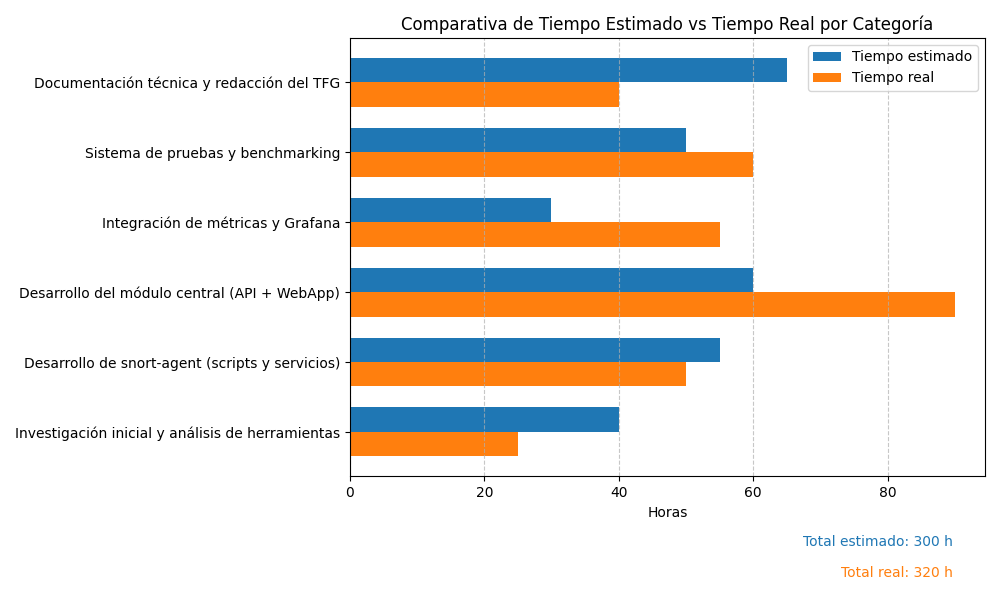
\includegraphics[width=0.8\textwidth]{cronologia/1.png}
	\caption{Cronograma de ejecución del TFG R-SNORT.}
\end{figure}

\begin{figure}[H]
	\centering
	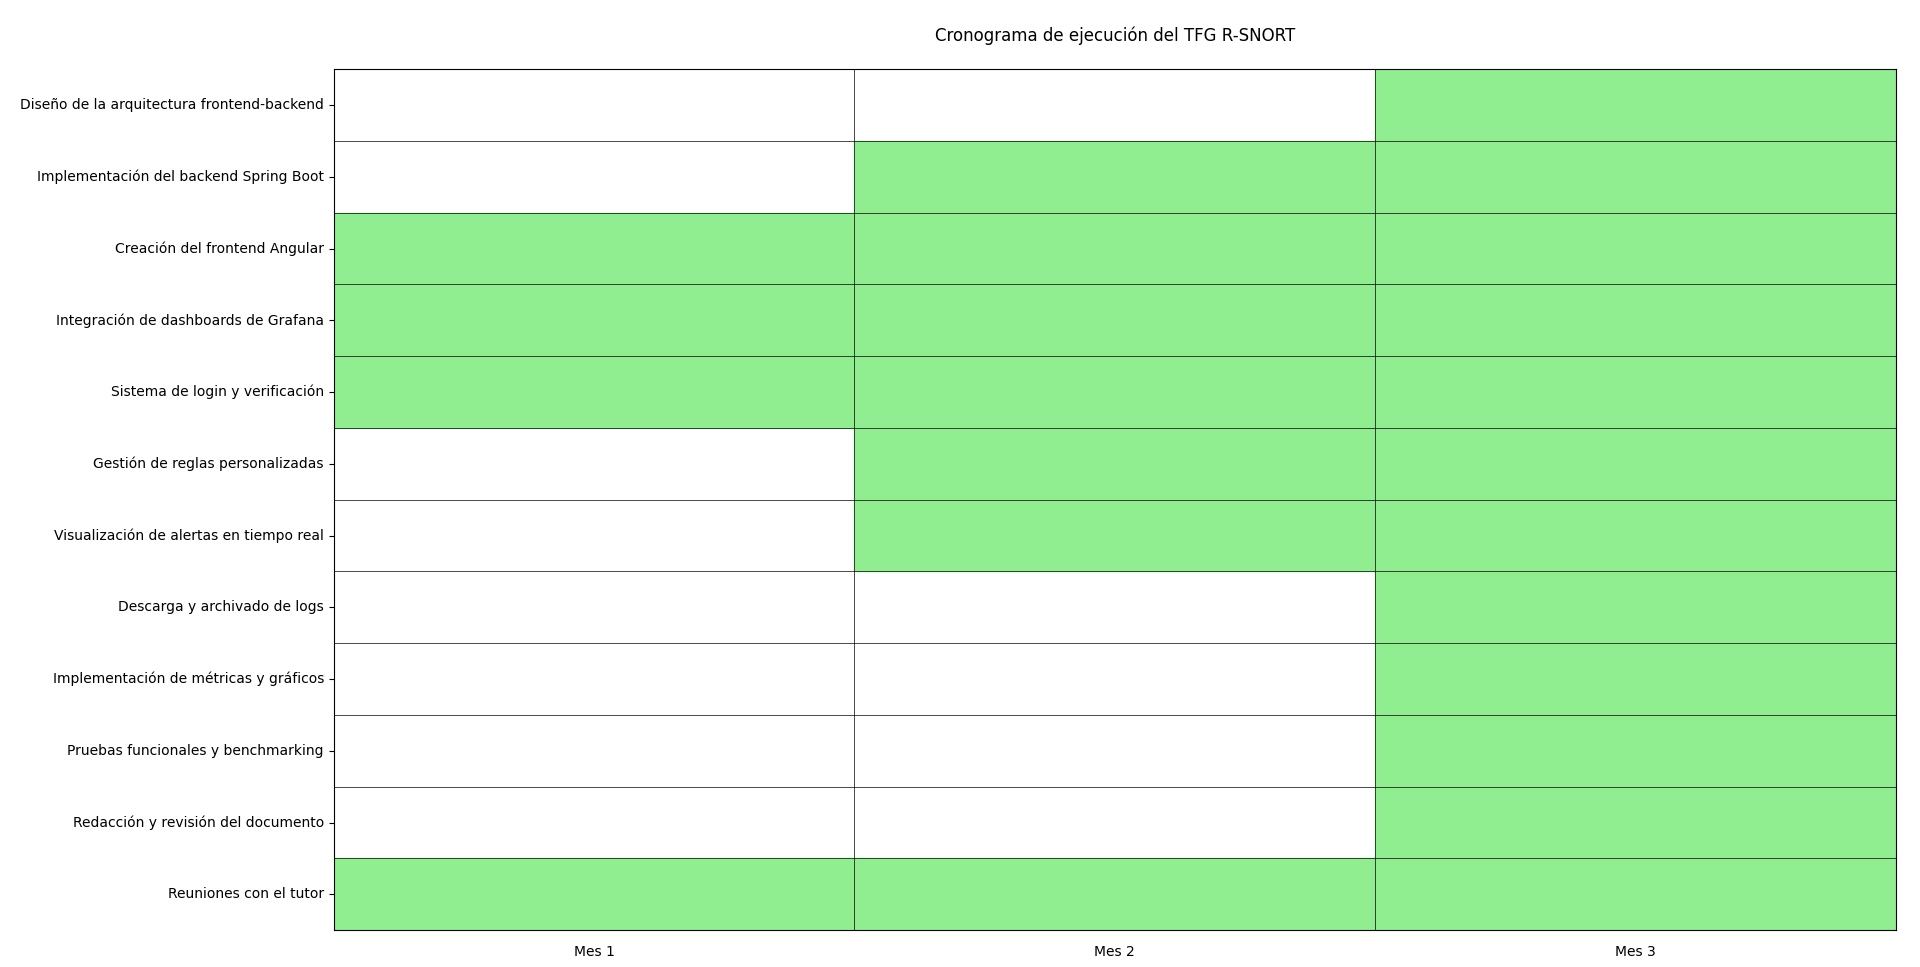
\includegraphics[width=0.8\textwidth]{cronologia/2.png}
	\caption{Comparativa de tiempo estimado vs. tiempo real por categoría.}
\end{figure}

\newpage

En resumen, el desarrollo del TFG R-Snort ha sido un proceso de aprendizaje constante, donde la gestión real del tiempo y la adaptación a problemas inesperados han resultado tan importantes como el propio resultado técnico. Si algo queda para futuros proyectos es que toda planificación es solo una hipótesis inicial: lo realmente valioso es la capacidad de adaptarse, perseverar y terminar el viaje con una solución de calidad.

\section{Estructura y metodología}

El presente documento está estructurado en varios capítulos que permiten seguir el desarrollo del proyecto de manera lógica y progresiva.\newline

\textbf{Introducción, Motivación y Objetivos.} El documento comienza contextualizando la problemática de la ciberseguridad en PYMEs, explicando la motivación personal y profesional detrás del proyecto, así como los objetivos generales y específicos que se han perseguido durante su desarrollo.\newline

\textbf{Fases de la realización y cronograma.} En este apartado se describe cómo se ha organizado y ejecutado el trabajo a lo largo del tiempo, recogiendo las distintas etapas del desarrollo: desde la planificación inicial y el diseño de la arquitectura, pasando por la implementación de los distintos módulos, hasta las fases finales de pruebas, validación y documentación.\newline

\textbf{Capítulo 1: Sistemas de detección de intrusos: Snort y frontends.} Este primer capítulo técnico introduce al lector en el mundo de los sistemas IDS y NIDS, explicando sus conceptos y diferencias principales. Se describe el sistema R-Snort desarrollado en este trabajo, se comparan diferentes frontends existentes para Snort y se analiza el estado del arte de las interfaces web en este ámbito.\newline

\textbf{Capítulo 2: Diseño e implantación de un frontend para R-Snort.} Este capítulo es el núcleo del documento y detalla el proceso de diseño y construcción de la solución propuesta. Se presentan las especificaciones y requisitos del sistema, se describen el entorno hardware y software utilizado, y se profundiza en la arquitectura del sistema, el diseño de la interfaz de usuario y el esquema de la base de datos. Además, se detallan las fases de implementación tanto del backend como del frontend, así como la automatización de la instalación mediante scripts dedicados.\newline

\textbf{Capítulo 3: Caso práctico — utilización del frontend de R-Snort.} En este capítulo se describe cómo se ha desplegado y utilizado el sistema en un entorno realista. Se documentan los pasos de instalación, se muestran capturas de la interfaz y se explican las pruebas funcionales y de rendimiento realizadas, incluyendo la metodología seguida y los resultados obtenidos.\newline

\textbf{Resultados y discusión.} A continuación, se presentan y analizan los resultados obtenidos tras la validación del sistema.\newline

\textbf{Conclusiones y trabajo futuro.} Para finalizar se señala la relevancia práctica de la solución, así como recomendaciones para mejorar o adaptar el sistema en adelante.\newline

\textbf{Bibliografía y anexos.} El documento se cierra con un compendio de referencias bibliográficas y anexos que sirven de manual rápido de la plataforma y de repositorio de recursos prácticos relacionados con el desarrollo, la instalación y la utilización de R-Snort.\newline

En conjunto, la estructura del documento está pensada para que el lector pueda seguir el recorrido completo del proyecto.


\setcounter{secnumdepth}{2} 

\clearpage
\null
\thispagestyle{empty}
\newpage
\chapter{Sistemas de detección de intrusos: Snort y frontends}

\section{IDS / NIDS}

Un \textit{Intrusion Detection System} (IDS), o sistema de detección de intrusos, es una herramienta de seguridad cuya función principal es identificar accesos no autorizados o comportamientos anómalos en un sistema o red informática \cite{wikiNIDS}. Estos sistemas analizan los eventos de la red o del host en tiempo real buscando patrones que puedan indicar amenazas, como ataques de denegación de servicio, escaneos de puertos o intentos de intrusión \cite{NISTSP80094}. En general, un IDS no actúa directamente sobre el tráfico; se limita a monitorizar y generar alertas para notificar a los administradores cuando detecta actividades sospechosas o violaciones a las políticas de seguridad.\newline

Existen dos grandes categorías de IDS según el ámbito que vigilan: los basados en host (HIDS) y los basados en red (NIDS). Un HIDS se despliega en un equipo específico y analiza los registros (\textit{logs}) y actividades de ese sistema para descubrir intrusiones locales (por ejemplo, modificaciones no autorizadas, accesos indebidos, etc.). Por otro lado, un \textit{Network IDS} o NIDS inspecciona el tráfico de una red completa o segmento de red para detectar amenazas que transitan por ella. El NIDS examina todos los paquetes que atraviesan la red en tiempo real, buscando en ellos patrones o firmas conocidas de ataques (malware, \textit{port scanning}, explotación de vulnerabilidades, etc.) y puede detectar tanto tráfico malicioso entrante como saliente. Debido a su naturaleza pasiva (escucha en modo promiscuo una copia del tráfico), un NIDS no introduce prácticamente latencia ni altera el flujo de datos en la red que vigila.\newline

Es importante distinguir un IDS de un sistema de prevención de intrusos o IPS (\textit{Intrusion Prevention System}). La diferencia es que el IDS opera de forma pasiva (detectando y alertando sobre posibles ataques), mientras que un IPS actúa de forma activa/intervencionista: un IPS posee todas las capacidades de detección de un IDS pero, adicionalmente, puede bloquear o impedir automáticamente el tráfico malicioso una vez identificado \cite{a2secure2019}. En otras palabras, el IDS avisa de una intrusión, pero es el administrador quien debe tomar acciones (por ejemplo, actualizar reglas de cortafuegos o aislar equipos comprometidos); en cambio, un IPS está situado en línea en la red y, al detectar un ataque, puede descartarlo o cortarlo en el momento. Por este motivo, a menudo se habla de sistemas IDPS (detección y prevención) cuando una misma solución combina ambas facetas.\newline

Diversos ejemplos ilustran cada tipo de sistema. En el ámbito de host (HIDS) se pueden citar soluciones como OSSEC, Wazuh o Samhain, que monitorizan archivos de log y actividades de un servidor específico. En el ámbito de red (NIDS), destacan herramientas de código abierto ampliamente utilizadas como Snort, Suricata o Bro/Zeek. En particular, Snort se ha convertido en el estándar de facto con el que se comparan todos los IDS de red desde hace más de dos décadas \cite{SnortBlog2011}. Snort es un NIDS (e IPS) open source que emplea un conjunto actualizado de \textit{reglas} de detección para identificar patrones de tráfico malicioso; cuando un paquete o flujo coincide con alguna firma o criterio definido en sus reglas, Snort genera una alerta que notifica del posible incidente \cite{CiscoSnort3Blog}. Además, Snort puede desplegarse en modo \textit{inline} (en línea) actuando como IPS, de forma que no solo detecte sino que también bloquee aquellos paquetes que violen las reglas de seguridad. Esta versatilidad ha hecho que Snort sea una referencia obligada en IDS de red tanto para uso personal como empresarial, contando con una amplia comunidad que contribuye con reglas, mejoras y soporte.\newline


\section{R-Snort}

R-Snort es la denominación del sistema desarrollado en este proyecto, el cual consiste en una solución integral de monitorización y detección de intrusos basada en Snort 3 sobre hardware de bajo coste (una plataforma Raspberry Pi). En esencia, R-Snort implementa un sensor NIDS autónomo que aprovecha las mejoras de la nueva generación de Snort junto con una interfaz web para la gestión y visualización remota de eventos. A diferencia de un IDS tradicional aislado, R-Snort se concibe de forma modular con componentes que automatizan la recolección de datos, el análisis y la presentación de la información de seguridad, todo ello utilizando únicamente tecnologías abiertas.\newline

El \textbf{núcleo de detección} de R-Snort lo constituye Snort 3 ejecutándose en una Raspberry Pi. Snort 3 (también conocido como Snort++) es una reimplementación modernizada del motor Snort que aporta importantes ventajas técnicas respecto a la rama 2.X. Por ejemplo, Snort 3 fue reescrito en C++ para lograr una base de código más modular y fácil de mantener. Incorpora soporte nativo de multiproceso (hilos) y uso de memoria compartida, permitiendo explotar mejor los procesadores multi-núcleo y ofreciendo mayor rendimiento y escalabilidad en la inspección de tráfico. Asimismo, Snort 3 introduce un sistema flexible de complementos (\textit{plugins}) e integración con el lenguaje Lua (LuaJIT) para extender sus funcionalidades, por ejemplo añadiendo nuevas opciones de reglas o analizadores de protocolos de forma más sencilla que antes. La sintaxis de las reglas de detección también se refinó para hacerlas más concisas y fáciles de escribir, reduciendo partes innecesarias y optimizando la velocidad de evaluación \cite{Sakura2020}. Todas estas mejoras hacen de Snort 3 un motor más adaptable, eficiente y potente para nuestro sistema de detección de intrusos.\newline

En R-Snort, Snort 3 actúa como sensor de red, inspeccionando el tráfico (por ejemplo, mediante una interfaz en modo promiscuo o conectado a un puerto espejo de switch) y generando alertas de intrusión en formato JSON. Dichas alertas son procesadas y almacenadas para su consulta mediante la capa de \textbf{back-end}, que está implementada con un servidor web desarrollado en Spring Boot (framework Java) siguiendo una arquitectura de API REST. Este servidor intermedia entre el sensor y la interfaz de usuario, proporcionando servicios como el registro de alertas en una base de datos, la gestión de las reglas activas, y la exposición de endpoints seguros para que los administradores consulten el estado del sistema o apliquen configuraciones de forma remota.\newline

La \textbf{interface web} o frontend de R-Snort se ha construido como una \textit{single-page application} moderna utilizando Angular (framework JavaScript/TypeScript). A través de esta webapp, accesible desde cualquier navegador, el usuario puede visualizar en tiempo real las alertas generadas por Snort, revisar estadísticas históricas, filtrar y buscar eventos por múltiples criterios, así como realizar tareas de administración del sensor (activar/desactivar reglas, reiniciar el servicio IDS, cargar actualizaciones, etc.). El diseño frontend se ha orientado a la simplicidad y claridad en la presentación de datos, inspirándose en las mejores prácticas de UX de aplicaciones de monitorización.\newline

Para enriquecer la experiencia de monitorización, R-Snort integra además la plataforma \textbf{Grafana} como herramienta de visualización de datos de seguridad. Grafana es un software open source ampliamente utilizado para construir paneles de control interactivos, y en este proyecto se emplea para generar gráficas y paneles personalizados a partir de los datos de alertas y métricas del IDS. Por ejemplo, se han creado dashboards que muestran el número de alertas por unidad de tiempo, la clasificación de las alertas por severidad o tipo de ataque, e incluso mapas de calor de IP de origen/destino más detectadas. Este enfoque sigue la línea de otras implementaciones de comunidad que utilizan Grafana para visualizar eventos de Snort (a menudo en conjunción con bases de datos de tiempo real como Elasticsearch/Graylog) \cite{GrafanaForum2020}. En R-Snort, Grafana se conecta al almacenamiento de alertas del back-end y permite tener, dentro de la misma solución, una vista gráfica y analítica de la seguridad de la red en tiempo real.\newline

\begin{figure}[hbtp]
	\centering
	\begin{subfigure}[b]{0.48\textwidth}
		\centering
		
\includegraphics[width=\textwidth]{documento/16.png}
		\caption{Logo de Grafana-Labs.}
		\label{fig:grafana-logo}
	\end{subfigure}
	\hfill
	\begin{subfigure}[b]{0.48\textwidth}
		\centering
		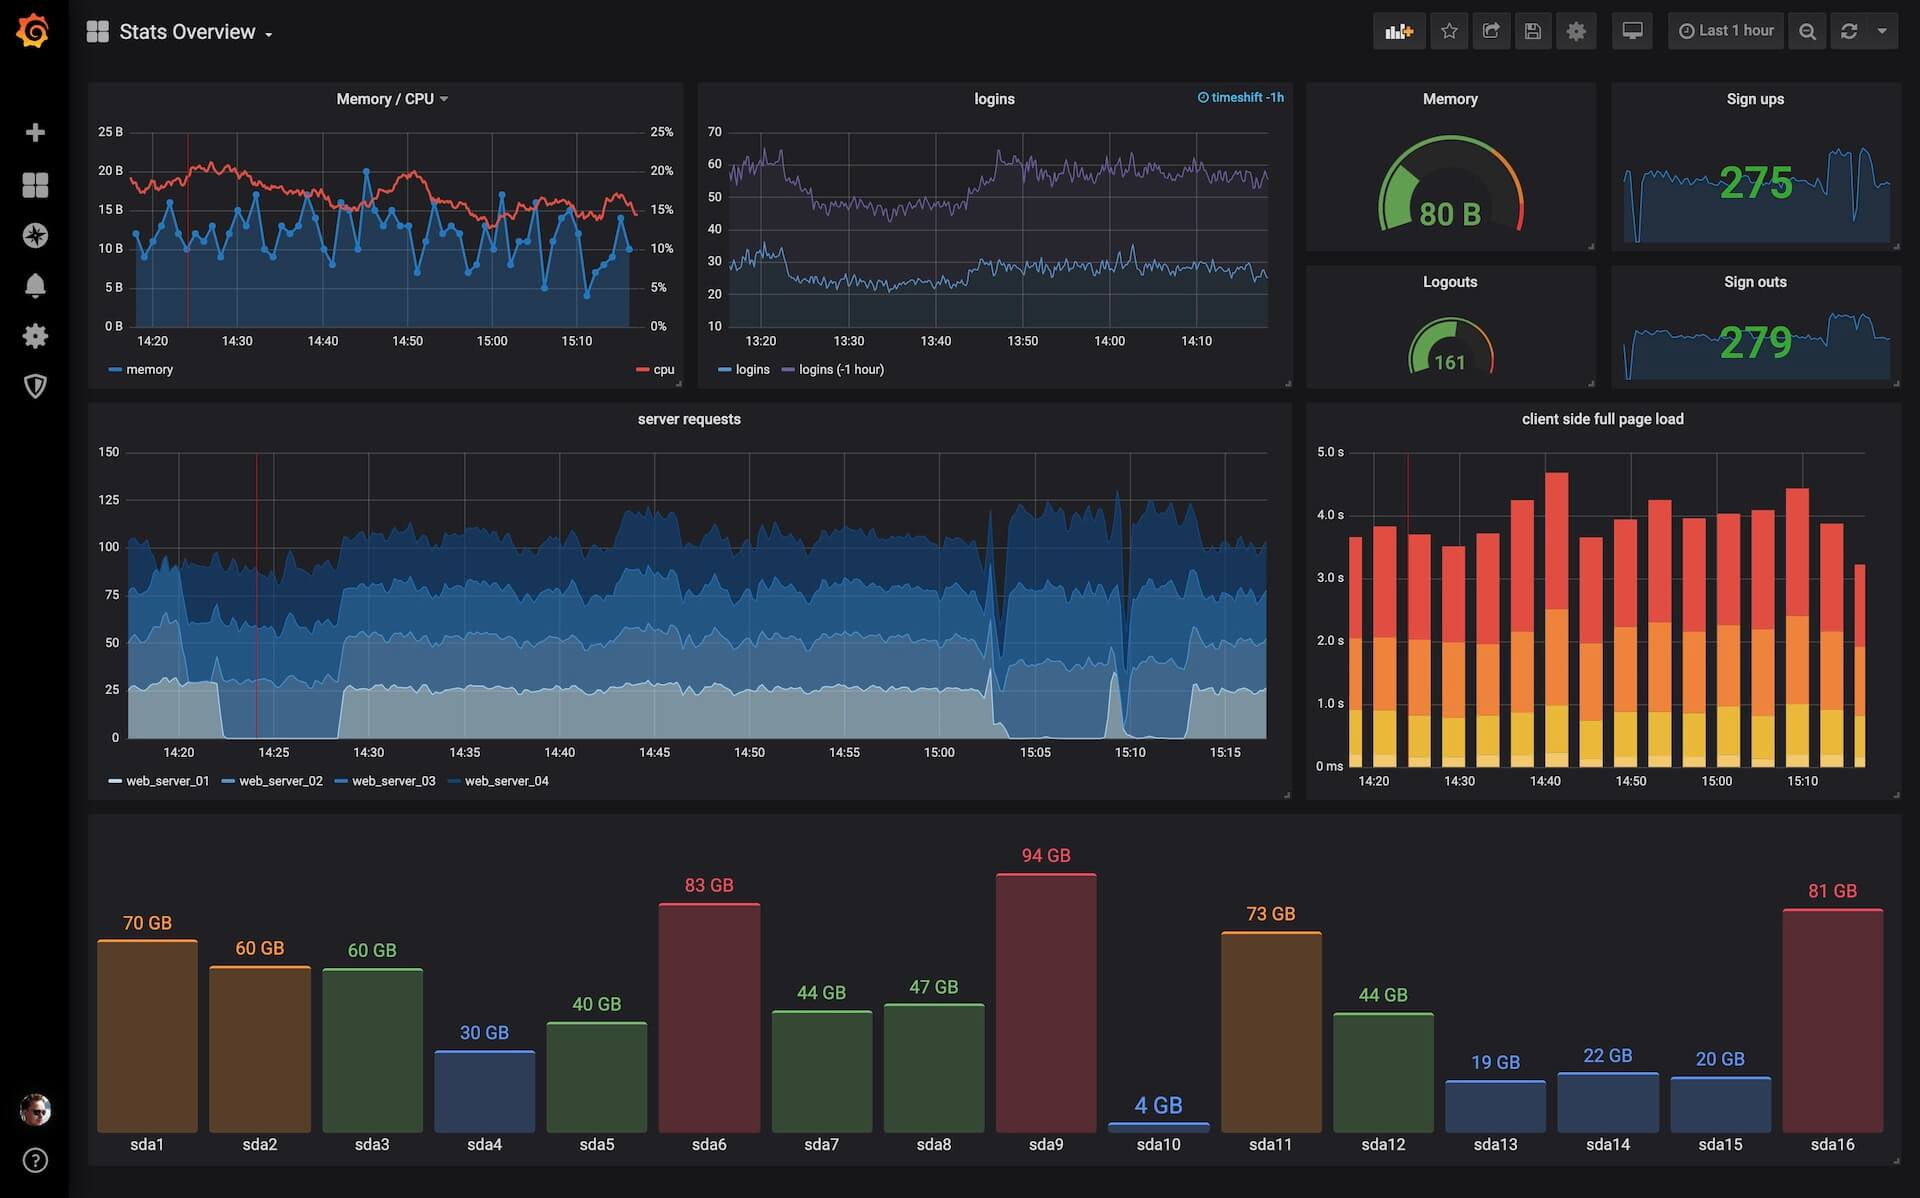
\includegraphics[width=\textwidth]{documento/17.png}
		\caption{Ejemplo de posible dashboard de Grafana.}
		\label{fig:ejemplo-grafana}
	\end{subfigure}
	% \caption{Ejemplo de comparación o conjunto de recursos relacionados con Grafana.} % Solo si quieres un caption global
\end{figure}


En conjunto, R-Snort supone una propuesta de IDS/NIDS completo de bajo coste y código abierto. Combina el potente motor de detección de Snort 3 (sensor) con un ecosistema web moderno (Spring Boot/Angular en el servidor y cliente) y herramientas de visualización profesionales (Grafana) para proporcionar a pequeñas y medianas empresas una plataforma accesible para proteger sus redes. Toda la solución se despliega sobre hardware económico (una Raspberry Pi como nodo sensor), lo que reduce la barrera de entrada en términos de inversión. Pese a su sencillez de despliegue, el sistema mantiene un enfoque modular y escalable: cada componente (detección, almacenamiento, visualización, gestión) está desacoplado, permitiendo en el futuro reemplazar o ampliar funcionalidades (por ejemplo, agregar más sensores en varias ubicaciones reportando al mismo back-end, o incorporar nuevas fuentes de datos de seguridad). En resumen, R-Snort demuestra cómo es posible aprovechar tecnologías abiertas actuales para construir un IDS integrado, manejable vía web y orientado a entornos con recursos limitados, sin incurrir en los altos costes ni complejidad de soluciones comerciales tradicionales.

\begin{figure}[hbtp]
	\centering
	
\includegraphics[width=0.2\textwidth]{logo.png}
	\caption{Logo proyecto R-Snort.}
	\label{fig:logo-rsnort}
\end{figure}

\section{Frontends más utilizados de Snort}

A lo largo de la evolución de Snort han surgido múltiples aplicaciones frontend para facilitar la gestión y análisis de las alertas generadas por este IDS. Estos frontends web proveen consolas gráficas donde los eventos de Snort pueden visualizarse, filtrarse y reportarse de forma más amigable que mediante los logs en texto plano. A continuación se describen algunos de los frontends históricos más populares asociados a Snort –como Snorby, BASE, Aanval, Sguil o Snort Report– incluyendo sus características principales, enfoques y limitaciones, para luego comparar sus conceptos con la propuesta de nuestro R-Snort.\newline

\textbf{BASE (Basic Analysis and Security Engine)} es uno de los frontales web clásicos para Snort. Nació como una continuación del proyecto anterior ACID (\textit{Analysis Console for Intrusion Databases}), el cual fue un pionero en proveer una interfaz web para consultar las alertas registradas por Snort en una base de datos. ACID, desarrollado a inicios de los 2000, quedó discontinuado alrededor de 2003 \cite{SnorbyHelpnet2010}, pero BASE retomó su código y lo mejoró, añadiendo nuevas funciones y compatibilidad con múltiples idiomas. Al igual que ACID, BASE está escrito en PHP y se apoya típicamente en un stack LAMP (Linux-Apache-MySQL-PHP): Snort vuelca las alertas en una base de datos relacional (por ejemplo MySQL) –usando para ello complementos como Barnyard2– y BASE ofrece consultas, gráficos básicos y gestión de alertas desde una página web dinámica. Durante muchos años, BASE fue la interfaz preferida por la comunidad, llegando a superar las 200.000 descargas \cite{base-sourceforge}. Entre sus fortalezas estaban la simplicidad de despliegue y su funcionalidad probada para navegación y búsqueda en los eventos (permitiendo ordenar por fecha, tipo de ataque, IP, etc., y ver detalles de cada alerta). Como limitaciones, al ser una herramienta concebida hace más de 15 años, su interfaz resulta poco moderna y no ofrece visualizaciones avanzadas; además depende de tecnologías y librerías ya obsoletas, lo que puede dificultar su instalación en entornos actuales. A pesar de planes para rediseñar BASE e incluso cambiar su formato de base de datos, el proyecto perdió ímpetu tras la salida de sus mantenedores originales y su desarrollo activo se ha ralentizado considerablemente.

\begin{figure}[H]
	\centering
	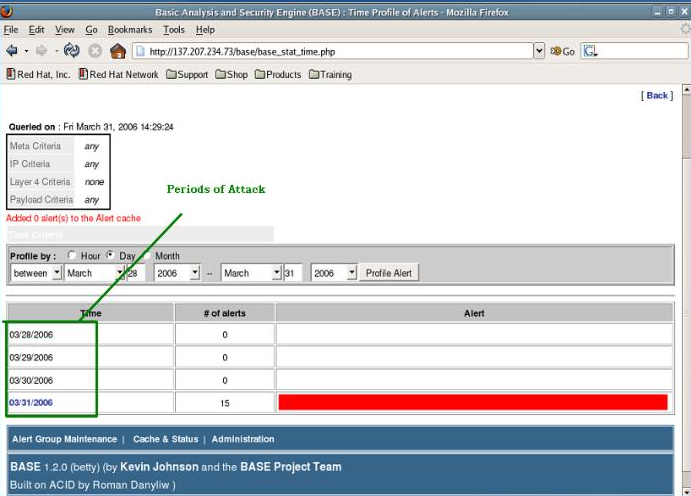
\includegraphics[width=0.5\textwidth]{documento/18.png}
	\caption{Interfaz de BASE.}
	\label{fig:base-interface}
\end{figure}

\textbf{Snort Report} es otra solución veterana, centrada en proporcionar informes rápidos del estado del IDS. Surgido alrededor de 2001, Snort Report se distribuía como un módulo adicional ligero para obtener “instantáneas” de las alertas más recientes y resumir la actividad de Snort en la red \cite{SnortReport2010}. A diferencia de BASE, que brinda múltiples vistas y filtros de análisis forense, Snort Report se enfocaba en la monitorización en tiempo real: presentaba en una pantalla principal un tablero con las alertas actuales (número de eventos, tipo más frecuente, origen de las últimas alarmas, etc.), permitiendo al administrador hacerse una idea inmediata de lo que estaba ocurriendo en su sensor IDS. Era una aplicación sencilla en PHP que leía directamente de la base de datos de Snort o de los archivos de log. Entre sus ventajas estaba la facilidad de uso y la mínima configuración necesaria. Sin embargo, también ofrecía menos profundidad analítica que otras herramientas (no tenía tantas opciones de búsqueda histórica o correlación) y con el tiempo fue quedando relegada en favor de frontends más completos. Aun así, para pequeñas implementaciones Snort Report fue útil por su simplicidad. Con el lanzamiento de Snort 2.x y la aparición de otros dashboards más sofisticados, Snort Report dejó de actualizarse regularmente y hoy en día se considera descontinuado.

\begin{figure}[H]
	\centering
	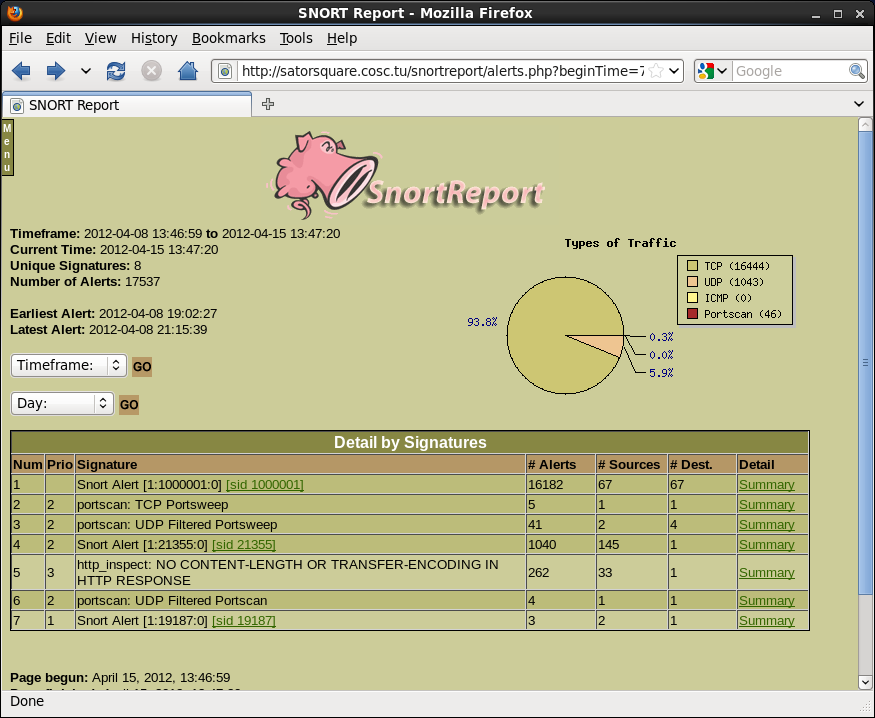
\includegraphics[width=0.6\textwidth]{documento/19.png}
	\caption{Interfaz de Snort Report.}
	\label{fig:snort-report}
\end{figure}

\textbf{Aanval} representa una aproximación distinta, orientada a entornos empresariales que buscaban una solución más completa de tipo SIEM integrando a Snort. Es un producto comercial (desarrollado por Tactical FLEX, Inc.) que desde 2003 ha ofrecido soporte para recoger y correlacionar eventos de Snort, Suricata y fuentes de logs generales (syslog) en una plataforma unificada \cite{AanvalWiki}. Aanval se caracteriza por una interfaz web propietaria bastante pulida, con dashboards personalizables, mapas de topologías, alertas en tiempo real y gestión centralizada de múltiples sensores Snort. A lo largo de sus numerosas versiones, ha incorporado funcionalidades avanzadas como: clasificación de eventos por categorías de ataque, generación de informes ejecutivos, alertamiento vía correo/SMS, e integración con herramientas externas (por ejemplo, ticketing de incidentes). En esencia, Aanval va más allá de un simple visor de alertas y se posiciona como un centro de operaciones de seguridad (\textit{Security Operations Center} simplificado) para quienes despliegan Snort. Entre sus fortalezas está la robustez y amplitud de características, así como su continuidad en el tiempo (es uno de los frontends para Snort con más larga trayectoria, con mantenimiento activo por más de 15 años). Su principal desventaja, desde la perspectiva de nuestro proyecto, es que no es software libre; si bien tuvo versiones gratuitas limitadas, la versión completa de Aanval es de pago, lo que supone una barrera para PYMEs con presupuesto reducido. Asimismo, su enfoque todo-en-uno puede resultar complejo de desplegar en escenarios muy pequeños. No obstante, conceptualmente Aanval demuestra cómo una interfaz web puede escalar para administrar múltiples sensores Snort y agregar inteligencia de seguridad a partir de sus alertas.

\begin{figure}[H]
	\centering
	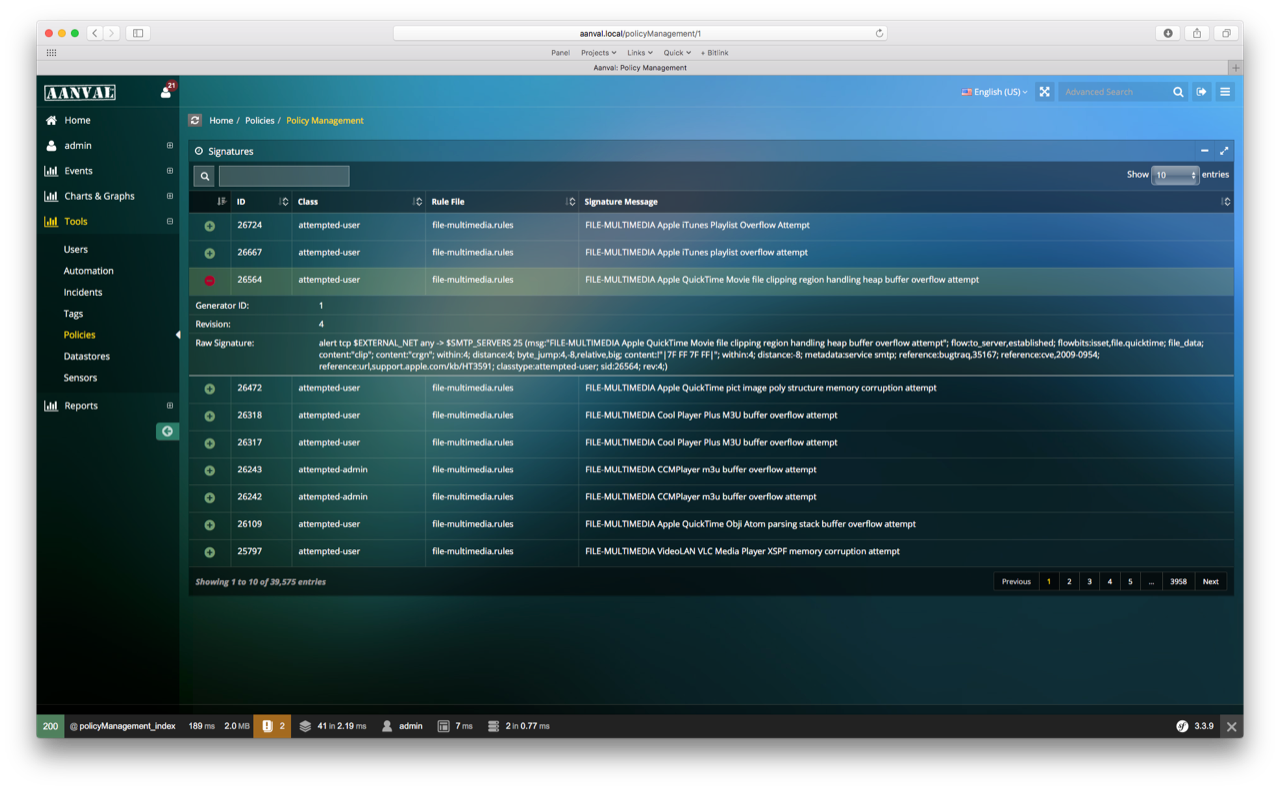
\includegraphics[width=0.6\textwidth]{documento/20.png}
	\caption{Interfaz de Aanval.}
	\label{fig:aanval}
\end{figure}


\textbf{Sguil} (pronunciado \textit{“esquil”}) es otro frontend ampliamente reconocido, aunque su filosofía y arquitectura difieren notablemente de las opciones antes mencionadas. Sguil nació alrededor de 2004 impulsado por Bamm Visscher como parte del paradigma de \textit{Network Security Monitoring} (NSM). A diferencia de BASE o Snorby, que son aplicaciones web puras, Sguil es una solución cliente-servidor pesada escrita en Tcl/Tk que provee una consola para analistas de seguridad. Consta de tres componentes principales: sensores (por ejemplo Snort ejecutándose en modo sensor), un servidor central que recopila eventos, y uno o varios clientes GUI que los analistas utilizan para conectarse y revisar los datos \cite{sectoolsSguil}. Sguil se distingue por proporcionar acceso a información muy detallada: su interfaz gráfica muestra los eventos de Snort en tiempo real (pestaña de \textit{RealTime Events}), y permite al analista profundizar en cada alerta consultando datos de sesión (conexiones relacionadas) e incluso ver las capturas completas de los paquetes asociados al evento, gracias a que integra un sistema de captura continua de tráfico. En esencia, Sguil no solo alerta de un posible ataque, sino que ofrece las evidencias crudas para que un analista las verifique (por ejemplo, reconstruir la sesión TCP o examinar la carga útil del paquete sospechoso). Esto convierte a Sguil en una potente herramienta de análisis e investigación de intrusiones. Muchos administradores empezaban usando BASE para lo básico y luego migraban a Sguil cuando necesitaban capacidades forenses más avanzadas. Sin embargo, toda esta funcionalidad tenía contrapartidas: la aplicación, al estar escrita en Tcl/Tk, resulta menos accesible (no es web, requiere instalar el cliente gráfico) y su usabilidad es más tosca en comparación con las soluciones web modernas. Sguil está muy enfocada al especialista en seguridad, por lo que su curva de aprendizaje es mayor y su interfaz es densa en información técnica. Pese a ello, marcó un hito en cuanto a profundidad de datos disponibles para un IDS y sentó las bases de suites NSM actuales (como Security Onion, que integra Sguil/Squert). Cabe mencionar que existieron frontends web complementarios a Sguil, como Squert, que ofrecían en navegador una vista simplificada de los datos de Sguil, pero incluso estos han ido quedando obsoletos con el tiempo. En resumen, Sguil ofreció una aproximación de “análisis total” del tráfico en torno a Snort, sacrificando la estética y simplicidad a cambio de capacidades analíticas únicas en su momento.\newline

\begin{figure}[H]
	\centering
	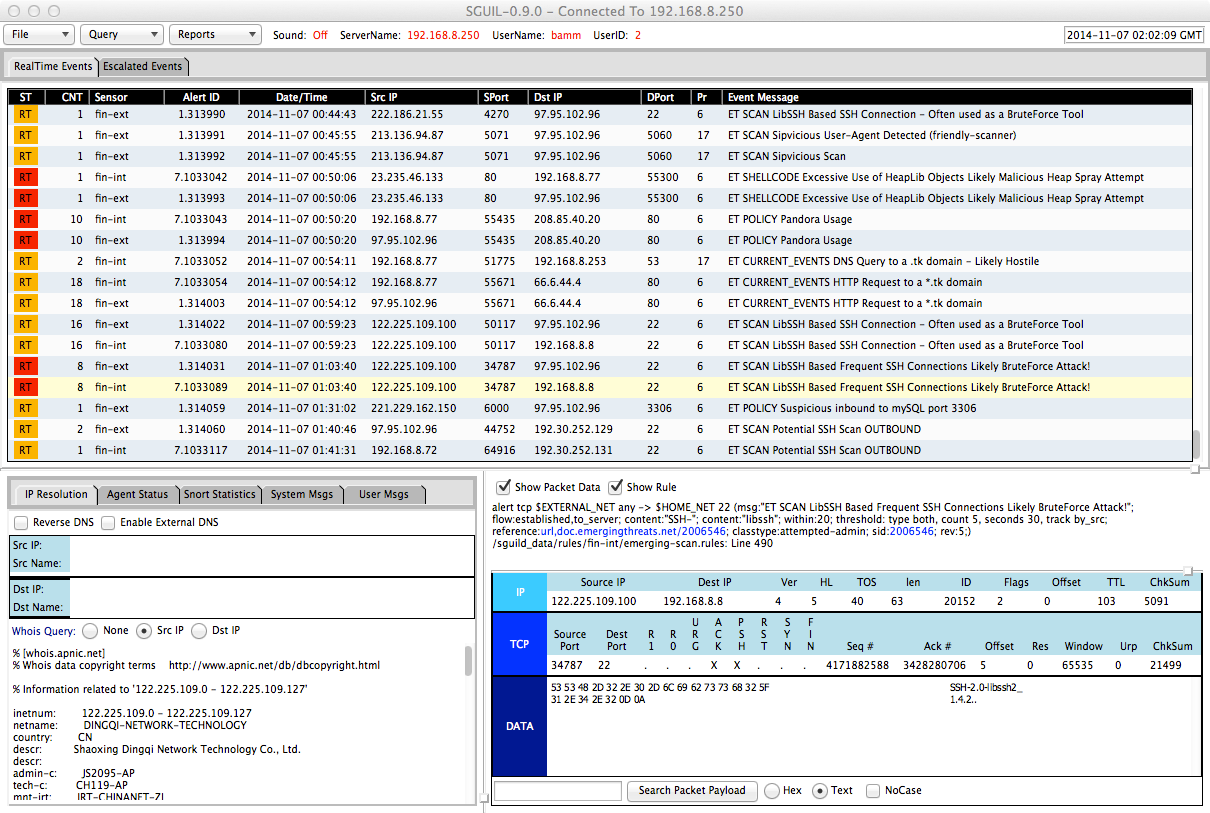
\includegraphics[width=0.6\textwidth]{documento/21.png}
	\caption{Interfaz de Sguil.}
	\label{fig:sguil}
\end{figure}

\textbf{Snorby} es uno de los frontends para Snort más destacables de la década de 2010, pues supuso un intento de modernizar la experiencia de usuario en la gestión de alertas IDS. Presentado originalmente en 2010, Snorby es una aplicación web desarrollada en Ruby on Rails que enfatizaba la interfaz gráfica elegante y la facilidad de uso. Sus principios fundamentales eran la simplicidad y la potencia: el objetivo declarado del proyecto Snorby fue crear una herramienta abierta, gratuita y altamente competitiva para monitorización de redes, dirigida tanto a entornos empresariales como a usuarios particulares \cite{SnorbyHelpnet2010}. A nivel funcional, Snorby retomó muchas características conocidas de BASE (consultas a la base de datos de Snort, filtros por protocolos, exportación de alertas a CSV/PDF, etc.) pero añadiendo numerosas mejoras. Entre las funcionalidades que incorporó estaban: un panel de inicio con métricas y gráficas de las alertas (\textit{dashboard} dinámico), generación automática de informes diarios, semanales y mensuales enviados por correo, sistema de comentarios y anotaciones colaborativas en cada evento (útil para trabajo en equipo), categorización personalizada de la severidad de alertas, y actualizaciones en tiempo real de nuevas alarmas vía AJAX (sin refrescar la página). Incluso ofreció integración con captura de paquetes a través de OpenFPC y aplicaciones móviles (desarrollaron un cliente para iOS). Todo ello con una estética web 2.0 atractiva: gráficos interactivos, uso intensivo de HTML5/CSS3, y una experiencia similar a aplicaciones modernas. Snorby fue considerado durante un tiempo el sucesor natural de BASE en entornos donde no se requería la profundidad de Sguil. Otra ventaja fue la facilidad de despliegue relativamente alta para la época, proporcionándose máquinas virtuales preconfiguradas (Insta-Snorby) para probar el sistema rápidamente. No obstante, Snorby también tuvo limitaciones: su instalación manual podía ser compleja debido a dependencias (particularmente, ciertas gemas de Ruby y librerías como ImageMagick que en distribuciones Linux estables estaban desactualizadas). Además, con el tiempo el proyecto dejó de mantenerse activamente (sus últimas actualizaciones datan de mediados de la década de 2010). Esto, sumado a la aparición de otras soluciones integrales (por ejemplo SIEM completos o el propio Security Onion), hizo que Snorby cayera en desuso recientemente. Aun así, su influencia se nota en el énfasis que puso en la usabilidad del análisis de alertas IDS.

\begin{figure}[H]
	\centering
	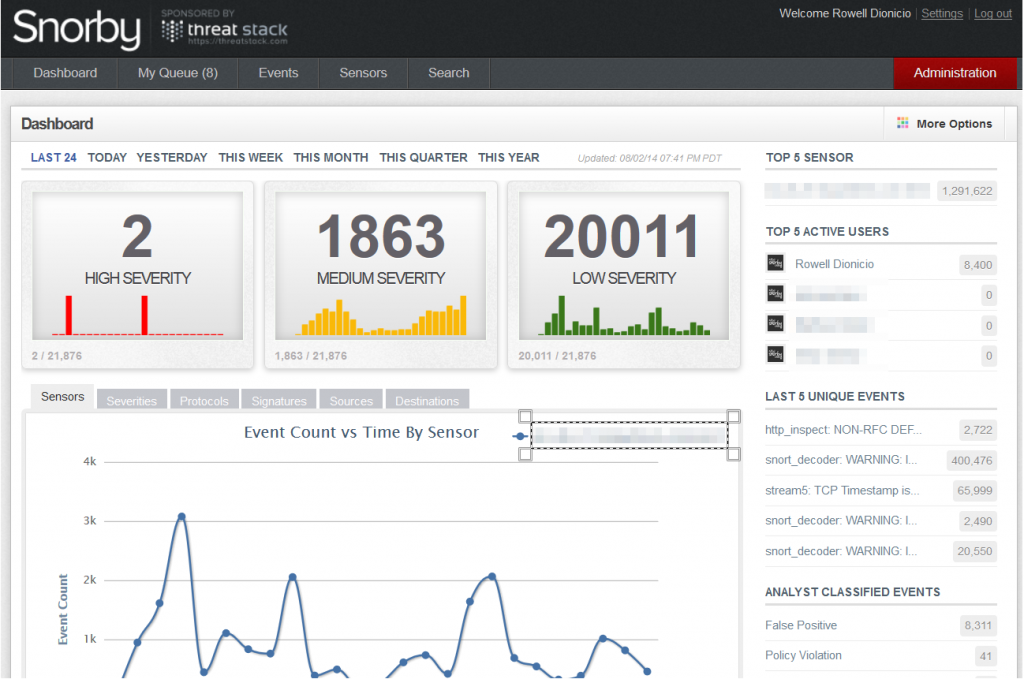
\includegraphics[width=0.6\textwidth]{documento/22.png}
	\caption{Interfaz de Snorby.}
	\label{fig:snorby}
\end{figure}

En perspectiva, cada frontend de Snort mencionado abordó la necesidad de manejar las alertas de intrusión desde un ángulo distinto: unos priorizaron la simplicidad y rapidez (Snort Report, BASE en sus inicios), otros la profundidad de datos (Sguil), otros la estética y facilidad de manejo (Snorby), u ofrecer un ecosistema integral (Aanval). Muchos de estos proyectos, sin embargo, ya no se actualizan o han quedado técnicamente anticuados para los estándares actuales (por ejemplo, ACID/BASE se basaba en PHP5 y Snorby en Rails 3, entornos que hoy presentan problemas de compatibilidad) \cite{StackExchange2011}. La propuesta R-Snort toma inspiración conceptual de estas soluciones previas pero busca aprender de sus limitaciones para ofrecer algo más acorde a los tiempos actuales. En particular, R-Snort comparte con Snorby la filosofía de una interfaz web amigable y orientada al usuario general, donde la información importante esté fácilmente disponible sin mucha complejidad. Del mismo modo que Snorby perseguía “simplicidad y poder”, nuestra aplicación web Angular pretende ser intuitiva pero sin sacrificar funcionalidades clave (por ejemplo, R-Snort permite comentar o marcar eventos, de forma similar al enfoque colaborativo que introdujo Snorby). Por otro lado, recogemos la idea de Sguil de tener una arquitectura modular con sensores dedicados y un servidor central que consolida eventos \cite{sectoolsSguil}; no en vano, R-Snort implementa su sensor Snort en Raspberry Pi y envía las alertas a un servidor web central para su almacenamiento y análisis, emulando en pequeña escala el esquema sensor-servidor-cliente de Sguil (aunque reemplazando el pesado cliente Tcl por una ligera aplicación web). Además, R-Snort brinda cierta capacidad de inspección de datos más allá de la alerta básica integrando Grafana para visualizaciones; esto se inspira en la filosofía NSM de proveer contexto adicional al analista, si bien nuestro proyecto no llega al nivel de captura completa de paquetes que ofrecía Sguil. En comparación con Aanval, R-Snort busca democratizar el acceso a este tipo de herramientas: optamos por tecnologías 100\% open source y asequibles, evitando licencias comerciales o dependencias propietarias, de forma que incluso pequeñas organizaciones puedan desplegarlo sin trabas. Conceptualmente “bebemos” de las lecciones de Aanval en cuanto a consolidar múltiples componentes (detección, base de datos, visualización) en un solo sistema cohesionado, pero simplificando la implementación para que no requiera personal altamente especializado para mantenerlo. En resumen, R-Snort moderniza la idea del frontend de Snort integrando las mejores ideas de proyectos previos (la accesibilidad de Snorby, la arquitectura distribuida de Sguil, la visión general de Snort Report, etc.) y actualizándolas con una arquitectura vigente y orientada a la facilidad de despliegue. El resultado es una solución actualizada que mejora a aquellas históricas en varios aspectos: interfaz web responsiva y actual, instalación sencilla en hardware barato, soporte nativo a Snort 3 (frente a muchas consolas legadas que solo manejaban Snort 2.X), y capacidad de adaptación a las necesidades de monitorización de redes pequeñas con recursos limitados, manteniendo al mismo tiempo un enfoque profesional en la detección de intrusiones.

\section{Comparativa de interfaces web}
Antes de abordar el desarrollo de la interfaz propuesta para R-Snort, es importante analizar las herramientas actuales de monitorización de sistemas de detección de intrusos (IDS) a través de interfaces web. A continuación se presentan tres de las principales soluciones existentes -- la interfaz web de Suricata en \textbf{pfSense}, la consola \textbf{BASE} para Snort y la plataforma \textbf{T-Pot} orientada a Suricata -- describiendo sus características técnicas, ventajas y limitaciones desde el punto de vista técnico y de usabilidad. Este análisis proporciona la base conceptual e inspiración para el diseño de R-Snort, identificando funcionalidades deseables y carencias a evitar en el nuevo sistema.\newline

\subsection{Interfaz web de Suricata en pfSense}
pfSense es un popular cortafuegos de código abierto que puede actuar además como sistema de detección y prevención de intrusiones mediante paquetes adicionales como Snort o Suricata \cite{pfsense}. La interfaz web de administración de pfSense incluye un módulo para Suricata, a través del cual es posible \textbf{configurar el IDS} (por ejemplo, seleccionando reglas, activando la inspección en determinadas interfaces de red, etc.) y \textbf{visualizar las alertas} detectadas. Una vez instalado el paquete de Suricata en pfSense, el administrador accede a una sección dedicada donde se listan todas las alertas registradas por el motor IDS. En la Figura \ref{fig:pfsense-alerts} se muestra un ejemplo de la pantalla de alertas de Suricata en pfSense.\newline

Aunque esta integración facilita la gestión unificada (permitiendo, por ejemplo, \textbf{habilitar o deshabilitar reglas} desde la misma interfaz del cortafuegos), presenta limitaciones importantes en cuanto a usabilidad para el análisis de eventos. En su pestaña de \emph{Alerts}, pfSense muestra el registro completo de alertas en orden cronológico, pero \textbf{no ofrece opciones avanzadas de filtrado o visualización gráfica} de dichos eventos. El analista se encuentra con un listado plano de eventos, lo cual dificulta extraer rápidamente tendencias o detalles específicos cuando el volumen de alertas es elevado. Por ejemplo, no es posible filtrar interactivamente por dirección IP sospechosa, rango de fechas o tipo de alerta desde la interfaz; cualquier filtrado o búsqueda debe realizarse manualmente recorriendo las páginas de resultados. Esta carencia contrasta con herramientas especializadas de monitorización, pero es entendible dado que el enfoque principal de pfSense está en la administración del firewall y la configuración del IDS, más que en el análisis exhaustivo de sus alertas.\newline

Cabe destacar que la interfaz de pfSense sí permite realizar ajustes de \textbf{configuración sobre Suricata} que no están disponibles en otras soluciones de monitorización pura. El administrador puede modificar parámetros del IDS (por ejemplo, modo de detección IDS/IPS, políticas de prevención o gestión de listas de exclusión) directamente desde el entorno web. Esta capacidad de control es una ventaja técnica significativa de pfSense como plataforma integrada. Sin embargo, desde el punto de vista de visualización de datos y experiencia de usuario, la presentación de las alertas es básica: esencialmente tablas de texto sin agregaciones dinámicas ni gráficos interactivos.

\begin{figure}[hbtp]
	\centering
	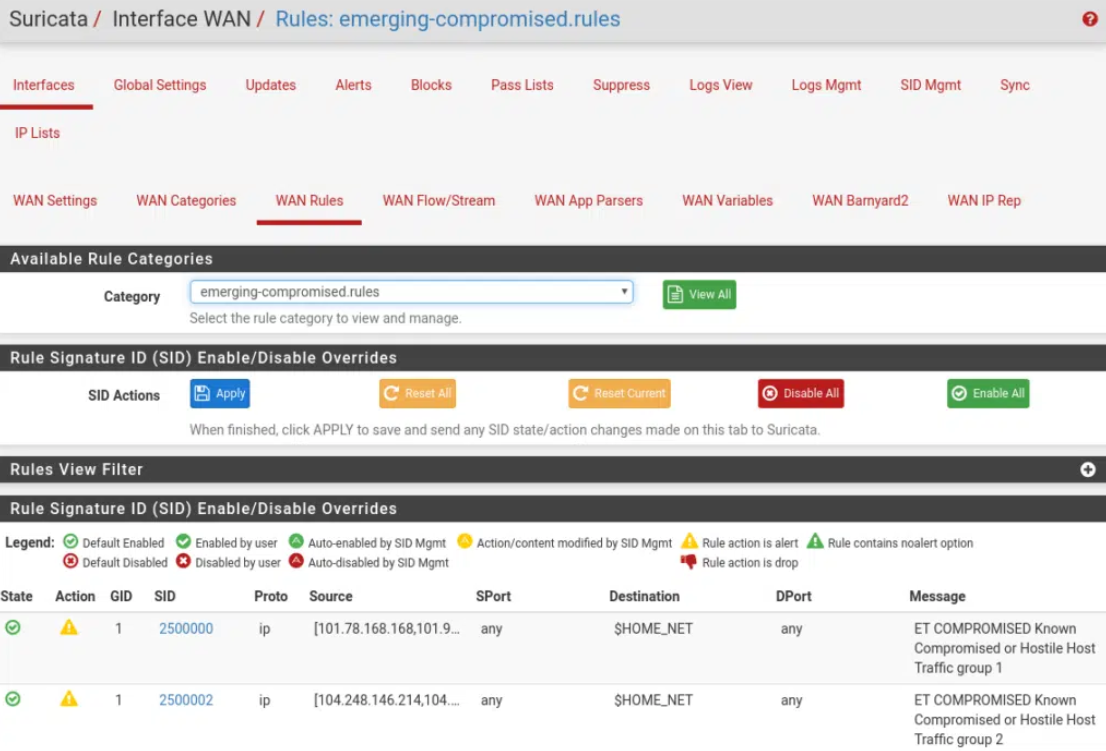
\includegraphics[width=0.9\textwidth]{documento/1.png}
	\caption{Panel de alertas de Suricata en la interfaz web de pfSense.}
	\label{fig:pfsense-alerts}
\end{figure}

\subsection{Interfaz BASE para Snort}
El \emph{Basic Analysis and Security Engine} (BASE) es una de las interfaces web clásicas para la monitorización de Snort. Derivado originalmente del proyecto ACID (Analysis Console for Intrusion Databases), BASE provee un \textbf{frontal web para consultar y analizar las alertas} generadas por un sistema Snort \cite{base}. Este sistema está construido sobre una arquitectura LAMP, empleando un servidor web Apache con páginas PHP que consultan los datos almacenados en una base de datos MySQL. En otras palabras, Snort vuelca sus eventos de alerta en una base de datos y BASE permite explotarlos mediante consultas dinámicas.\newline

A diferencia de pfSense, BASE se centra exclusivamente en el \textbf{análisis de las alertas} y no ofrece funciones para cambiar la configuración del sensor IDS. Su fortaleza radica en las capacidades de 
\textbf{filtrado y agrupación de información} que brinda al analista. La interfaz permite generar consultas predefinidas y personalizadas: por ejemplo, listar las alertas más recientes únicas, obtener las cinco alertas que más se repiten, o visualizar las direcciones IP origen y destino más frecuentes en los registros de intrusiones. La Figura \ref{fig:base-stats} ilustra una de estas visualizaciones, mostrando un resumen de las direcciones IP más detectadas en las alertas. Con estas funciones, BASE facilita identificar patrones de ataque (como hosts atacantes recurrentes o tipos de alertas predominantes) de forma más eficiente que revisando listas planas de eventos.\newline

En términos de \textbf{usabilidad}, la interfaz de BASE, si bien es de corte tradicional, resulta útil para un análisis forense o de seguimiento de incidentes, ya que presenta opciones de búsqueda por múltiples criterios (IP, puerto, fecha, tipo de firma, etc.) y organiza los resultados en formato tabular paginado. No obstante, su diseño es menos interactivo y visual comparado con herramientas modernas: carece de gráficos integrados avanzados o mapas de ataque, y su estética refleja la era en que fue desarrollada (aproximadamente mediados de la década de 2000). Aun así, BASE continúa siendo una referencia en cuanto a funcionalidad de consulta de alertas Snort, proporcionando una base sólida de características sobre la cual se pueden concebir mejoras. Por ejemplo, la idea de incluir filtros por rango temporal o listas de “Top N” alertas en R-Snort toma inspiración directa de este tipo de funcionalidades ya presentes en BASE.

\begin{figure}[hbtp]
	\centering
	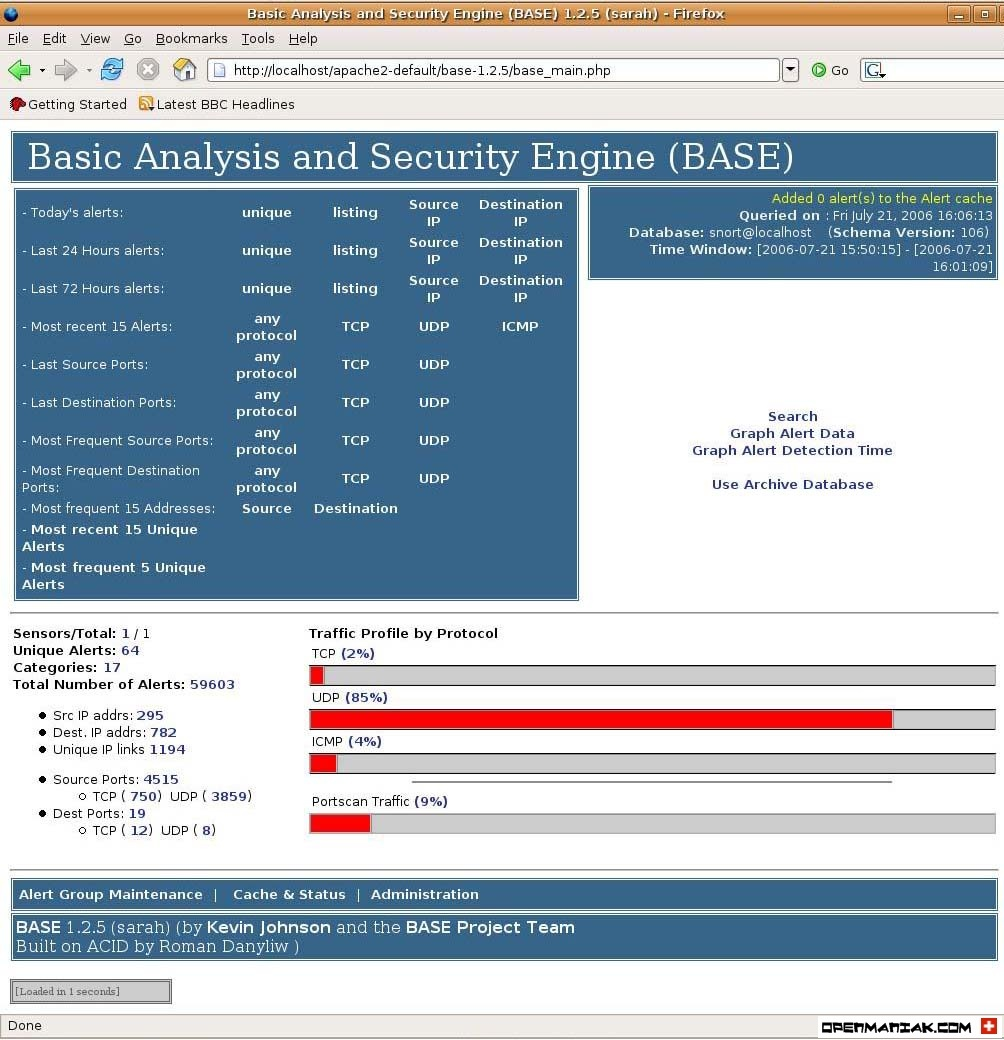
\includegraphics[width=0.85\textwidth]{documento/2.png}
	\caption{Consulta de BASE.}
	\label{fig:base-stats}
\end{figure}

\subsection{Interfaz web de Suricata en T-Pot}
T-Pot es una plataforma integral de \emph{honeypots} mantenida por Telekom Security, que incluye múltiples sensores de seguridad (como Cowrie, Dionaea, conpot, entre otros) y utiliza a Suricata como motor IDS de red. Uno de los atractivos principales de T-Pot es su moderna interfaz de visualización basada en el stack ELK (Elastic Stack). Esta interfaz brinda \textbf{paneles de control gráficos e interactivos} para los datos de alerta. En el caso de Suricata, T-Pot ofrece un panel web integrado (basado en Kibana) que permite analizar las alertas detectadas de forma muy visual. Esta interfaz muestra, por ejemplo, el número total de alertas en un intervalo de tiempo, distribuciones por tipos de amenaza o reglas disparadas, y representaciones como histogramas de eventos en el tiempo y mapas geográficos de las IP de origen de ataques. De hecho, T-Pot soporta "innumerables opciones de visualización" mediante Elastic Stack e incluye mapas de ataque en tiempo real \cite{tpot}. Esto proporciona una experiencia de monitorización más rica y profesional comparada con las interfaces tradicionales.\newline

Al igual que BASE, la consola de Suricata en T-Pot está enfocada en la \textbf{inspección y análisis} de las alertas, sin exponer opciones para reconfigurar el IDS desde la web. Sin embargo, T-Pot supera a BASE en cuanto a presentación: la disponibilidad de gráficos interactivos y estadísticas automáticas facilita la interpretación rápida del estado de seguridad. Además, la interfaz permite aplicar \textbf{filtros dinámicos} sobre los datos: por ejemplo, es posible filtrar las alertas por una dirección IP específica para ver sólo eventos relacionados con esa fuente, o limitar la vista a un rango temporal definido (por ejemplo, las últimas 24 horas o los últimos 5 días) para focalizar el análisis en determinados periodos de actividad. Estas capacidades de filtrado por campo y tiempo aportan una gran flexibilidad al analista, similar a la que se obtiene con herramientas SIEM, y son implementadas de forma transparente gracias a la potencia de Elasticsearch en el backend.\newline

Desde el punto de vista técnico, la solución de T-Pot es más pesada en recursos que las otras dos interfaces: requiere correr contenedores Docker con Elasticsearch, Logstash y Kibana, entre otros componentes, lo cual demanda memoria y almacenamiento significativos. No obstante, este costo se ve compensado por la \textbf{riqueza funcional} que ofrece en monitorización. En entornos donde se despliega T-Pot, normalmente dedicados a investigación de amenazas o vigilancia de \emph{honeypots}, esta interfaz ha demostrado ser muy efectiva para identificar patrones de ataque complejos y correlaciones entre eventos. La Figura \ref{fig:tpot-dashboard} muestra un ejemplo del panel principal de Suricata en T-Pot, donde se aprecian varias visualizaciones simultáneas de los datos de alerta.\newline

\begin{figure}[hbtp]
	\centering
	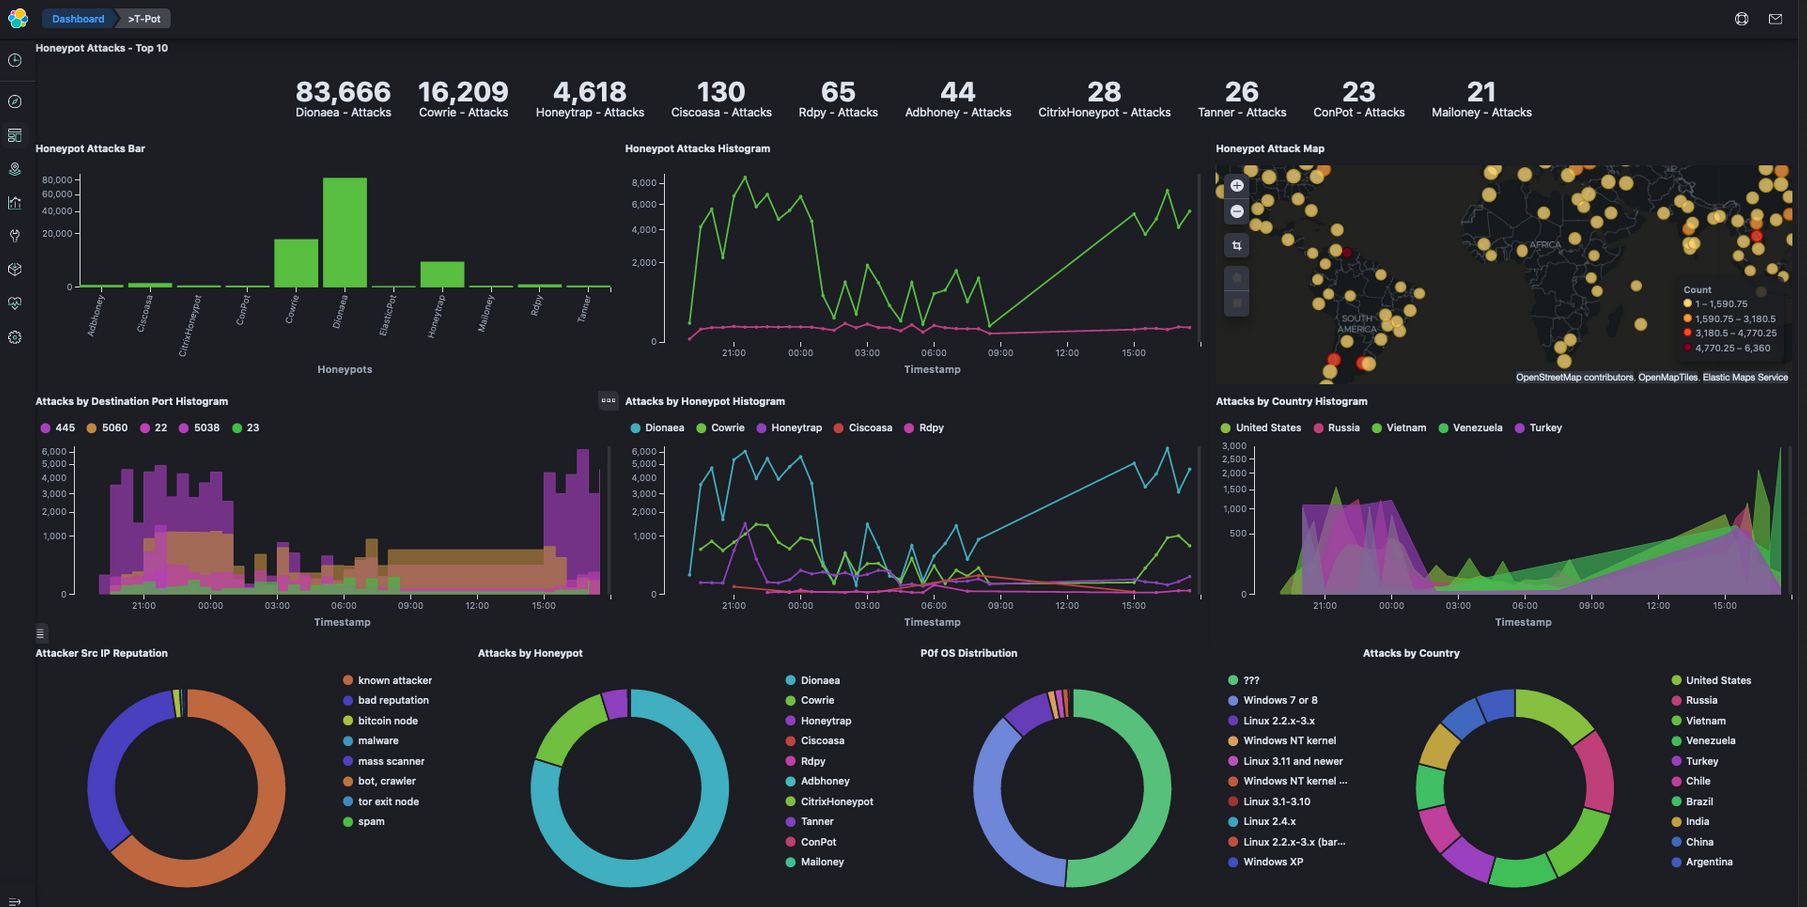
\includegraphics[width=0.9\textwidth]{documento/3.png}
	\caption{Panel principal de Suricata en T-Pot.}
	\label{fig:tpot-dashboard}
\end{figure}

\vspace{1em}
\noindent Una comparativa resumida de las funcionalidades de estas interfaces se presenta en la Tabla \ref{tab:comparativa-interfaces}. Puede observarse que cada solución prioriza un aspecto diferente: pfSense destaca en configurabilidad del IDS, BASE en capacidades de consulta detallada, y T-Pot en visualización avanzada. Estas perspectivas complementarias han sido consideradas en el diseño de R-Snort, buscando integrar lo mejor de cada enfoque. En particular, se procura que R-Snort combine la \textbf{gestión configurable} del sensor (inspirada por pfSense) con \textbf{mecanismos de análisis exhaustivo y visualización intuitiva} (tomando como referentes las fortalezas de BASE y T-Pot, respectivamente).

\begin{table}[hbtp]
	\centering
	\renewcommand{\arraystretch}{1.6}
	\setlength{\tabcolsep}{8pt} % Espaciado horizontal entre columnas
	\begin{tabularx}{\textwidth}{|>{\centering\arraybackslash}X 
			|>{\centering\arraybackslash}X 
			|>{\centering\arraybackslash}X 
			|>{\centering\arraybackslash}X|}
		\hline
		\textbf{Característica} & \textbf{BASE (Snort)} & \textbf{pfSense (Suricata)} & \textbf{T-Pot (Suricata)} \\
		\hline
		Configuración del IDS & No & Sí (completa) & No \\
		\hline
		Filtrado de alertas & Sí (varios criterios) & No & Sí (por IP, tiempo, etc.) \\
		\hline
		Visualización gráfica & Limitada (tablas/listas) & No & Sí (gráficos, mapas, \emph{dashboards}) \\
		\hline
		Tecnología backend & LAMP (Apache/PHP/MySQL) & Integrado en GUI (PHP) & Elastic Stack (Kibana/Elasticsearch) \\
		\hline
		Enfoque principal & Análisis forense de alertas & Gestión de IDS/Firewall & \emph{Honeypot} con monitorización \\
		\hline
	\end{tabularx}
	\caption{Comparativa de funcionalidades de las interfaces web de IDS analizadas.}
	\label{tab:comparativa-interfaces}
\end{table}

\clearpage
\null
\thispagestyle{empty}
\newpage
\chapter{Diseño e implantación de un frontend para R-Snort}

\section{Introducción}
En este capítulo se describe el diseño técnico y la implementación de la interfaz web (\emph{frontend}) y la arquitectura general del sistema \textbf{R-Snort}. Este sistema integra el motor de detección de intrusiones Snort en su versión 3 ejecutándose sobre una placa \textbf{Raspberry Pi 5}, junto con una aplicación web desarrollada en Angular (versión 19) y un servicio backend basado en Spring Boot (Java 17). El objetivo es convertir la instancia de Snort en un \emph{agente} de seguridad monitorizable de forma remota a través de una interfaz web intuitiva y un conjunto de \emph{dashboards} gráficos para alertas y métricas.\newline

R-Snort adopta una arquitectura modular y desacoplada. Por un lado, la Raspberry Pi actúa como \textbf{sensor IDS} ejecutando Snort 3 y exponiendo una \textbf{API REST} mediante el backend Spring Boot; por otro lado, un cliente web Angular permite al usuario interactuar con el sistema (visualizar alertas, configurar parámetros, etc.). Además, se integra la plataforma \textbf{Grafana} para la visualización en tiempo real de las alertas y métricas de rendimiento a través de paneles personalizados. Todos estos componentes se comunican de forma coordinada para proporcionar una solución unificada de monitorización de intrusiones en la red.\newline

Una de las razones para elegir \textbf{Snort 3} como núcleo del sistema es que esta versión ofrece mejoras significativas en eficiencia y escalabilidad respecto a Snort 2.X, incluyendo una arquitectura \emph{multihilo} capaz de aprovechar sistemas multi-núcleo \cite{snort3differences}. Esto resulta en mayor rendimiento y extensibilidad, aspectos clave al desplegar un IDS en hardware limitado como Raspberry Pi. En efecto, Snort 3.0 presenta un diseño renovado y un superconjunto de funcionalidades de Snort 2, logrando mejor eficacia, rendimiento, escalabilidad, usabilidad y extensibilidad. Gracias a esta capacidad multihilo de Snort 3, es posible utilizar todos los núcleos de la Raspberry Pi 5 para el procesamiento de tráfico, aumentando la tasa de análisis de paquetes.\newline

Para la implementación del backend web, se decidió utilizar el framework \textbf{Spring Boot} por su madurez y las facilidades que ofrece (inicio rápido, servidor web embebido, integración con bibliotecas de seguridad, acceso a bases de datos, etc.). Se consideró incluso una alternativa basada en Python como FastAPI, conocida por su alto rendimiento en servicios REST \cite{FastAPI}, pero finalmente Spring Boot fue elegido por su estabilidad y por alinear mejor con los conocimientos y requisitos del proyecto (facilidad de integración con Snort a bajo nivel, uso de JDBC para base de datos, etc.) aunque la herramienta de FastAPI ha servido para la implementación de los agentes individuales. La comunicación entre el frontend Angular y el backend Spring Boot se realiza mediante peticiones HTTP a la API REST, utilizando datos en formato JSON. Para proteger estas comunicaciones y restringir el acceso solo a usuarios autorizados, el sistema implementa autenticación basada en \textbf{JSON Web Tokens (JWT)}. Un JWT es un estándar abierto (RFC 7519) que define un método compacto y seguro de transmitir información entre partes en formato JSON \cite{JWT}, lo que permite verificar la identidad del usuario sin mantener sesiones en el servidor. De este modo, el frontend obtiene un token JWT tras el inicio de sesión y lo incluye en las cabeceras de las peticiones subsecuentes, garantizando un acceso seguro a las funcionalidades de R-Snort.\newline

En la Figura \ref{fig:arquitectura-general} se muestra un diagrama general de la arquitectura de R-Snort. En dicha ilustración se aprecian los principales componentes: la Raspberry Pi ejecuta Snort 3 como agente sensor junto al servicio backend (API REST) que interactúa con Snort y con la base de datos de alertas, el servicio de FAST API se encarga de exponer endpoints para controlar cada sensor; el usuario accede desde un navegador web al frontend Angular, el cual consume la API para presentar información y opciones de configuración; finalmente, Grafana se conecta a la fuente de datos de alertas (base de datos) para ofrecer paneles gráficos actualizables en tiempo real.\newline

\begin{figure}[hbtp]
	\centering
	 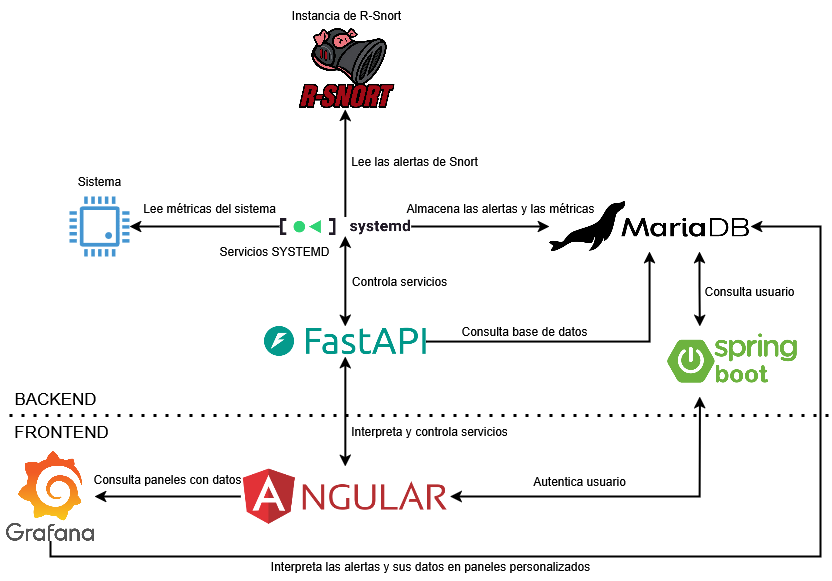
\includegraphics[width=1\textwidth]{documento/5.png}
	\caption{Arquitectura general del sistema R-Snort.}
	\label{fig:arquitectura-general}
\end{figure}

En las secciones siguientes se detallan, primero, las especificaciones y requisitos del sistema (funcionales y técnicos) y, a continuación, el entorno de trabajo utilizado, tanto a nivel de hardware (la plataforma Raspberry Pi empleada como agente de seguridad) como de software (componentes instalados, configuraciones relevantes y herramientas auxiliares). Asimismo, se describe brevemente el entorno de desarrollo y pruebas, donde se aclaran las tecnologías usadas para implementar el frontend y backend, así como la configuración de la red de laboratorio empleada para validar el funcionamiento de R-Snort.\newline

\section{Especificaciones del sistema}
A continuación, se enumeran las principales \textbf{características y requisitos} que se definieron para el sistema R-Snort, abarcando tanto funcionalidades esperadas como consideraciones de diseño e implantación:\newline

\begin{itemize}
	\item \textbf{Motor IDS basado en Snort 3:} El sistema debe emplear Snort en su versión 3 como núcleo de detección de intrusiones. Snort 3 proporciona capacidades mejoradas (p. ej., soporte multihilo, nuevos plugins y sintaxis de reglas mejorada) que incrementan la eficacia y rendimiento de la detección.
	
	\item \textbf{Plataforma hardware accesible:} El IDS ha de poder ejecutarse sobre una Raspberry Pi, aprovechando la portabilidad y bajo coste de este dispositivo. Esto permite desplegar el sensor en entornos domésticos o de pequeña empresa sin requerir hardware dedicado costoso.
	
	\item \textbf{Interfaz web para gestión y monitorización:} Se requiere un frontend amigable, accesible vía navegador, que permita al usuario administrar el sistema y visualizar las alertas detectadas. Este frontend se desarrollará como una \emph{Single Page Application} en Angular, garantizando una experiencia interactiva y fluida.
	
	\item \textbf{Backend REST:} La arquitectura debe seguir un modelo cliente-servidor desacoplado. Para ello, se implementará una API REST en el backend (usando Spring Boot y FAST API) que exponga las funcionalidades necesarias: consulta de alertas, estado de Snort, gestión de configuración, etc. Este backend actúa de intermediario entre Snort, la base de datos y el frontend.
	
	\item \textbf{Visualización de alertas y métricas:} El sistema debe ser capaz de presentar no solo listados de alertas, sino también gráficos y métricas agregadas. Se integrará \textbf{Grafana} para este propósito, configurando \emph{dashboards} que muestren por ejemplo el número de alertas por tipo, tendencias temporales, y métricas de rendimiento (CPU, uso del disco, etc.). Grafana es una plataforma de monitorización y visualización de datos de código abierto ampliamente utilizada en la industria para analítica interactiva \cite{Grafana}.
	
	\item \textbf{Almacenamiento persistente de datos:} Las alertas de intrusión y otros datos relevantes deben almacenarse en una base de datos para permitir su consulta histórica y correlación. Se optó por utilizar una base de datos relacional \textbf{MariaDB} (derivada de MySQL) como repositorio principal de alertas.
	
	\item \textbf{Gestión de reglas y configuración de Snort:} La solución debe facilitar la administración de Snort sin requerir acceder directamente por consola. Esto incluye la posibilidad de agregar reglas IDS (por ejemplo, descargar nuevas reglas de la comunidad o de Snort), eliminar conjuntos de reglas según las necesidades, y ajustar parámetros de configuración de interfaces a través de la web o la API.
	
	\item \textbf{Seguridad y control de acceso:} Dado que la interfaz de gestión expone funcionalidades críticas (ej. ver alertas de seguridad, modificar reglas), es imprescindible restringir el acceso solo a usuarios autorizados. Para ello, se integra un mecanismo de autenticación basado en JWT tal como se mencionó, de forma que cada administrador de R-Snort deba iniciar sesión para obtener un token válido. La comunicación entre frontend y backend debe estar protegida (idealmente usando HTTPS para entornos de producción, evitando la transmisión de credenciales o tokens en texto claro).
	
	\item \textbf{Registro y rotación de \emph{logs}:} Snort genera archivos de registro de alertas que pueden crecer rápidamente. El sistema debe implementar esquemas de \emph{log rotation} para controlar el tamaño de los logs y evitar agotar el espacio en la Raspberry Pi. Por ejemplo, mediante herramientas del sistema (como \texttt{logrotate} en Linux) se rotarán y comprimirán periódicamente los archivos de alertas, manteniendo un histórico reciente y eliminando registros antiguos de forma automatizada.
	
	\item \textbf{Scripts de instalación automatizada:} Para facilitar la puesta en marcha del sistema, se prepararon \emph{scripts} modulares que automatizan la instalación y configuración de los distintos componentes (base de datos MariaDB, entorno Grafana, despliegue del backend Spring Boot, etc.). Cada módulo de instalación puede ejecutarse independientemente, permitiendo por ejemplo instalar solo el agente Snort en una máquina o solo el servidor web en otra, según la arquitectura deseada. Esto refleja la filosofía modular de R-Snort, haciendo posible su adaptación o escalado a futuros despliegues (por ejemplo, múltiples sensores Snort en distintas Raspberry Pi reportando a un servidor central).
	
	\item \textbf{Rendimiento aceptable en hardware limitado:} Se exige que el sistema funcione de manera estable en la Raspberry Pi, atendiendo a sus limitaciones de CPU, memoria y E/S. Esto implica optimizar la configuración de Snort (por ejemplo, cargar únicamente las reglas necesarias, ajustar hilos de procesamiento) y minimizar el consumo de recursos del backend y la base de datos. Las pruebas deben verificar que el IDS puede manejar el tráfico de la red objetivo (típicamente redes domésticas o de oficina pequeña) sin pérdidas de paquetes significativas y con latencia aceptable en la interfaz web.
\end{itemize}

En síntesis, los requisitos anteriores trazan el camino a un sistema completo de detección de intrusos gestionable vía web, construido con tecnologías modernas y enfocado en facilidad de uso, todo ello sobre una plataforma de bajo coste. A continuación, se detalla el entorno de trabajo y la arquitectura de los componentes que dan cumplimiento a estas especificaciones.\newline

\section{Entorno de trabajo}
En esta sección se describe el entorno de hardware y software utilizado para implementar R-Snort, así como el entorno de desarrollo y pruebas empleado durante la construcción del sistema. Se hace énfasis en la configuración de la Raspberry Pi como agente de seguridad, en los componentes de software integrados (Snort 3, complementos y herramientas auxiliares), y en cómo se llevó a cabo el desarrollo del frontend y backend y su validación en un entorno controlado.\newline

\subsection{Hardware: Raspberry Pi como agente de seguridad}
El dispositivo hardware central de la solución es una \textbf{Raspberry Pi}, empleada aquí como un agente de seguridad en la red. En concreto, se utilizó una Raspberry Pi 5, que cuenta con un procesador Quad-core Arm Cortex-A76 a 2,4 GHz y 8 GB LPDDR4X de memoria RAM, capacidades suficientes para ejecutar un IDS ligero junto con un servidor web básico. La Raspberry Pi se eligió por varias razones: es un equipo de bajo coste y tamaño reducido, con un consumo eléctrico mínimo, lo que permite tener un sensor de red siempre activo sin apenas impacto económico; además, su tamaño compacto facilita ubicarla directamente en el entorno de red a monitorizar (por ejemplo, junto al router o switch principal de la organización).\newline

A pesar de sus recursos limitados, la Raspberry Pi ha demostrado ser capaz de albergar sistemas IDS/IPS funcionales en escenarios de pequeña escala. Por ejemplo, existen guías prácticas que muestran cómo convertir una Raspberry Pi en un IDS/IPS completamente funcional capaz de detectar intrusiones en la red. De hecho, la comunidad de seguridad ha validado la viabilidad de esta aproximación, aprovechando la portabilidad y suficiencia de procesamiento que ofrece este microordenador \cite{SecMaster2024}. En nuestro caso, la Pi actúa como un \emph{appliance} de seguridad dedicado: captura el tráfico de la red, ejecuta Snort para analizar dicho tráfico en busca de patrones maliciosos, y envía las alertas generadas a los subsistemas correspondientes (base de datos, interfaz web, dashboards, etc.).\newline

La forma de \textbf{integración en la red} de la Raspberry Pi depende del modo de funcionamiento del IDS. En este proyecto, R-Snort se despliega en modo \emph{pasivo} (IDS puro, no IPS), es decir, la Pi monitoriza el tráfico sin interrumpirlo. Para lograr esto, una práctica común es conectar la interfaz de red de la Pi a un puerto espejo (\emph{mirror/span port}) de un switch, o en su defecto, colocarla en la misma subred que los equipos a vigilar y configurar reglas apropiadas de captura. De esta manera, la Pi recibe copias del tráfico de red pero no introduce latencia ni punto de falla en la comunicación. Alternativamente, si se buscara un modo \emph{inline} (IPS), sería necesario contar con dos interfaces de red en la Raspberry Pi y configurarla como puente; sin embargo, para simplificar la implantación, R-Snort se centra en la monitorización pasiva.\newline

En la Figura \ref{fig:despliegue} se ilustra un posible \textbf{esquema de despliegue} de R-Snort en una red local. La Raspberry Pi está conectada al switch de la red mediante cable Ethernet; el switch está configurado para duplicar el tráfico de los dispositivos hacia el puerto donde se encuentra la Pi, permitiendo que Snort inspeccione los paquetes. El administrador puede acceder al frontend web y a los paneles de Grafana desde un equipo en la misma red (o remotamente vía VPN), conectándose a la dirección IP de la Raspberry Pi. Así, la Pi actúa como nodo de monitorización, analizando el tráfico y reportando alertas sin interferir en la comunicación normal de la red.\newline

\begin{figure}[hbtp]
	\centering
	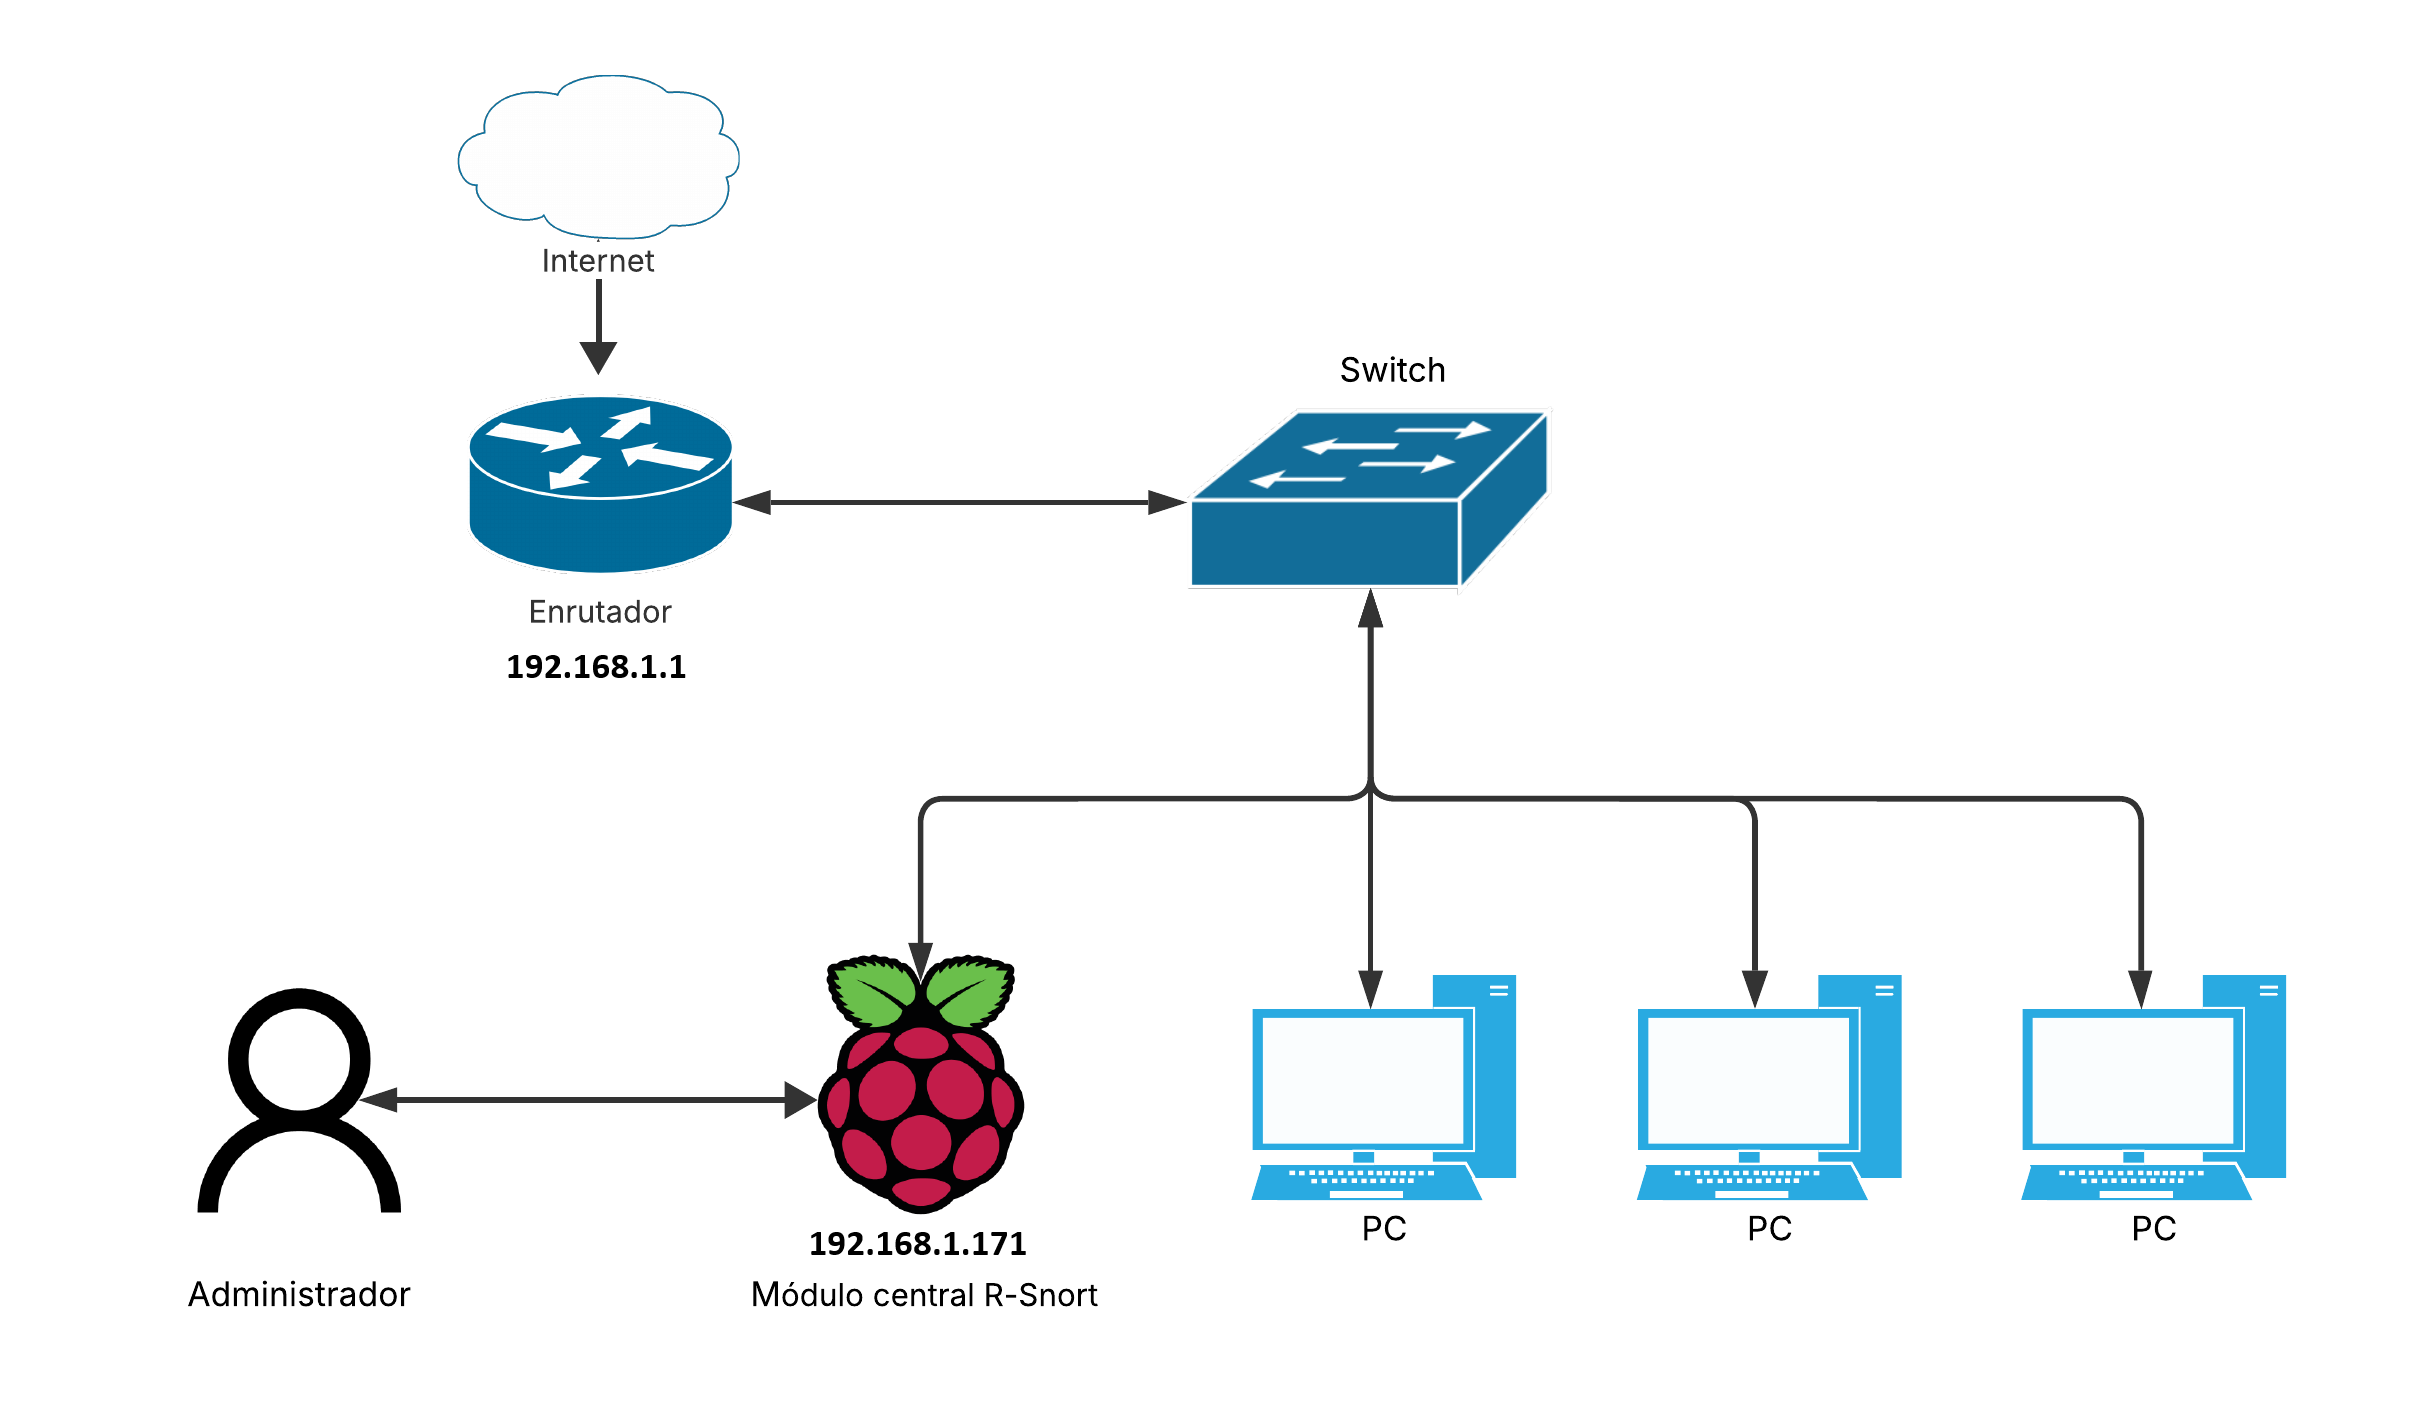
\includegraphics[width=0.8\textwidth]{documento/4.png}
	\caption{Esquema de despliegue de R-Snort en la red local.}
	\label{fig:despliegue}
\end{figure}

En cuanto al \textbf{sistema operativo} utilizado en la Raspberry Pi, se optó por una distribución Linux de 64 bits para garantizar compatibilidad con Snort 3 y un buen aprovechamiento de la memoria. En particular, se empleó Ubuntu Server de 64 bits. Esta elección minimiza la carga de procesos innecesarios y permite dedicar la mayor parte de los recursos al IDS y al servidor web. Todas las interacciones con la Pi (instalación de paquetes, edición de configuraciones, revisión de logs) se realizaron vía acceso remoto SSH, ya que la Pi operaba en modo head-less (sin monitor ni periféricos).\newline

Es importante resaltar que, aunque la Raspberry Pi 5 ofrece un rendimiento notable para su tamaño, sigue estando lejos de un hardware de servidor. Por ello, el volumen de tráfico que puede analizar en tiempo real es limitado. En entornos de alta carga (por ejemplo, redes gigabit con tráfico sostenido muy elevado) es posible que la Pi se vea sobrepasada. Sin embargo, para entornos objetivo de este proyecto (redes domésticas o PYMEs, típicamente con anchos de banda de decenas de Mbps y tráfico intermitente), la capacidad de la Pi es adecuada. Estudios de rendimiento han mostrado que Snort (y herramientas similares como Suricata) corriendo en una Raspberry Pi pueden llegar a inspeccionar del orden de cientos de Mb/s con configuraciones optimizadas \cite{SecMaster2024}, lo cual cubre las necesidades planteadas. En cualquier caso, durante las pruebas se ha monitorizado el uso de CPU, memoria y red de la Pi para asegurar que el sistema operaba dentro de márgenes seguros.\newline

\subsection{Software: Snort 3 y complementos}
A nivel de software, el componente principal es el \textbf{motor IDS Snort 3}. Snort es un sistema de detección de intrusiones de código abierto ampliamente utilizado, basado en análisis de firmas/patrones definidos en reglas. La versión 3 de Snort representa una reimplementación moderna del IDS clásico, aportando una serie de mejoras que resultan beneficiosas para este proyecto. Entre ellas cabe mencionar el soporte multi-hilo (permitiendo procesar paquetes en paralelo), un nuevo lenguaje de reglas más flexible, y la disponibilidad de más de 200 complementos o \emph{plugins} para diversas funcionalidades. Todas estas mejoras conllevan una mayor eficiencia y facilidad de extensión del IDS, factores cruciales al desplegarlo en un entorno limitado pero que puede requerir personalizaciones.\newline

En R-Snort, Snort 3 se configuró en \textbf{modo IDS} (no bloquea tráfico, solo alerta) y se ejecuta como servicio en la Raspberry Pi. Se personalizó el archivo de configuración de Snort (en formato Lua, propio de Snort3) para adaptarlo a la red local monitorizada: se definió la variable \texttt{HOME\_NET} con el rango de IP interno a proteger, se ajustaron los puertos considerados para ciertos protocolos (por ejemplo incluir puertos de servicios comunes en la red local) y se activaron preprocesadores relevantes (como \emph{Stream5} para seguimiento de sesiones TCP, \emph{HTTP Inspect} para analizar tráfico web, etc.). Asimismo, se habilitó la salida de alertas en \textbf{formato JSON}, mediante el uso del \emph{plugin} \texttt{alert\_json}, de modo que cada evento de alerta que genera Snort se registra como una entrada JSON estructurada (conteniendo campos como timestamp, dirección IP de origen y destino, puerto, identificación de la regla que se disparó, mensaje de alerta, etc.). Este formato resulta conveniente para su posterior procesamiento automatizado por otras partes del sistema.\newline

Adicionalmente, se utilizaron ciertos \textbf{complementos de Snort} necesarios para su correcto funcionamiento en Raspberry Pi. En particular, se instaló la librería \textbf{DAQ} (\emph{Data Acquisition}) apropiada para capturar el tráfico de red; en este caso, se usó \texttt{af\_packet} (incluida con Snort 3) que permite leer directamente de la interfaz de red en modo promiscuo con buen rendimiento. También se configuró Snort para que se ejecute con privilegios limitados por seguridad (utilizando el usuario \texttt{snort} y grupo \texttt{snort} creados en el sistema) y se creó un servicio \texttt{systemd} para su lanzamiento automático en el arranque de la Pi.\newline

Otro aspecto importante es la gestión de las \textbf{reglas IDS}. Para este proyecto, se decidió comenzar utilizando las \emph{reglas comunitarias} gratuitas de Snort (Snort Community Rules) y algunas reglas emergentes de Emerging Threats, para disponer de un conjunto base que cubra amenazas comunes. Se implementó un script de actualización que, bajo demanda o de forma programada, descarga las últimas reglas (mediante \emph{oinkcode} si aplica, en el caso de Snort) y actualiza el directorio de reglas de Snort. Así, desde la interfaz de R-Snort, el usuario podría desencadenar la actualización de reglas sin tener que hacerlo manualmente. Aunque herramientas clásicas como \texttt{PulledPork} aún no tienen versión oficial para Snort 3, se logró una funcionalidad similar mediante scripts en Bash que automatizan la descarga y colocación de nuevos archivos de reglas, seguidos de un reinicio suave de Snort para aplicar los cambios. (Ver el complemento de TFG para más detalles).\newline

Además del propio Snort, el sistema incorpora varios \textbf{componentes software complementarios} que, en conjunto, constituyen la solución completa:\newline

\textbf{Backend central en Spring Boot:}
Desarrollado en Java 17 mediante el framework Spring Boot, este módulo no se instala en las Raspberry Pi (agentes), sino que reside en el servidor principal, actuando como centro de control y despliegue del sistema. Su función se limita a gestionar la autenticación, la gestión de usuarios y la coordinación de los distintos agentes de la red. Para ello, expone varios endpoints REST como \texttt{/api/login} (para iniciar sesión mediante credenciales y obtener un token JWT), \texttt{/api/agents} (para listar y registrar agentes disponibles). Un \textbf{agente} en este contexto es una Raspberry Pi con Snort y el software auxiliar instalado, dedicada a monitorizar el tráfico de red local de una ubicación concreta. Cada agente se comunica con el backend central para facilitar la administración remota y permitir que un único punto de control visualice, gestione y configure todos los nodos desplegados.\newline

\textbf{Backend local en cada agente (FastAPI):}
Cada Raspberry Pi funciona de manera autónoma como agente de monitorización, gracias a un backend ligero desarrollado en Python mediante FastAPI, denominado internamente \texttt{fasatpi}. Este componente se instala localmente en cada dispositivo o módulo de R-Snort y es el encargado de proporcionar la información propia del agente a la interfaz web. Expone endpoints REST como \texttt{/alerts}, \texttt{/status}, \texttt{/rules} o \texttt{/logs}, los cuales permiten consultar alertas generadas, comprobar el estado de Snort, gestionar reglas o descargar logs archivados.
Internamente, \texttt{fasatpi} accede a los archivos JSON generados por Snort, así como a la base de datos local MariaDB donde se almacenan las alertas y métricas. Además, implementa acciones sobre el sistema, como reiniciar Snort mediante scripts o comprobar el estado de servicios mediante comandos shell. Gracias a este diseño, cada agente puede funcionar de forma autónoma incluso sin conexión constante al backend central, y ofrece una interfaz clara para que R-Snort WebApp pueda consultar y controlar su estado desde la red.\newline

\textbf{Base de datos MariaDB:} Para persistir las alertas y otros datos, se configuró un servidor de base de datos MariaDB 10.x corriendo en la propia Raspberry Pi. Cada alerta generada por Snort es insertada en una tabla (p. ej. \texttt{alerts}) con campos como timestamp, IP origen, IP destino, puerto, protocolo, SID de la regla, mensaje, etc. Esta inserción se realiza de manera automática: el backend Spring Boot incluye un componente que supervisa la aparición de nuevas entradas en el log JSON de Snort (mediante un hilo que observa el archivo o utilizando mecanismos de notificación del sistema de ficheros) y en cuanto detecta una nueva alerta, la parsea del JSON e inserta los datos en la base MariaDB mediante JDBC. De esta forma, construimos una \textbf{pipelines} de datos desde Snort hacia la base de datos casi en tiempo real. Cabe mencionar que Grafana y el propio frontend consultarán esta base para mostrar la información al usuario.\newline

\textbf{Grafana:} Es la herramienta seleccionada para la visualización gráfica de los datos. Grafana es una aplicación web de monitorización que permite crear paneles interactivos a partir de diversas fuentes de datos (tiempo real, series temporales, etc.) \cite{Grafana}. En R-Snort, se instaló Grafana OSS (código abierto) versión 12 en la Raspberry Pi, aprovechando que existen builds para arquitectura ARM. La instancia de Grafana se configuró para conectarse a la base de datos MariaDB como \emph{data source} utilizando el conector MySQL. De esta forma, se pudieron escribir consultas SQL sobre la tabla de alertas y representar resultados en gráficas. Grafana se ejecuta como un servicio aparte, corriendo en el puerto 3000 de la Raspberry Pi, y la interfaz Angular tiene la opción de embeber ciertos paneles de Grafana mediante iframes o bien el usuario puede acceder directamente al dashboard completo de Grafana para análisis más avanzados. Ambos (frontend propio y Grafana) beben de la misma base de datos de alertas, garantizando consistencia en la información.\newline

\textbf{Rotación de logs y mantenimiento:} A nivel de sistema operativo, se añadieron configuraciones para mantener el sistema funcionando sin intervención manual. En particular, se creó una tarea \texttt{cron} diaria que ejecuta \texttt{logrotate} sobre los archivos de log de Snort (y opcionalmente logs del backend), de modo que cada día se archiva el log del día anterior y se comienza uno nuevo, conservando, por ejemplo, solo 7 días de logs comprimidos. Asimismo, se desarrollaron pequeños scripts de \emph{health-check} que comprueban si el proceso de Snort sigue activo y, si no, intentan reiniciarlo usando \texttt{systemctl}; esto agrega robustez frente a eventuales caídas del IDS. El backend Spring Boot se configuró también como servicio de sistema para iniciarse automáticamente en el arranque (\texttt{systemd service}) y reiniciarse en caso de falla.\newline

En resumen, la Raspberry Pi ejecuta de forma concurrente varios servicios: Snort 3 (detección de intrusos), Spring Boot (API REST y lógica de negocio), FAST API (datos del sistema), MariaDB (almacenamiento de datos) y Grafana (visualización). Gracias a la optimización y a la moderada carga esperada, la Pi es capaz de manejar estos componentes simultáneamente. Cada uno cumple un rol específico pero se complementan para brindar la funcionalidad global de R-Snort. El diseño modular permite incluso que, de ser necesario, alguno de estos componentes pudiera desplazarse a otro equipo (por ejemplo, usar un servidor externo para Grafana o la base de datos) sin grandes cambios, evidenciando la flexibilidad de la arquitectura planteada.\newline

\subsection{Entorno de desarrollo}
El desarrollo del frontend y backend de R-Snort se llevó a cabo utilizando herramientas modernas y siguiendo buenas prácticas para garantizar la calidad del software. Para la parte de \textbf{frontend Angular}, se empleó \textbf{TypeScript} como lenguaje de programación y el \emph{framework} Angular en su versión 19. La estructura del proyecto Angular se inicializó con \texttt{angular-cli}, organizando los componentes, servicios y rutas de la aplicación de forma modular. Durante la implementación, se hizo uso de un conjunto de librerías de interfaz comunes (por ejemplo, Angular Material) para agilizar la construcción de elementos UI como tablas, diálogos modales y gráficos simples. El entorno de desarrollo incluyó herramientas como \textbf{Visual Studio Code} como editor principal y el servidor de desarrollo de Angular (\texttt{ng serve}) que permitía ver los cambios en vivo en el navegador durante la codificación. Para el manejo de versiones del código se utilizó Git, lo cual facilitó llevar un control de cambios y colaborar en caso de integración de diferentes partes.\newline

En cuanto al \textbf{backend Spring Boot}, se utilizó el \emph{stack} típico de Spring: Spring MVC para la creación de controladores REST, Spring Data JPA para la capa de persistencia con MariaDB (definiendo entidades JPA que representan las alertas, etc.), y Spring Security para implementar la capa de autenticación JWT. El proyecto se configuró con \texttt{Maven} como gestor de dependencias. Durante el desarrollo, se probaban los endpoints localmente en un equipo de escritorio antes de desplegarlos en la Raspberry Pi, usando herramientas como \textbf{Postman} para verificar las respuestas JSON de la API. Una vez validados, el backend se compilaba en un \emph{JAR ejecutable} (\texttt{spring-boot fat jar}) y se transfería a la Pi para su ejecución en producción. La Pi cuenta con OpenJDK 17 instalado para correr la aplicación Java.\newline

Para asegurar la \textbf{integración del frontend con el backend}, se habilitó \textbf{CORS} (Cross-Origin Resource Sharing), ya que durante la etapa de desarrollo el frontend Angular se ejecutaba en \texttt{localhost:4200} y necesitaba consumir la API alojada en la Raspberry Pi. Spring Boot se configuró para permitir el origen del frontend en desarrollo. En la versión final, al compilar la aplicación Angular para producción, los archivos estáticos (HTML/JS/CSS) del frontend se sirvieron directamente desde el backend (Spring Boot puede servir contenido estático), evitando así problemas de CORS en el uso real.\newline

El entorno de desarrollo se aseguró que todos los componentes de R-Snort funcionaran de manera armónica. La elección de Angular y Spring Boot simplificó la construcción del frontend manteniendo un código mantenible.

\section{Diseño del frontend}

\subsection{Diseño de la arquitectura}

El sistema \textbf{R-Snort} presenta una arquitectura distribuida y modular, compuesta por múltiples \textbf{agentes} desplegados junto a instancias de Snort y un \textbf{módulo central} que coordina el funcionamiento general.

\subsubsection{Agentes Snort distribuidos (\texttt{snort-agent})}

Cada \texttt{snort-agent} es un componente ligero (desarrollado en Python) que se instala en los equipos a monitorizar junto al software Snort. La instalación del agente es sencilla y automatizada, mediante un script o paquete que despliega el propio agente y todas sus dependencias (incluyendo la base de datos local MariaDB) sin necesidad de configurar manualmente cada detalle. Una vez instalado, el agente arranca varios servicios internos que gestionan la detección de intrusiones de forma autónoma:

\begin{itemize}
	\item \texttt{ingest\_service.py}: servicio responsable de leer las alertas generadas por Snort e insertarlas en la base de datos MariaDB local del agente (tabla de alertas).
	\item \texttt{metrics\_timer.py}: proceso en segundo plano que periódicamente recoge métricas del sistema anfitrión (uso de CPU, uso de disco, temperatura de la CPU, etc.) y las almacena en la base de datos local (tabla de métricas del sistema). Esto permite tener un registro histórico del rendimiento y estado de cada sensor.
	\item \texttt{agent\_api.py}: servidor web ligero (implementado con \textit{FastAPI}) que expone una API REST para interactuar con el agente. Este componente proporciona endpoints para consultar el estado (\texttt{/status}) del sensor y de Snort, obtener listas de alertas (\texttt{/alerts}) y métricas (\texttt{/metrics}), gestionar las reglas de detección (\texttt{GET /rules} para listar reglas personalizadas, \texttt{POST /rules} para agregarlas, \texttt{DELETE /rules/{sid}} para eliminarlas) y controlar servicios (\texttt{/services/status} y \texttt{/services/restart} para verificar o reiniciar Snort, entre otros). La API actúa de intermediario entre el nodo sensor y el resto del sistema, permitiendo que el módulo central recupere datos y emitan órdenes de forma estandarizada.
\end{itemize}

El agente también configura automáticamente el dashboard Grafana (v12), utilizando una plantilla adaptada del dashboard \textit{Snort IDS} disponible originalmente en Grafana Labs \cite{grafana-snort-dashboard}. Aunque inicialmente diseñada para InfluxDB, esta plantilla se ha modificado específicamente para funcionar con MariaDB, utilizando la estructura actual de datos del sistema R-Snort recibiendo y procesando datos del agente en cuestión para mostrar diversos paneles permitiendo visualizar claramente el estado y alertas del sistema filtrando por diversos protocolos, IPs, severidad entre otros.\newline

Los \texttt{snort-agent} automatizan gran parte de la configuración y mantenimiento del sistema en cada nodo. Por ejemplo, se encargan de aplicar la configuración de Snort para recoger las alertas en un determinado fichero y ajustan componentes complementarios del entorno. Incluyen mecanismos para respaldo de datos, copias de seguridad periódicas de logs y gestionan la rotación de estos (\emph{logrotate}) para evitar el crecimiento indefinido de los archivos de alertas. Todo ello reduce la intervención manual y facilita un enfoque \emph{plug-and-play}, donde un usuario no técnico puede desplegar un sensor Snort de forma sencilla.\newline

\subsubsection{Módulo central (coordinador + interfaz web)}

El módulo central actúa tanto como un agente estándar como un nodo coordinador que aloja el backend en Spring Boot y el frontend Angular. El backend proporciona autenticación mediante JWT y expone servicios REST que coordinan la comunicación con los diferentes agentes, permitiendo consultas unificadas desde la interfaz web. Así, todas las peticiones del usuario (obtención de alertas, modificación de reglas, reinicio de Snort) son redirigidas desde el backend hacia las APIs REST de cada agente remoto, garantizando una comunicación distribuida, estandarizada y eficiente. \newline

El \textbf{módulo central} del sistema actúa a la vez como un agente y como el nodo coordinador que concentra la interfaz de usuario y la lógica de negocio. En el servidor central se ejecuta también un \textit{snort-agent} (monitorizando el propio equipo central como un sensor más), pero adicionalmente aloja un backend desarrollado en Spring Boot y el frontend web en Angular. El backend Spring Boot expone una API REST (con autenticación JWT) que pone en marcha la comunicación entre el frontend y los distintos agentes distribuidos. A través de esta capa central, los usuarios pueden autenticarse y realizar consultas unificadas: por ejemplo, solicitar las alertas de un cierto agente, agregar una nueva regla de detección o verificar el estado de todos los sensores. El backend traduce esas solicitudes en llamadas a la API REST de los agentes correspondientes. De este modo, si el usuario solicita datos de un agente remoto, el servidor central invoca el endpoint apropiado del \texttt{agent\_api.py} en ese nodo (por ejemplo \texttt{/alerts} para obtener las alertas recientes desde la base de datos local del agente). Del mismo modo, cuando el usuario emite una acción (p. ej. reiniciar Snort en un sensor), el backend central envía la orden mediante \texttt{/services/restart} al agente seleccionado. Toda la transferencia de datos se realiza en formato JSON sobre HTTP(S), manteniendo un bajo acoplamiento entre módulos y permitiendo escalar o reemplazar componentes fácilmente.\newline

En la Figura \ref{fig:arquitectura} se muestra un esquema general de la arquitectura de R-Snort, donde se aprecian sus elementos principales y las interacciones entre ellos: el usuario accede mediante un navegador al frontend Angular (alojado en el servidor central), el cual se comunica con el backend Spring Boot. El backend a su vez envía peticiones REST hacia los \texttt{snort-agent} distribuidos (incluido el agente del propio servidor central) para recopilar información o ejecutar comandos. Esta arquitectura distribuida y modular permite monitorizar múltiples puntos de la red de forma centralizada y coherente.

\begin{figure}[h!]
	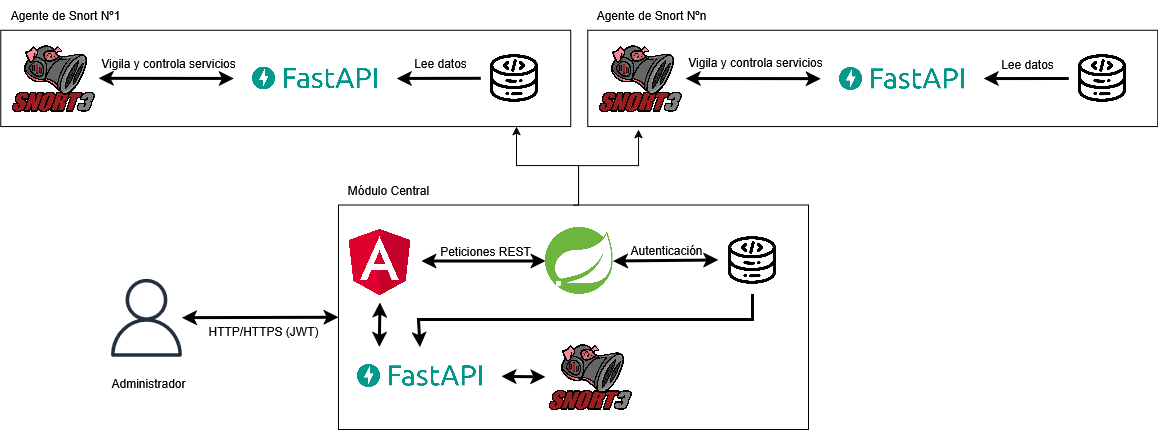
\includegraphics[width=0.8\textwidth]{documento/6.png}
	\caption{Esquema de la arquitectura distribuida de R-Snort.}
	\label{fig:arquitectura}
\end{figure}

El diseño plug-and-play de R-Snort aunque orientado para administradores de sistemas y seguridad, se ha creado para que cualquiera con conocimientos mínimos de Linux sea capaz de instalarlo: agregar un nuevo sensor es tan simple como instalar un agente en el nuevo equipo e informarlo al sistema central, sin configuraciones manuales complejas. Esta aproximación aporta sencillez en entornos de ciberseguridad distribuida, ya que ofrece visibilidad unificada de múltiples sensores de intrusión. Cada agente opera de manera autónoma en su segmento de red, pero todos son gestionados centralmente, lo que aumenta la cobertura de detección y la resiliencia (si un sensor falla o es comprometido, los demás continúan operativos y reportando al panel central).

\subsection{Diseño de la interfaz de usuario}

\subsubsection{Frontend web (Angular SPA)}

El sistema cuenta con una interfaz web de usuario desarrollada en Angular, construida como una \emph{Single Page Application} (\textbf{SPA}) independiente que se comunica con el backend mediante peticiones HTTP a la API REST central. Esta aplicación frontend, desplegada en el servidor central, ofrece una experiencia interactiva y dinámica, con un diseño visual enfocado en el dominio de la ciberseguridad. La usabilidad se ha cuidado para que la información compleja de las alertas y métricas se presente de forma accesible y atractiva incluso para operadores no especializados.\newline

La interfaz de usuario se estructura en varios módulos o pantallas principales, accesibles desde una barra de navegación superior:\newline

\begin{itemize}
	\item \textbf{Inicio de sesión:} es la pantalla inicial de la aplicación, donde el usuario introduce sus credenciales (\emph{correo electrónico} y \emph{contraseña}) para acceder. Tras hacer clic en "Acceder", el backend valida las credenciales y, de ser correctas, emite un token de autenticación JWT. La apariencia de esta vista es sencilla y centrada (formulario sobre fondo oscuro, como se aprecia en la Figura 2.4.2), siguiendo las pautas de diseño minimalista.
	
	\item \textbf{Selector de agente:} una vez autenticado, el usuario puede seleccionar cuál de los agentes disponibles desea monitorizar. En la barra superior de la SPA se muestra un menú desplegable que lista los agentes registrados (identificados por nombre o dirección IP, e.g. "Central (192.168.1.169)"). Al elegir un agente, el frontend carga los datos correspondientes a ese sensor en las vistas de alertas, reglas y estado. Este mecanismo permite controlar múltiples sensores desde la misma interfaz de forma conveniente.
	
	\item \textbf{Vista de alertas:} es el panel principal de monitorización, donde se presentan las detecciones de intrusiones reportadas por Snort en el agente seleccionado. Incluye indicadores numéricos de alertas por nivel de severidad (ej. cantidad de alertas altas, medias, bajas) y una tabla que enumera las últimas alertas detalladas con sus campos clave (hora, descripción de la alerta, IP de origen, IP de destino, puerto implicado, clasificación de la alerta y nivel de severidad). Esta vista permite al analista ver rápidamente qué incidentes se han detectado y su naturaleza. Además, proporciona botones para exportar los datos de alertas en formato CSV: por ejemplo, "Descargar alertas de este agente" genera un archivo con todas las alertas actuales del sensor activo, mientras que "Descargar todas las alertas" consolida las alertas de todos los agentes en un solo fichero (facilitando un análisis global). En la Figura 2.4.3 se ilustra un ejemplo de esta pantalla, mostrando el \emph{Panel de Alertas} con los contadores de severidad y la tabla de alertas recientes.
	
	\item \textbf{Vista de reglas:} sección de la aplicación dedicada a la gestión de reglas personalizadas de Snort en el agente seleccionado. Permite al usuario con rol adecuado agregar nuevas reglas de detección escribiendo la definición en formato Snort en un campo de texto y pulsando "Agregar regla". Una vez enviada, la regla se almacena a través del backend en el agente correspondiente (el \texttt{snort-agent} la añade a la configuración de Snort y recarga el motor de detección para que la nueva regla entre en vigor). Asimismo, en esta vista se listan todas las reglas personalizadas previamente añadidas al sensor, mostrando por cada una su \texttt{SID} (identificador único), el mensaje descriptivo (\texttt{MSG}) y la sintaxis completa de la regla. Junto a cada regla se presenta una opción (icono de papelera) para eliminarla si es necesario, lo cual provoca que el agente la remueva de Snort (actualizando la configuración). La Figura 2.4.4 muestra la interfaz de esta vista de reglas, donde se observan el formulario de nueva regla y la lista de reglas existentes con sus detalles.
	
	\item \textbf{Vista de estado del sistema:} pantalla orientada a visualizar las métricas operativas del agente y el estado del servicio Snort. Contiene gráficas en tiempo real de los datos del sistema recabados (por ejemplo, un gráfico de línea de la temperatura de CPU del sensor, y otro del porcentaje de uso de CPU y de disco a lo largo del tiempo). Estos gráficos ofrecen al usuario una idea del rendimiento y condiciones del hardware donde corre Snort, ayudando a detectar posibles sobrecargas o problemas (p.ej., temperatura anómala). Además, esta vista muestra el estado actual de Snort en ese agente: indica si el proceso IDS está \emph{Activo} y la marca de tiempo de la última alerta registrada. Si el usuario cuenta con permisos de administrador, desde aquí puede reiniciar remotamente el servicio Snort en el agente seleccionado mediante un botón dedicado ("Reiniciar Snort"). También se listan en esta página los \emph{logs} archivados (ficheros históricos de alertas comprimidos tras la rotación de logs); el usuario puede descargarlos para un análisis forense si es necesario. En la Figura 2.4.5 se aprecia esta sección, incluyendo un ejemplo de gráfico de temperatura CPU y los indicadores de estado del agente.
	
	\item \textbf{Overview e integración con Grafana:} la página inicial del panel (denominada \emph{Overview}) ofrece un resumen gráfico consolidado de la información de seguridad. Esta vista integra paneles de visualización tipo \emph{dashboard} para representar las alertas y eventos de forma gráfica y amigable, aprovechando herramientas como Grafana para las métricas de serie temporal. Por ejemplo, se muestran diagramas de dona con la distribución de alertas por severidad o por tipo, gráficas de líneas con el volumen de eventos en el tiempo y otros gráficos interactivos que ayudan a identificar patrones de ataque de un vistazo. La integración con Grafana permite reutilizar su potente motor de gráficos para presentar datos de los agentes dentro de la propia interfaz de R-Snort, manteniendo la consistencia del estilo visual oscuro y profesional.
\end{itemize}

\subsubsection{Mecanismo de autenticación y control de acceso}

El frontend utiliza autenticación basada en \textbf{JWT}: tras iniciar sesión, el token JWT proporcionado por el backend se adjunta a cada petición subsiguiente, garantizando que solo usuarios autenticados (y con rol adecuado) accedan a los recursos. Asimismo, la aplicación cliente refleja en todo momento el estado de los agentes: se realiza una comprobación periódica de disponibilidad de cada sensor, ya sea mediante \emph{ping} de red o invocando el endpoint \texttt{/status} de su API. Si un agente no responde (caído o desconectado), el panel lo indicará claramente (por ejemplo, marcándolo como inactivo o mostrando una alerta visual), permitiendo al usuario identificar problemas de conectividad o fallos en los sensores de forma proactiva.

\subsection{Esquema de la base de datos}

Para almacenar la información de alertas de intrusión, métricas del sistema y credenciales de usuarios, R-Snort emplea una base de datos relacional MariaDB. El esquema se ha mantenido sencillo, definiendo tres tablas principales: \texttt{alerts}, \texttt{system\_metrics} y \texttt{users}. A continuación se presenta la estructura SQL de cada tabla junto con una breve descripción de su contenido y función.\newline

La tabla \texttt{alerts} almacena cada evento de alerta generado por Snort en los agentes. Cada fila corresponde a una alerta detectada e incluye los detalles más relevantes: fecha y hora del evento, dirección IP de origen, dirección IP de destino, puerto implicado, descripción o mensaje de la alerta, clasificación asignada por Snort (p.ej. tipo de ataque o categoría) y nivel de severidad (prioridad). Esta tabla es alimentada en tiempo real por el componente \texttt{ingest\_service.py} de cada agente, que inserta un nuevo registro cada vez que Snort produce una alerta. De este modo, \texttt{alerts} actúa como el registro histórico de incidentes detectados por cada sensor.\newline

\begin{figure}[H]
	\centering
	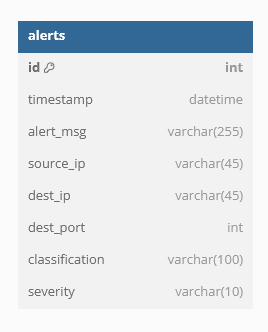
\includegraphics[width=0.4\textwidth]{documento/7.png}
	\caption{Tabla alertas.}
	\label{fig:alertas-bd}
\end{figure}

Por su parte, la tabla \texttt{system\_metrics} guarda las mediciones periódicas del estado de cada equipo monitorizado. Cada registro representa una muestra tomada por \texttt{metrics\_timer.py} e incluye la marca temporal del muestreo junto con los valores de parámetros como porcentaje de CPU en uso, porcentaje de espacio de disco utilizado y temperatura de la CPU en grados Celsius, entre otros posibles indicadores del rendimiento del sistema. La frecuencia de inserción en esta tabla depende de la configuración del agente (por ejemplo, cada minuto o cada pocos minutos se añade un nuevo registro). Gracias a estos datos, el administrador puede consultar históricos de rendimiento y detectar condiciones anómalas (como un sobrecalentamiento sostenido o falta de recursos) a través de las gráficas en la interfaz.\newline

\begin{figure}[H]
	\centering
	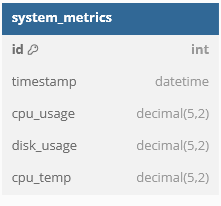
\includegraphics[width=0.4\textwidth]{documento/8.png}
	\caption{Tabla métricas.}
	\label{fig:metricas-bd}
\end{figure}

Finalmente, la tabla \texttt{users} contiene las cuentas de usuario autorizadas para ingresar al panel de control de R-Snort. Por motivos de seguridad, en esta tabla se almacenan las credenciales de forma cifrada (la contraseña se guarda típicamente con un hash irreversible, nunca en texto plano). Los campos principales incluyen el correo electrónico del usuario (que funciona como nombre de usuario para el inicio de sesión), la contraseña hasheada. Esta información es gestionada por el backend Spring Boot: durante el proceso de autenticación se verifica la combinación de email y contraseña contra los registros de \texttt{users} y, si coincide, se genera el JWT correspondiente.\newline

\begin{figure}[H]
	\centering
	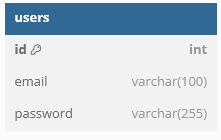
\includegraphics[width=0.4\textwidth]{documento/9.png}
	\caption{Tabla usuario.}
	\label{fig:usuario-bd}
\end{figure}

Con estas tres tablas, el sistema almacena de forma organizada tanto los eventos de seguridad recopilados por los sensores (\texttt{alerts}), como los datos de rendimiento de los mismos (\texttt{system\_metrics}) y la información de quienes administran o supervisan la plataforma (\texttt{users}). El diseño relacional simplificado facilita las consultas necesarias: el backend puede obtener rápidamente las alertas filtrando por fecha, severidad u otros campos; extraer series de métricas para graficar en el dashboard; y verificar credenciales de inicio de sesión con consultas eficientes. Además, al mantener la base de datos en MariaDB (un sistema ampliamente soportado), se garantiza confiabilidad, rendimiento suficiente para los volúmenes de datos manejados, y la posibilidad de escalar o realizar copias de seguridad de la información de manera estándar.

\begin{figure}[H]
	\centering
	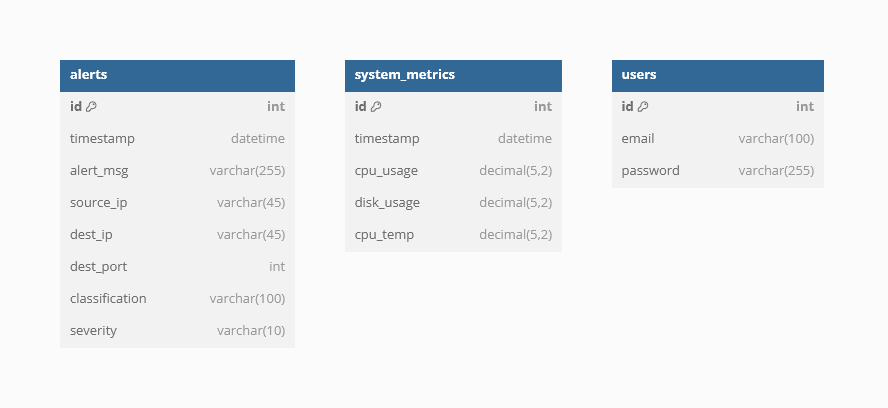
\includegraphics[width=0.8\textwidth]{documento/10.png}
	\caption{Tablas base de datos.}
	\label{fig:esquema-bd}
\end{figure}

\newpage

\section{Implementación y configuración del sistema}

Partiendo de una instalación estándar de Snort 3, se llevó a cabo una serie de configuraciones y desarrollos adicionales para convertirlo en un agente IDS autónomo, monitorizable y funcional (denominado snort-agent). En esta sección se detallan estos pasos, desde la habilitación de un registro estructurado de alertas en formato JSON hasta la integración de un panel de control en Grafana respaldado por MariaDB. El resultado es un agente capaz de generar alertas procesables, registrar métricas operativas y exponer su estado a sistemas externos, sentando las bases para su posterior automatización.

\subsection{Snort 3: configuración de salida de alertas en JSON}

El primer paso fue modificar la configuración por defecto de Snort 3 para que las alertas se registraran en formato JSON, lo que facilita su posterior tratamiento automático. Snort 3 tiene un \textit{plugin} de \textit{logging} llamado \texttt{alert\_json} que permite volcar cada alerta generada como una entrada JSON estructurada. Para habilitarlo, se editó el fichero de configuración principal (por defecto, \texttt{snort.lua}) en la sección de outputs, añadiendo un bloque de configuración específico para \texttt{alert\_json}. En el Código \ref{lst:snort-json} se muestra un extracto resumido de esta configuración:

\begin{lstlisting}[language=bash, caption={Configuración de Snort~3 para salida de alertas en JSON}, label={lst:snort-json}]
	alert_json =
	{
		file = true, -- habilita salida a archivo (no solo consola)
		limit = 50, -- tamaño (MB) tras el cual se rota el archivo
		fields = 'timestamp src_addr src_port dst_addr dst_port proto msg sid priority classtype ...'
	}
\end{lstlisting}

En esta configuración, se indica a Snort que vuelque las alertas en un archivo (en lugar de la salida estándar de consola) y se establece un límite de tamaño (\texttt{limit}) para que, al alcanzar 50MB, Snort rote automáticamente al siguiente archivo de alerta (evitando que un único fichero crezca indefinidamente). Además, mediante la opción \texttt{fields}, se especifica el conjunto de campos de cada alerta que serán incluidos en el JSON. En nuestro caso se optó por incluir todos los campos relevantes: marca de tiempo, direcciones IP origen y destino, puertos, protocolo, mensaje/descripción de la alerta, identificadores de regla (sid/rev), clasificación (\textit{classtype}) y severidad (\textit{priority}), entre otros. Esta salida facilita la ingesta automatica. Cabe mencionar que Snort 3 añade por defecto un campo numérico de tiempo (\texttt{seconds}) al inicio del JSON para asegurar un ordenado procesado temporal. Tras habilitar \texttt{alert\_json}, Snort deja de imprimir alertas por pantalla y las escribe en el archivo designado (\texttt{/var/log/snort/alert\_json.txt}), listo para ser procesado por otros componentes del sistema.\newline

Finalmente, para ejecutar Snort de forma persistente como agente en segundo plano, se configuró un servicio del sistema (systemd). Se creó un fichero de unidad \path{/etc/systemd/system/snort.service} que inicia Snort con unos determinados parámetros: la interfaz de red a monitorizar, el fichero de configuración \texttt{snort.lua} y el directorio de logs. De este modo, el IDS se inicia automáticamente al encender el sistema y permanece activo como \textit{daemon}, escribiendo sus alertas en formato JSON en el archivo configurado.

\subsubsection{Servicio de ingesta de alertas en base de datos}

Con las alertas de Snort ya estructuradas en JSON, se implementó un servicio auxiliar de \textbf{ingesta} cuyo cometido es leer continuamente el archivo de alertas JSON y volcar la información a una base de datos MariaDB. Este servicio actúa como puente entre Snort y el sistema de monitorización, extrayendo los datos de cada alerta y almacenándolos en las tablas correspondientes donde pueden ser consultados fácilmente por otras herramientas (p.~ej., Grafana).\newline

Para su implementación se desarrolló un proceso demonizado (en este caso, un script en Python) que se lanza junto con Snort. Dicho proceso abre el archivo de alertas (\path{alert\_json.txt}) en modo lectura continua y espera nuevos eventos. Cada vez que Snort escribe una nueva línea JSON, el servicio de ingesta la detecta, la parsea (utilizando una biblioteca JSON estándar) y extrae los campos de interés. A continuación, construye una sentencia \texttt{INSERT} para añadir la alerta a la base de datos. En la tabla \texttt{alertas} de MariaDB, cada registro almacena los campos principales de una alerta: marca de tiempo, IP origen, IP destino, puertos, protocolo, severidad, clasificación y mensaje de la alerta, entre otros. De este modo, cada alerta queda persistida. El proceso se asegura de manejar correctamente el flujo continuo de alertas (por ejemplo, manteniendo el fichero abierto y leyendo línea a línea conforme crece, similar al comando \texttt{tail -f}). Asimismo, ante una rotación del archivo de log (discutida más adelante), el servicio de ingesta está preparado para cerrar y reabrir el nuevo fichero sin interrumpir la captura de eventos.\newline

Este enfoque aporta varias ventajas. Primero, las consultas SQL permiten filtrar y agregar alertas de forma flexible (por ejemplo, obtener conteos por tipo de alerta o por IP origen). Segundo, MariaDB facilita la gestión del histórico de alertas, a la vez que permite acceso concurrente desde múltiples aplicaciones (por ejemplo, la API del agente o el dashboard). Por último, se añadió a cada inserción un identificador del agente (un ID único para cada despliegue de R-Snort) para posibilitar entornos con múltiples sensores: de esta forma, una instancia centralizada de la base de datos puede distinguir el origen de las alertas y consolidar la información de varios agentes.

\begin{lstlisting}[language=Python, caption={Esquema simplificado del servicio de ingesta de alertas}, label={lst:ingest}]
	conn = mysql.connector.connect(user="snort", password="...", database="snortDB") #Implementación real con variables de entorno
	cursor = conn.cursor()
	f = open("/var/log/snort/alert_json.txt", "r")
	f.seek(0, 2) # Ir al final del archivo
	while True:
	line = f.readline()
	if not line:
	time.sleep(1); continue # Esperar datos nuevos
	alert = json.loads(line)
	cursor.execute(
	"INSERT INTO alertas(timestamp, src_ip, dst_ip, proto, puerto, severidad, clase, mensaje, agente_id) "
	"VALUES (%s,%s,%s,%s,%s,%s,%s,%s,%s)",
	(alert["timestamp"], alert["src_addr"], alert["dst_addr"], alert["proto"],
	alert["dst_port"], alert["priority"], alert["class"], alert["msg"], AGENTE_ID))
	conn.commit()
\end{lstlisting}

El Código \ref{lst:ingest} muestra la lógica descrita: el servicio se conecta a MariaDB, abre el fichero de alertas y entra en un bucle infinito leyendo nuevas líneas JSON según aparecen. Cada alerta se convierte de JSON a estructuras de datos (\texttt{alert}) y se inserta en la tabla \texttt{alertas} mediante una consulta SQL parametrizada. Nótese que en una implementación real se incluyen consideraciones adicionales (manejo de errores de conexión, reconexión en caso de reinicio de la base de datos, etc.), pero a grandes rasgos este mecanismo garantiza que todas las alertas generadas por Snort queden almacenadas en la base de datos en tiempo real.

\begin{figure}[H]
	\centering
	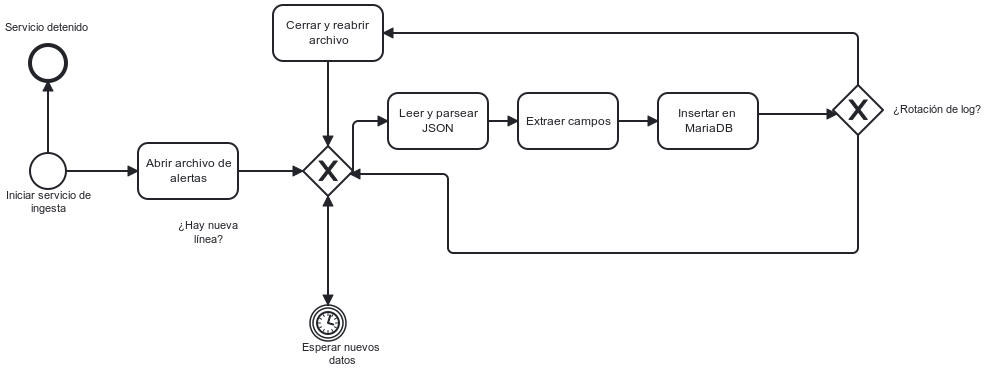
\includegraphics[width=1\textwidth]{documento/23.png}
	\caption{BPMN del servicio de ingesta de alertas.}
	\label{fig:bpmn-servicio-ingesta}
\end{figure}

\subsubsection{Servicio de métricas y monitorización del agente}

Además de las alertas, el agente R-Snort recopila y expone métricas operativas que permiten monitorizar su estado y rendimiento. Para ello se desplegó un segundo servicio auxiliar encargado de recolectar periódicamente datos como el uso de CPU y memoria del proceso Snort, el estado de sus interfaces de captura, etc. Algunas de estas métricas se obtienen directamente de la base de datos de alertas (por ejemplo, un conteo de alertas por severidad en la última hora), mientras que otras provienen del propio sistema operativo (por ejemplo, consultando /proc para recursos utilizados por Snort).\newline

Este servicio de métricas corre en segundo plano y vuelca los datos recopilados también en la base de datos MariaDB, en tablas diseñadas para métricas. Por ejemplo, se define una tabla \texttt{metricas} donde cada registro puede contener el timestamp, el nombre de la métrica y el valor observado en ese momento (p.ej., \textit{cpu\_usage} = 30\%). De esta forma, se va construyendo un historial temporal no solo de eventos de seguridad (alertas) sino también de indicadores de rendimiento del sensor.\newline

Al igual que el servicio de ingesta, el servicio de métricas está pensado para ejecutarse automáticamente al iniciar el agente. Se ha optado por integrarlo en el propio agente para simplificar la coordinación. Este componente rellena las tablas de métricas en MariaDB y también expone la información importante a través de la API REST del agente (por ejemplo, un endpoint \verb|GET /metrics| devuelve las últimas métricas recopiladas, facilitando integraciones externas).

\begin{figure}[H]
	\centering
	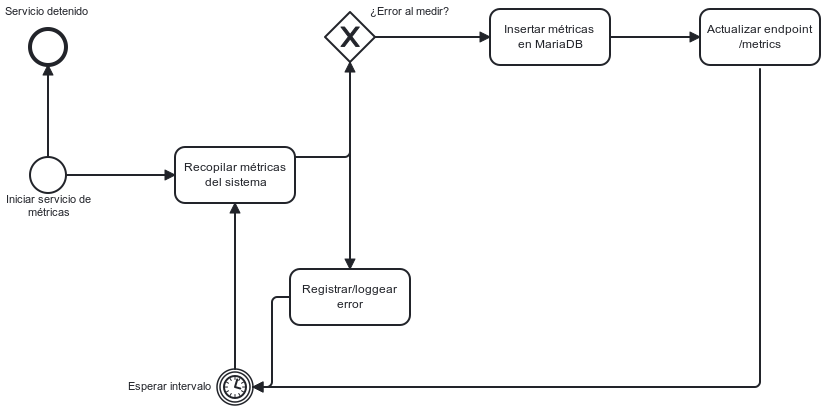
\includegraphics[width=1\textwidth]{documento/24.png}
	\caption{BPMN del servicio de ingesta de métricas.}
	\label{fig:bpmn-servicio-metricas}
\end{figure}

\subsubsection{Rotación y archivado de logs de Snort}

Dado el carácter continuo de la monitorización, es de vital importancia gestionar los ficheros de registro que Snort genera, evitando tanto la pérdida de información como el consumo ilimitado de espacio en disco. Para ello se implementó una estrategia combinada de rotación y archivado de logs.\newline

Por un lado, como ya se indicó, Snort 3 rota internamente el archivo de alertas JSON cuando este alcanza un tamaño predefinido (\texttt{limit} en la configuración). En el despliegue, se eligió un límite (p.ej., 50MB) de modo que, al superarse, Snort cierre \texttt{alert\_json.txt} y comience un nuevo archivo (generalmente nombrado con un sufijo temporal, por ejemplo \texttt{alert\_json.txt.1684500000} usando la época Unix para garantizar un nombre único). Esto asegura que el archivo activo de alertas se mantenga de un tamaño manejable para el servicio de ingesta y que las alertas antiguas queden preservadas en ficheros aparte.\newline

Por otro lado, para gestionar esos ficheros históricos y evitar la acumulación indefinida, se configuró la herramienta \textbf{logrotate} en el sistema. Se añadió una regla específica para los logs de Snort en \texttt{/etc/logrotate.d/}, de forma que diariamente (o bajo ciertas condiciones de tamaño) se compriman y archiven los archivos de alerta rotados. La configuración de \textit{logrotate} establece, por ejemplo, mantener solo los N archivos más recientes (p.ej., los últimos 7 días de alertas), comprimir automáticamente los logs rotados (formato \texttt{.gz}) y eliminar aquellos que excedan el período de retención. A continuación se muestra un extracto de dicha configuración:

\newpage

\begin{lstlisting}[language=bash, caption={Regla de logrotate para los logs de Snort}, label={lst:logrotate}]
	/var/log/snort/alert_json.txt* {
		daily
		rotate 7
		compress
		missingok
		notifempty
		postrotate
		systemctl reload snort3.service > /dev/null 2>&1 || true
		endscript
	}
\end{lstlisting}

En el ejemplo del Listado~\ref{lst:logrotate}, \texttt{logrotate} rotará cualquier fichero que comience con \path{alert\_json.txt} (incluyendo los generados por Snort al alcanzar el límite de tamaño) de forma diaria, conservando un máximo de 7 días de logs y comprimiendo los antiguos. La sección \texttt{postrotate} envía una señal de recarga a Snort tras la rotación, para garantizar que Snort vuelva a abrir correctamente el nuevo fichero de log (esto es relevante sobre todo si por alguna razón se rotase el fichero activo antes de que Snort lo haga por su cuenta). Gracias a este mecanismo combinado, el sistema mantiene un archivo \textit{activo} de alertas para ingestión en tiempo real, a la vez que almacena de forma segura los archivos históricos de alertas (ya comprimidos) en caso de que se requiera algún análisis forense o consulta retroactiva de eventos.

\begin{figure}[H]
	\centering
	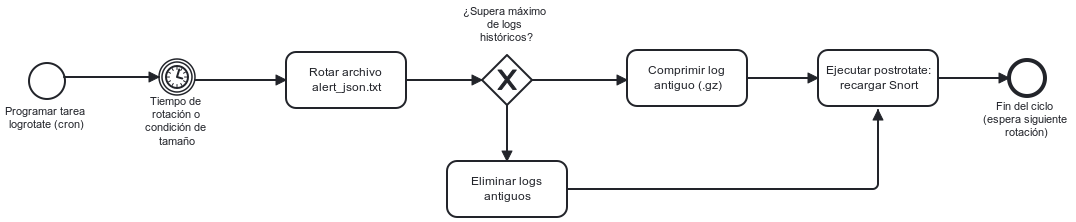
\includegraphics[width=1\textwidth]{documento/25.png}
	\caption{BPMN del servicio de logrotate y archivado.}
	\label{fig:bpmn-logrotate}
\end{figure}

\subsubsection{Integración de Grafana con base de datos MariaDB}

Una vez que las alertas y métricas de Snort se encuentran almacenadas en MariaDB, se procedió a integrar una instancia de \textbf{Grafana} para visualizar dicha información de manera dinámica e interactiva. Grafana es una plataforma de visualización de series temporales y datos operativos que, mediante paneles (dashboards) personalizables, permite monitorear tanto las alertas de seguridad generadas por Snort como el estado del propio agente.\newline

En primer lugar, se configuró Grafana para que utilizara a MariaDB como fuente de datos. Grafana soporta MySQL/MariaDB mediante un conector nativo, por lo que se creó un \textit{Data Source} de tipo MySQL apuntando al servidor MariaDB donde residían las tablas de alertas y métricas. Se le proporcionaron las credenciales de solo-lectura adecuadas. A continuación, se diseñó el dashboard de Grafana. Para acelerar este desarrollo, se partió de una plantilla pública existente para Snort (originalmente creada para stacks ELK/InfluxDB) y se adaptó a la solución basada en MariaDB \cite{grafana-dashboard}. Concretamente, se tomó como referencia el dashboard \emph{Snort IDS/IPS} (ID 11191 en Grafana), reaprovechando su disposición y elementos visuales (gráficas de líneas, tablas, paneles de métricas clave, mapas, etc.), pero modificando las consultas de datos para ajustarlas al esquema SQL de nuestro sistema y a las métricas disponibles.\newline

En la adaptación, cada panel del dashboard original fue traducido a una consulta SQL equivalente. Por ejemplo, donde el template original empleaba una consulta en InfluxQL (InfluxDB) para contar eventos por severidad o tipo de ataque, ahora se utiliza una consulta SQL sobre la tabla \texttt{alertas} agrupando por el campo de severidad o clasificación. Del mismo modo, los paneles que muestran series temporales (ej.~número de alertas en el tiempo, tráfico por protocolo) se implementaron con consultas SQL que aprovechan las funciones de tiempo de MariaDB (p.~ej., agrupando por minuto u hora usando \texttt{DATE\_FORMAT} o funciones UNIX\_TIMESTAMP). A continuación se presenta una consulta simplificada empleada en el panel de “top protocolos” del dashboard adaptado:

\begin{lstlisting}[language=SQL, caption={Consulta SQL (simplificada) para panel de protocolos en Grafana}, label={lst:sql-proto}]
	SELECT proto AS protocolo, COUNT(*) AS total_alertas
	FROM alertas
	WHERE timestamp >= DATE_SUB(NOW(), INTERVAL 24 HOUR)
	GROUP BY proto
	ORDER BY total_alertas DESC;
\end{lstlisting}

Esta consulta (Código \ref{lst:sql-proto}) devuelve el número de alertas detectadas en un intervalo de tiempo de red observado, ordenando de mayor a menor frecuencia. Consultas similares se prepararon para otros paneles: conteo de alertas por nivel de severidad (mapeando el campo numérico \texttt{priority} de Snort a etiquetas descriptivas “Alta”, “Media”, “Baja”), listados de las “Top N” reglas disparadas, direcciones IP de origen más frecuentes en las alertas, y gráficos de series temporales mostrando la evolución de alertas en el tiempo. También se incorporó un panel tipo tabla para mostrar el detalle de las últimas alertas registradas (hora, descripción, IP de origen y destino, puerto, clasificación y severidad), obteniendo directamente los registros más recientes de la tabla \texttt{alertas}.

\begin{figure}[htb]
	\centering
	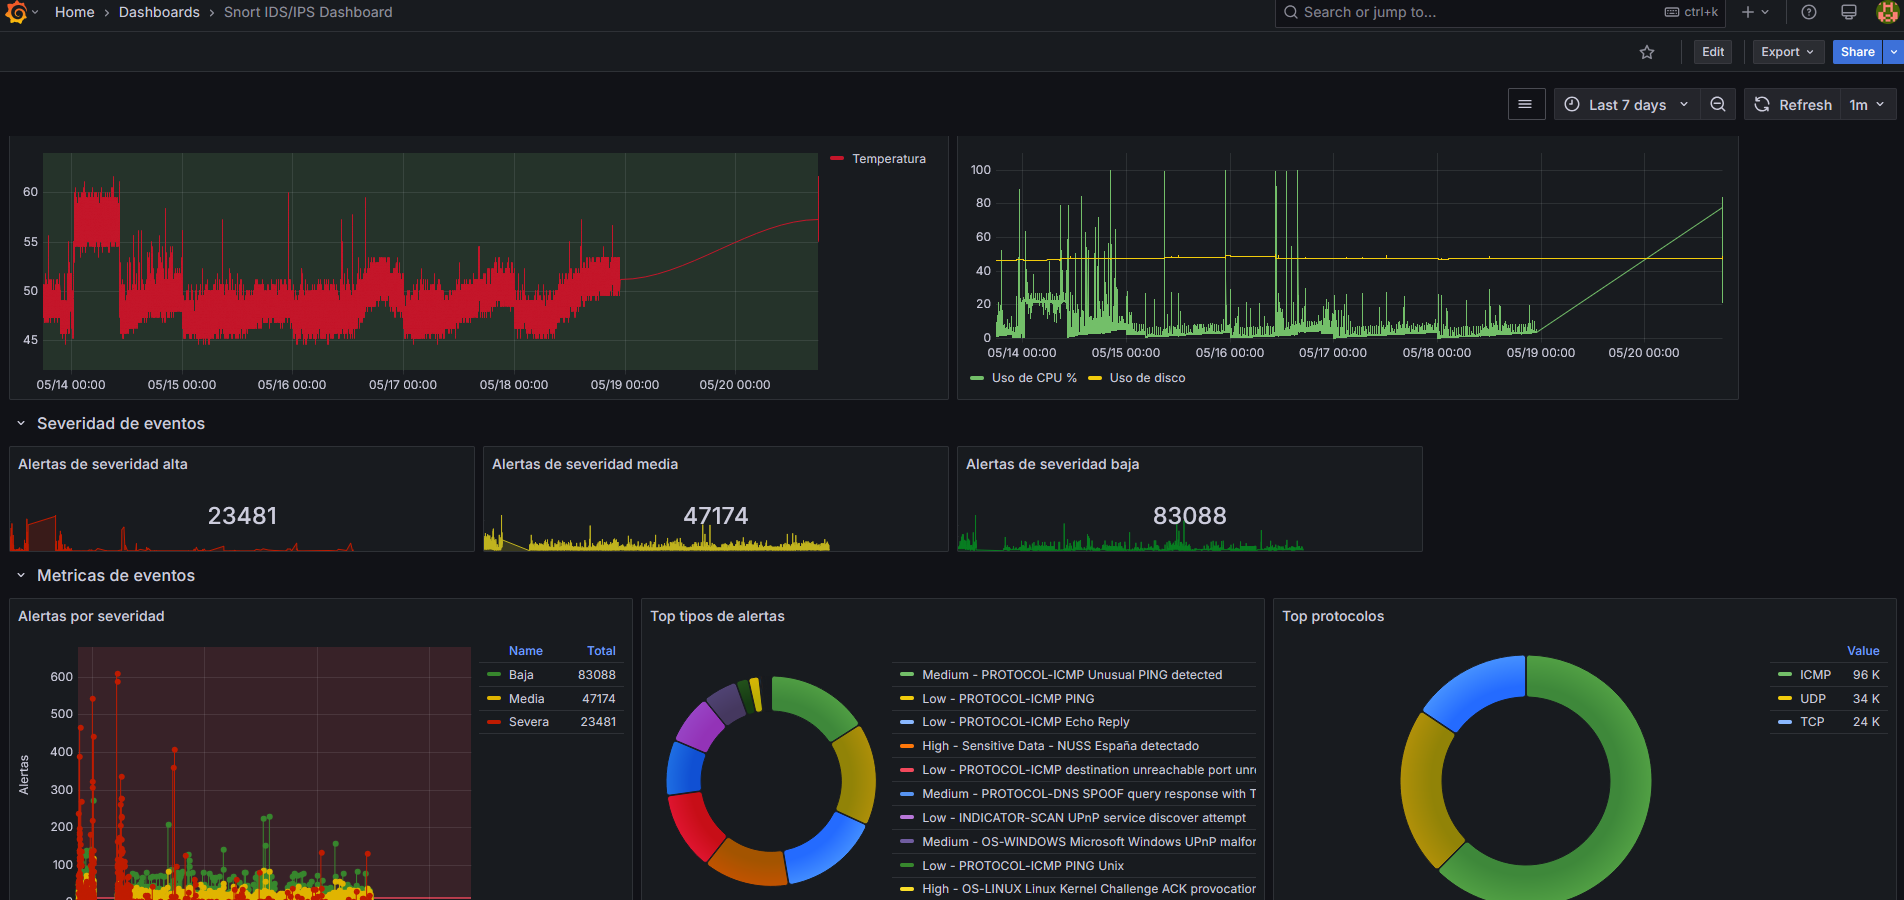
\includegraphics[width=0.95\textwidth]{documento/grafana1.png}
	\caption{Dashboard de Grafana adaptado para R-Snort.}
	\label{fig:grafana-dashboard}
\end{figure}

La Figura~\ref{fig:grafana-dashboard} muestra una captura del dashboard resultante. Este panel de control ofrece una vista unificada del estado de seguridad monitorizado por el agente: en la parte superior, métricas agregadas como el número de alertas recientes categorizadas por severidad; en el centro, gráficas de pastel destacando los principales tipos de alerta detectados y los protocolos de red involucrados; a la derecha, los IP de origen más comunes en las alertas (potenciales fuentes maliciosas); y en la parte inferior, una tabla actualizada con las últimas alertas generadas, permitiendo al analista ver detalles puntuales de cada evento de seguridad.\newline

Para lograr que este dashboard esté disponible inmediatamente tras desplegar un agente R-Snort, se automatizó su provisión. Se preparó el JSON de la plantilla adaptada y, durante el proceso de instalación del agente, un script de configuración importa dicho dashboard en Grafana de forma programática (utilizando la API HTTP de Grafana o su mecanismo de \textit{provisioning}). De esta manera, el usuario no necesita configurar manualmente el panel: una vez que Grafana arranca apuntando a la base de datos de Snort, el dashboard personalizado aparece pre-cargado y listo para su uso. Esta automatización reduce posibles errores de configuración y asegura la consistencia del entorno de monitorización en todos los despliegues del sistema.\newline

En resumen, mediante la integración con Grafana se concreta la faceta “monitorizable” de R-Snort: el administrador de seguridad dispone de una interfaz gráfica intuitiva desde la cual puede supervisar en tiempo real la actividad del IDS y la salud del agente. La combinación de alertas almacenadas en MariaDB con visualizaciones de Grafana adaptadas a dichas alertas proporciona una solución ligera pero efectiva, que cubre las necesidades de un SIEM básico: detección (Snort), recolección/almacenamiento (servicio de ingesta + base de datos) y presentación de información (Grafana) en un solo sistema cohesionado.

\begin{figure}[htb]
	\centering
	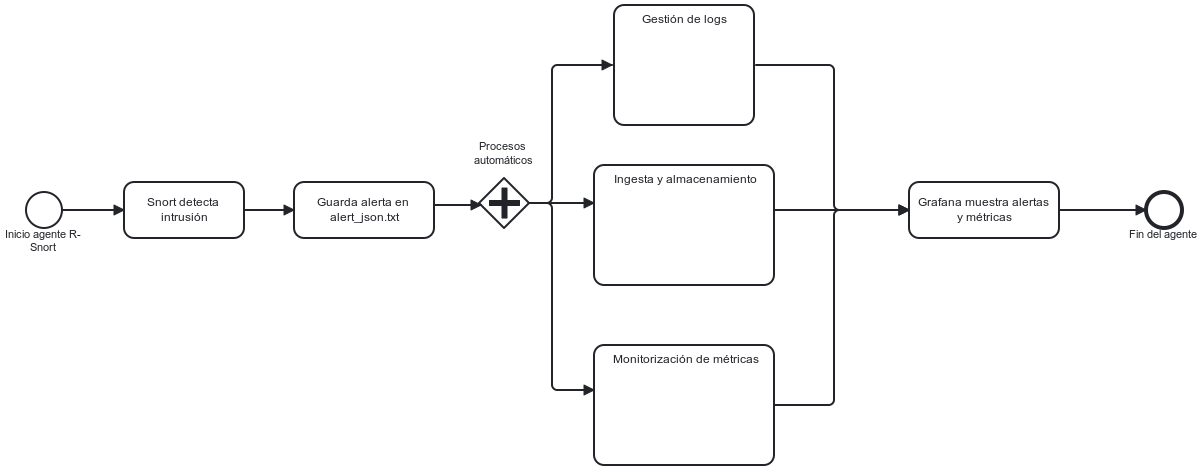
\includegraphics[width=1\textwidth]{documento/26.png}
	\caption{Diagrama de funcionamiento del agente.}
	\label{fig:agent-bpmn}
\end{figure}

\subsection{Implementación del backend}

El sistema R-Snort cuenta con una arquitectura de backend dividida en dos partes principales: un backend de agentes, implementado con FastAPI (Python) y ejecutado en cada nodo sensor; y un backend central, desarrollado en Spring Boot (Java), que coordina la información de todos los agentes y provee servicios a la interfaz web. A continuación se detallan ambos componentes en términos de endpoints, arquitectura y mecanismos de seguridad

\subsubsection{Backend de los agentes (FastAPI)}

Cada agente R-Snort ejecuta un servicio web ligero construido con FastAPI, el cual expone múltiples endpoints REST para monitorear y controlar remotamente el sensor. Estos endpoints permiten consultar el estado de Snort, obtener las alertas detectadas, extraer métricas del sistema, gestionar las reglas personalizadas de detección y manejar archivos de registro, entre otras acciones.


\begin{figure}[htb]
	\centering
	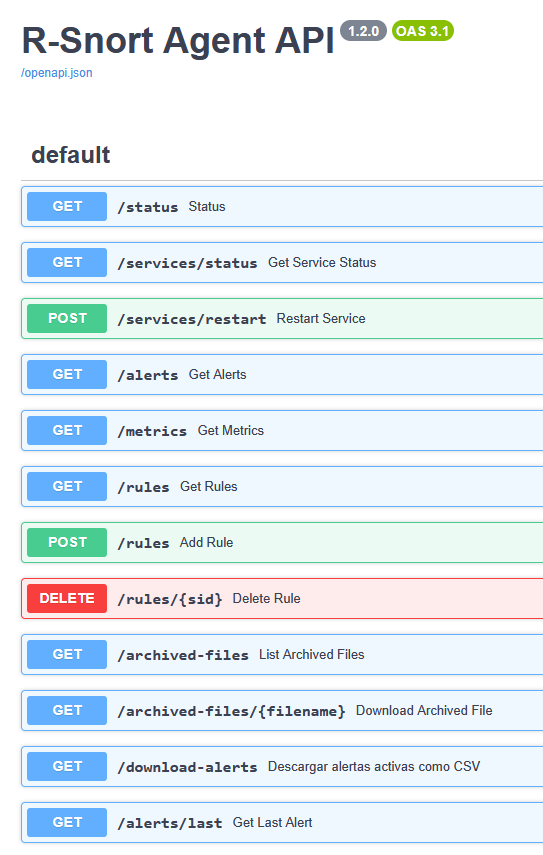
\includegraphics[width=0.5\textwidth]{documento/13.png}
	\caption{Documentación Swagger de la API de un agente R-Snort.}
	\label{fig:fastapi}
\end{figure}

\begin{table}[H]
	\centering
	\resizebox{\textwidth}{!}{%
		\begin{tabular}{|c|l|p{11cm}|}
			\hline
			\textbf{Método} & \textbf{Endpoint} & \textbf{Funcionalidad} \\
			\hline
			GET & \texttt{/status} & Obtener un estado básico del agente (sirve como \textit{ping} de salud). \\
			\hline
			GET & \texttt{/services/status} & Consultar el estado de los servicios internos del agente (por ejemplo, si Snort y otros procesos están activos). \\
			\hline
			\textbf{POST} & \texttt{/services/restart} & Reiniciar el servicio de detección en el agente (p.ej., reinicia el proceso Snort u otro servicio especificado). \\
			\hline
			GET & \texttt{/alerts} & Listar las alertas recientes o activas detectadas por Snort en ese agente. \\
			\hline
			GET & \texttt{/metrics} & Obtener métricas del sistema local (uso de CPU, memoria, temperatura, etc.) del agente. \\
			\hline
			GET & \texttt{/rules} & Listar las reglas de Snort en el agente, incluyendo reglas personalizadas añadidas. \\
			\hline
			\textbf{POST} & \texttt{/rules} & Añadir una nueva regla de Snort personalizada en el agente. El cuerpo de la petición incluye la regla en formato Snort. \\
			\hline
			\textbf{DELETE} & \texttt{/rules/\{sid\}} & Eliminar una regla personalizada identificada por su SID del conjunto de reglas del agente. \\
			\hline
			GET & \texttt{/archived-files} & Listar archivos de log archivados en el agente (logs históricos de alertas, comprimidos o rotados). \\
			\hline
			GET & \texttt{/archived-files/\{filename\}} & Descargar un archivo de log archivado específico desde el agente. \\
			\hline
			GET & \texttt{/download-alerts} & Descargar todas las alertas activas del agente en formato CSV. \\
			\hline
			GET & \texttt{/alerts/last} & Obtener la información de la última alerta detectada por el agente. \\
			\hline
		\end{tabular}
	} % Fin de \resizebox
	\caption{Resumen de los endpoints expuestos por el backend del agente R-Snort.}
	\label{tab:endpoints-agente}
\end{table}


En términos de implementación, cada endpoint del agente está manejado por una función Python utilizando FastAPI. Por ejemplo, un fragmento simplificado para eliminar una regla podría ser:

\begin{lstlisting}[language=Python, caption={Fragmento del código que maneja cada endpoint}, label={lst:ejemplo-endpoint}]
@app.delete("/rules/{sid}")
def delete_rule(sid: int):
# Eliminar la regla con el SID dado del archivo de reglas de Snort
	if remove_rule_from_file(sid):
		return {"detail": "Regla eliminada"}
	raise HTTPException(status_code=404, detail="Regla no encontrada")
\end{lstlisting}

Mediante estos endpoints, el backend de un agente permite al servidor central y a la interfaz web consultar y modificar el estado de ese sensor. La comunicación se realiza a través de HTTP: el backend central invoca las rutas del agente según sea necesario. Por ejemplo, si el usuario solicita ver las alertas de un agente en la interfaz, el servidor central hará una petición \texttt{GET} al endpoint \texttt{/alerts} de ese agente para obtener los datos. Del mismo modo, al añadir o eliminar una regla desde la interfaz, el servidor central enviará una petición \texttt{POST}/\texttt{DELETE} al agente correspondiente. Esto mantiene la lógica de recolección de datos en el propio nodo sensor, mientras que la lógica de negocio ocurre en el nivel central.

\subsubsection{Backend central (Spring Boot)}

El \textbf{backend central} es una aplicación desarrollada con \texttt{Spring Boot}, encargada de coordinar todos los agentes y de ofrecer una \textbf{API unificada} al frontend. Este servidor central expone endpoints REST (p. ej., bajo un prefijo \texttt{/api}) que la aplicación Angular consume para obtener información de alertas, reglas, estado de agentes, etc. Internamente, el backend central actúa como \textbf{intermediario}: recibe las solicitudes de la interfaz web, aplica lógica de negocio y, cuando es necesario, consulta a los agentes remotos a través de los endpoints antes descritos.\newline

Se ha optado porque el backend central siga una \textbf{arquitectura por capas}, separando responsabilidades en distintos paquetes dentro del proyecto Spring Boot. Esta organización facilita la mantenibilidad y la escalabilidad del sistema. En particular, se definen las siguientes capas principales:

\begin{itemize}
	\item \textbf{Controller (Controlador)}: Maneja las peticiones HTTP entrantes desde el frontend. Por ejemplo, un \texttt{AgentController} podría gestionar rutas como \texttt{/api/agents/\{id\}/alerts} para devolver las alertas de un agente dado. Los controladores procesan los parámetros de la petición (p. ej., identificación del agente) y delegan la lógica al servicio correspondiente. Cada método del controlador típicamente devuelve datos en formato JSON (usando las clases \texttt{DTO} apropiadas) al cliente.
	
	\item \textbf{Service (Servicio)}: Contiene la \textbf{lógica de negocio} de la aplicación. Los servicios implementan funcionalidades como consultar las alertas de un agente, agregar una nueva regla o autenticar a un usuario. En esta capa es donde el backend central interactúa con los agentes remotos: por ejemplo, un método del servicio de alertas realizará internamente una petición HTTP al endpoint \texttt{/alerts} de un agente para obtener sus alertas, o iterará sobre varios agentes para consolidar información. También es la capa donde se aplica lógica adicional (filtros, transformaciones, combinaciones de datos de múltiples fuentes, etc.).
	
	\item \textbf{Repository (Repositorio)}: Gestiona la \textbf{persistencia de datos} en la base de datos. Aunque muchas de las alertas y métricas se obtienen \textit{on-demand} desde los agentes, el sistema central puede almacenar información persistente como los usuarios (credenciales), la lista de agentes registrados y quizás un historial consolidado o metadatos de alertas. Los repositorios (basados en \texttt{JPA}/\texttt{Hibernate} u otro \texttt{ORM}) proporcionan métodos \texttt{CRUD} para estas entidades persistentes. Por ejemplo, podría haber un \texttt{UserRepository} para consultar usuarios en la base de datos, o un \texttt{AgentRepository} para registrar la información (IP, nombre, clave de acceso) de cada agente.
	
	\item \textbf{Model (Modelo/Entidad)}: Define las clases de dominio que representan los datos manejados por el sistema. Por ejemplo, podrían existir clases entidad como \texttt{Alerta}, \texttt{Regla}, \texttt{Agente} o \texttt{Usuario}, que reflejan tablas en la base de datos y sirven como modelo de datos interno. Estas clases suelen anotarse con \texttt{@Entity} en JPA para mapear a la base de datos, en caso de haber persistencia, y se utilizan en la capa de servicio y repositorio.
	
	\item \textbf{DTO (Data Transfer Object)}: Son clases simplificadas utilizadas para \textbf{transferir datos} hacia y desde el frontend. Los DTO se utilizan para no exponer directamente las entidades internas a la capa de presentación y para enviar solamente los campos necesarios. Por ejemplo, el backend podría definir un \texttt{AlertaDTO} con campos como \texttt{fecha}, \texttt{tipo}, \texttt{severidad}, \texttt{origen}, \texttt{destino}, etc., que el controlador rellena a partir de las entidades o de la respuesta del agente antes de enviarlo al frontend.
	
	\item \textbf{Security (Seguridad) y Configuración}: Agrupa las clases relacionadas con la \textbf{seguridad de la aplicación} (por ejemplo, configuración de \texttt{CORS}, filtros de autenticación \texttt{JWT}, gestión de roles/permisos) y otras configuraciones globales. Aquí es donde se configura \texttt{Spring Security} para integrar \texttt{JWT} (ver siguiente apartado), definiendo qué endpoints requieren autenticación, y se implementan filtros que interceptan las peticiones para validar tokens. También se incluyen clases de configuración general de Spring Boot (beans, propiedades, etc.) y constantes como la clave secreta para JWT (manteniéndola segura, idealmente en variables de entorno).
\end{itemize}

Esta organización modular permite que el backend central sea \textbf{extensible}. Por ejemplo, si se quisiera agregar una nueva funcionalidad (como notificaciones por correo de ciertas alertas), se podría añadir un nuevo servicio y controlador sin alterar las demás capas.\newline

A nivel de interacción con los agentes, el servidor central utiliza \textbf{clientes HTTP} para consumir las APIs FastAPI. Por ejemplo, \texttt{Spring Boot} puede usar la clase \texttt{RestTemplate} o la librería \texttt{WebClient} para realizar solicitudes REST a los agentes. Un fragmento de código ilustrativo del servicio central de alertas podría ser:

\begin{lstlisting}[language=Java, caption={Ejemplo simplificado de llamada desde el backend central a un agente}, label={lst:llamada-agente}]
String url = "http://" + agente.getIp() + ":8000/alerts";
ResponseEntity<Alerta[]> resp = restTemplate.getForEntity(url, Alerta[].class);
Alerta[] alertasAgente = resp.getBody();
// ... (procesar las alertas obtenidas según la lógica de negocio)
\end{lstlisting}

En el ejemplo anterior, el servicio construye la URL del agente (usando su IP y puerto conocido, aquí \texttt{8000} por defecto para FastAPI) y realiza una petición \texttt{GET} al endpoint \texttt{/alerts}. La respuesta (un arreglo de alertas JSON) se mapea a objetos \texttt{Alerta} automáticamente. De manera similar, se invocan los demás endpoints del agente según se necesite (por ejemplo, \texttt{restTemplate.postForObject} para agregar una regla, o \texttt{delete} para eliminarla). Finalmente, el servicio devuelve la información obtenida (o el resultado de la acción) al controlador, que a su vez lo envía al frontend en formato JSON.

\subsubsection*{Autenticación JWT}

Para proteger el acceso a la API central, R-Snort implementa un sistema de autenticación \textbf{JWT (JSON Web Token)}. En el backend central, sólo el endpoint de autenticación (por ejemplo \texttt{/api/login} o \texttt{/auth}) se expone sin seguridad; el resto de endpoints requieren un token válido. El proceso funciona de la siguiente manera:

\begin{enumerate}
	\item \textbf{Inicio de sesión}: El cliente (frontend) envía las credenciales de usuario (p. ej., nombre de usuario y contraseña) al endpoint de login del backend central. El backend verifica esas credenciales comparándolas con los usuarios almacenados (por ejemplo, en la base de datos, probablemente con las contraseñas en hash por seguridad).
	
	\item \textbf{Generación de token}: Si las credenciales son correctas, el servidor genera un \texttt{token JWT} firmado con una clave secreta conocida sólo por el servidor. Este token incluye en su \textit{payload} la identidad del usuario (y opcionalmente roles o privilegios) y una fecha de expiración. La firma criptográfica asegura que el token no pueda alterarse sin conocimiento de la clave secreta.
	
	\item \textbf{Envío del JWT al cliente}: El token JWT se envía de vuelta al frontend (normalmente en el cuerpo de la respuesta del login). A partir de ese momento, el cliente guarda este token (típicamente en \texttt{localStorage} o \texttt{sessionStorage} del navegador) y lo incluye en cada petición subsiguiente al backend central, usando la cabecera HTTP: \texttt{Authorization: Bearer <token>}.
	
	\item \textbf{Validación en cada petición}: Del lado del servidor, se configura un filtro de seguridad (por ejemplo, un \texttt{JWTFilter} en \texttt{Spring Security}) que intercepta todas las peticiones entrantes. Este filtro extrae el token de la cabecera \texttt{Authorization}, y verifica su validez: comprueba la firma con la clave secreta (asegurando que no haya sido modificado), y valida que no esté expirado. Si el token es válido, el filtro permite el paso de la petición y marca el contexto de seguridad como autenticado (asociando el token o la identidad del usuario a la petición actual). En caso contrario (token ausente, inválido o expirado), el filtro bloquea la petición y devuelve un error \texttt{401 Unauthorized}.
	
	\item \textbf{Acceso a recursos protegidos}: Con este mecanismo, sólo usuarios autenticados (poseedores de un JWT válido) pueden acceder a los endpoints protegidos del backend central, por ejemplo para obtener alertas o añadir reglas. El backend central permanece \textit{stateless} (sin sesión server-side), ya que la autenticación se confía al token que el cliente presenta en cada solicitud.
\end{enumerate}

Este sistema JWT brinda una forma escalable y segura de manejar la autenticación: elimina la necesidad de mantener sesiones en el servidor y funciona bien con la arquitectura de SPA. Además, el token puede incluir información adicional (\textit{claims}) como el rol del usuario, permitiendo que el backend autorice ciertas operaciones solo a administradores, por ejemplo. En R-Snort, dado que es una aplicación de gestión centralizada, es probable que todos los usuarios autenticados tengan permisos similares (o exista al menos un rol administrador), pero el mecanismo admite extensiones. La clave secreta para firmar/verificar los tokens se define en la configuración del servidor (por seguridad, es importante que esté protegida y no se exponga). Asimismo, se estableció una política de expiración del token (por ejemplo, el token expira tras cierta cantidad de minutos u horas), de modo que se mitiga el riesgo en caso de robo del token y se puede requerir re-autenticación pasado un tiempo.

\subsubsection{Resumen del backend}

En resumen, la implementación del backend de R-Snort se basa en una arquitectura \textbf{distribuida y modular}. Los agentes ejecutan procesos \texttt{FastAPI} que interactúan directamente con Snort (leyendo sus logs, gestionando su configuración y estado) y exponen endpoints REST para esas funciones. El servidor central \texttt{Spring Boot} coordina estos agentes: actúa como un hub que recibe las solicitudes de la interfaz web, valida la seguridad mediante JWT, y delega en los agentes las operaciones específicas, consolidando la información cuando es necesario. Gracias a la separación por capas (controladores, servicios, repositorios, etc.), el backend central es mantenible y escalable, y el uso de JWT garantiza que sólo usuarios autorizados puedan gestionar el sistema. Esta combinación permite administrar de forma centralizada múltiples sensores Snort de manera segura y eficiente.

\begin{figure}[htb]
	\centering
	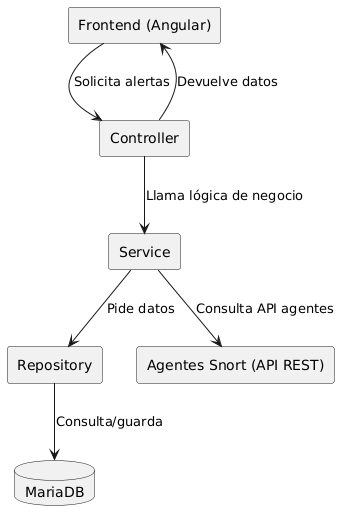
\includegraphics[width=0.5\textwidth]{documento/27.png}
	\caption{Flujo de funcionamiento del backend.}
	\label{fig:esquema-backend}
\end{figure}

\newpage

\subsection{Implementación del frontend}

El \textbf{frontend de R-Snort} se desarrolló como una \textbf{SPA (Single Page Application)} usando \texttt{Angular}, lo que proporciona una experiencia de usuario interactiva y fluida en el navegador, similar a una aplicación de escritorio. La interfaz está diseñada para que un administrador de seguridad pueda visualizar el estado de la red y configurar el sistema de detección de intrusos de forma unificada. A nivel de organización, la aplicación Angular se estructuró en distintos módulos o secciones, correspondientes a las funcionalidades principales: alertas, reglas, vista general (\texttt{overview}), estado del sistema y autenticación (\texttt{login}). Cada sección agrupa componentes, servicios y otros elementos específicos de esa funcionalidad, manteniendo el código modular y claro.

\subsubsection*{Módulos principales de la SPA}

\begin{itemize}
	\item \textbf{Login}: Maneja el proceso de autenticación de usuarios. Contiene el componente de inicio de sesión, donde se solicitan las credenciales. Al autenticarse correctamente, este módulo se encarga de almacenar el token JWT recibido y redirigir al usuario hacia la interfaz principal.
	
	\item \textbf{Overview (Vista general)}: Provee un tablero de control con estadísticas globales del sistema IDS. En esta sección se concentran visualizaciones resumidas de la información de seguridad, como gráficos de la cantidad de alertas por severidad a lo largo del tiempo, distribuciones de los tipos de alerta más frecuentes, protocolos más detectados, y otras métricas agregadas. Sirve para que el administrador obtenga de un vistazo el panorama de la actividad reciente en la red monitoreada.

	\begin{figure}[H]
		\centering
		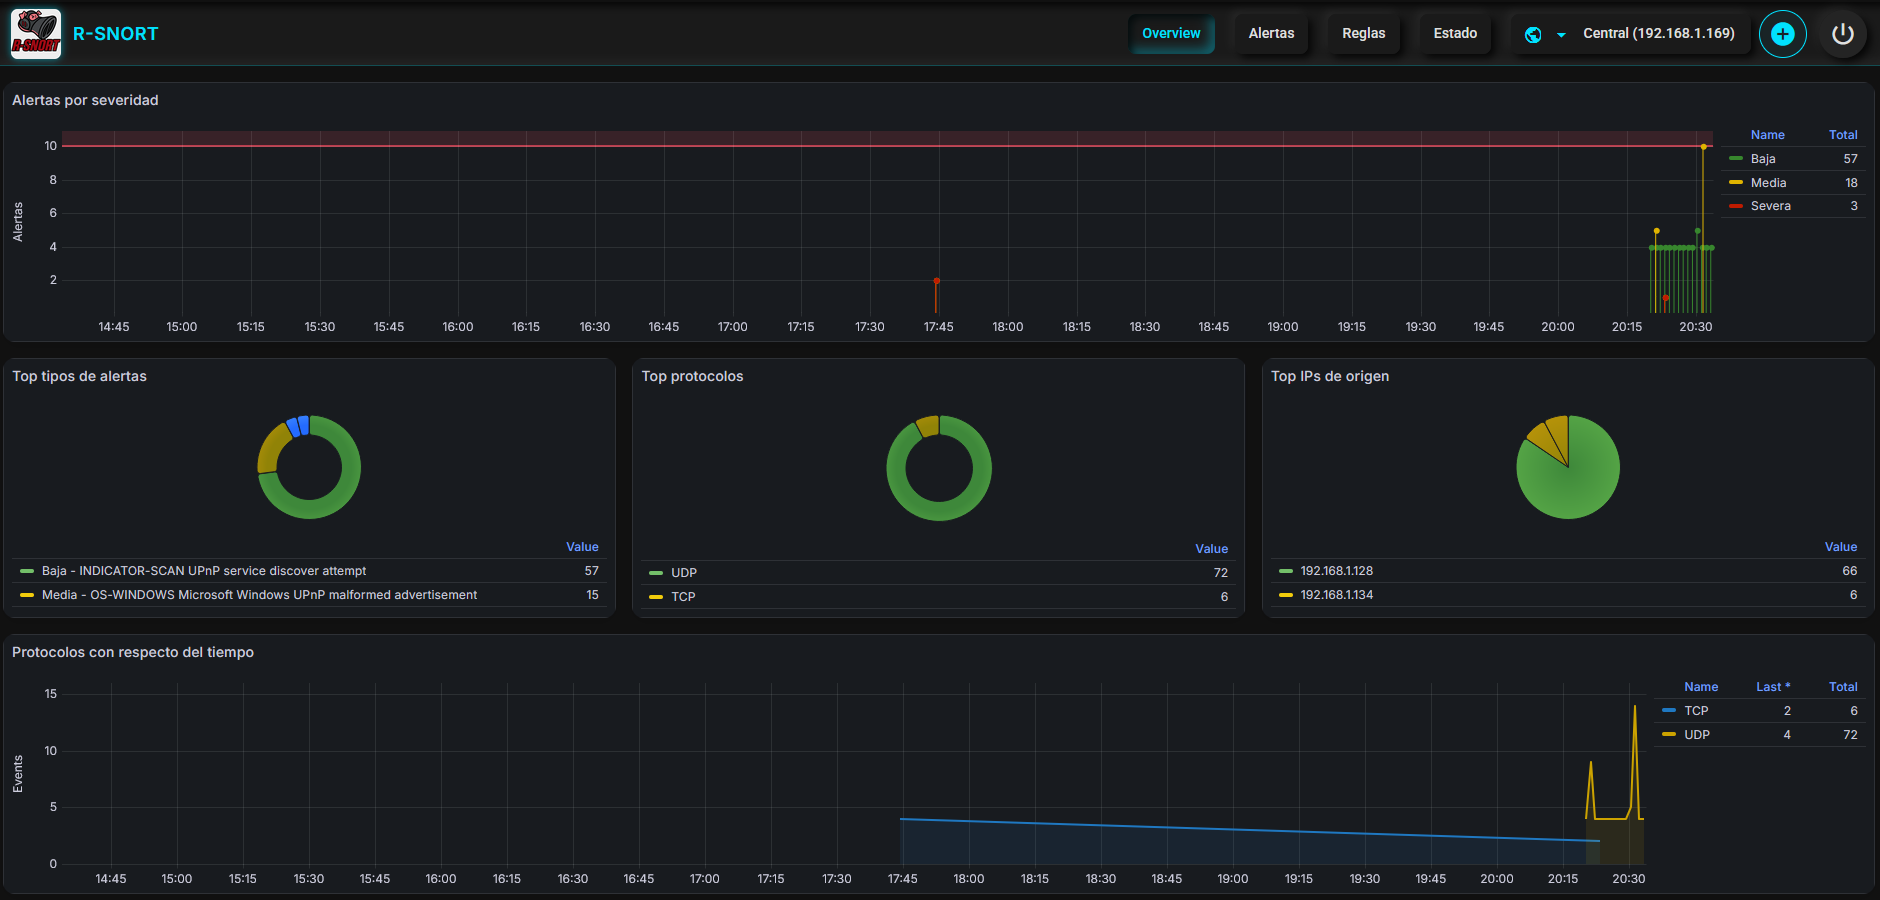
\includegraphics[width=0.9\textwidth]{documento/overview.png}
		\caption{Vista general.}
		\label{fig:overview-frontend}
	\end{figure}
	
	\item \textbf{Alertas}: Incluye los componentes para visualizar las alertas de seguridad provenientes de un agente seleccionado. Presenta un Panel de Alertas con indicadores numéricos de alertas por nivel de severidad (alta, media, baja) y una tabla con el listado de las últimas alertas detectadas con sus detalles (hora, tipo, origen, destino, etc.). Además, provee acciones para exportar datos, como botones para ``Descargar alertas de este agente'' o ``Descargar todas las alertas'' en formato CSV, facilitando el análisis externo de los eventos.
	
	\begin{figure}[H]
		\centering
		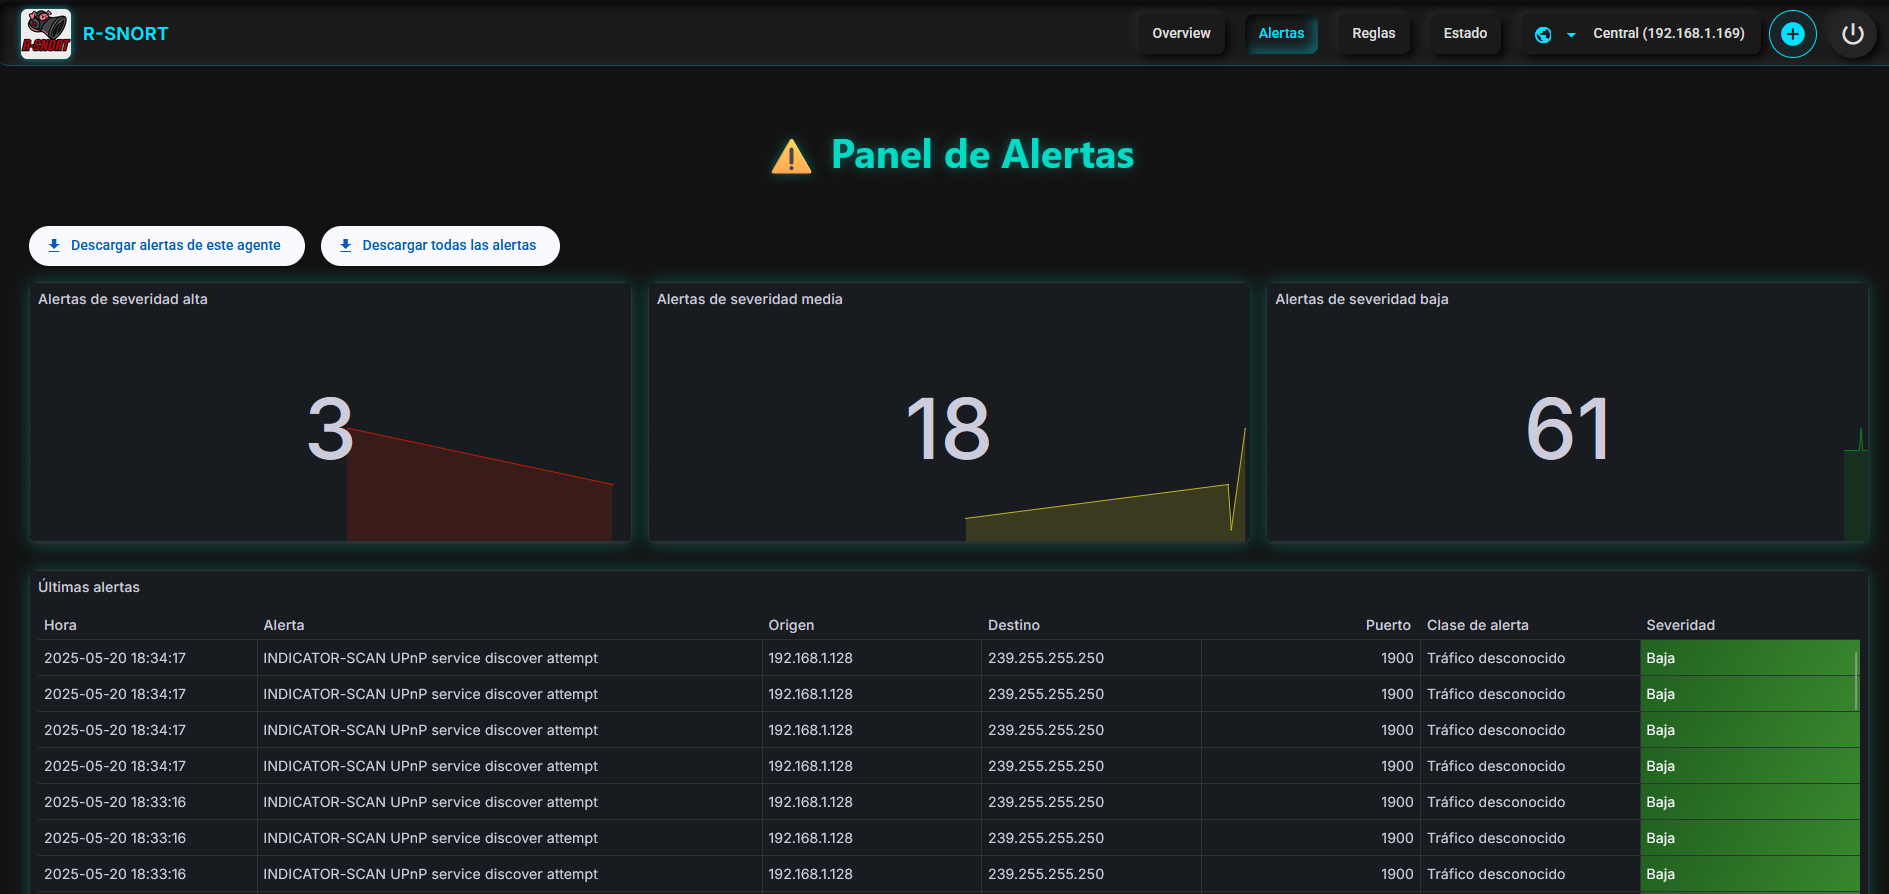
\includegraphics[width=0.9\textwidth]{documento/alertas.png}
		\caption{Vista de alertas del agente seleccionado en la interfaz R-Snort.}
		\label{fig:alertas-frontend}
	\end{figure}
	
	\item \textbf{Reglas}: Ofrece la interfaz para gestionar reglas de Snort de forma centralizada. Un componente de este módulo permite agregar una nueva regla mediante un formulario donde el usuario escribe la regla en formato Snort (texto), y enviarla al backend. Las reglas personalizadas existentes se muestran en una lista, incluyendo su \texttt{SID} (identificador), mensaje descriptivo y el contenido de la regla, con la opción de eliminarlas individualmente mediante un ícono de papelera. Si la regla no cuenta con la sintaxis correcta es rechazada.
	
	\begin{figure}[H]
		\centering
		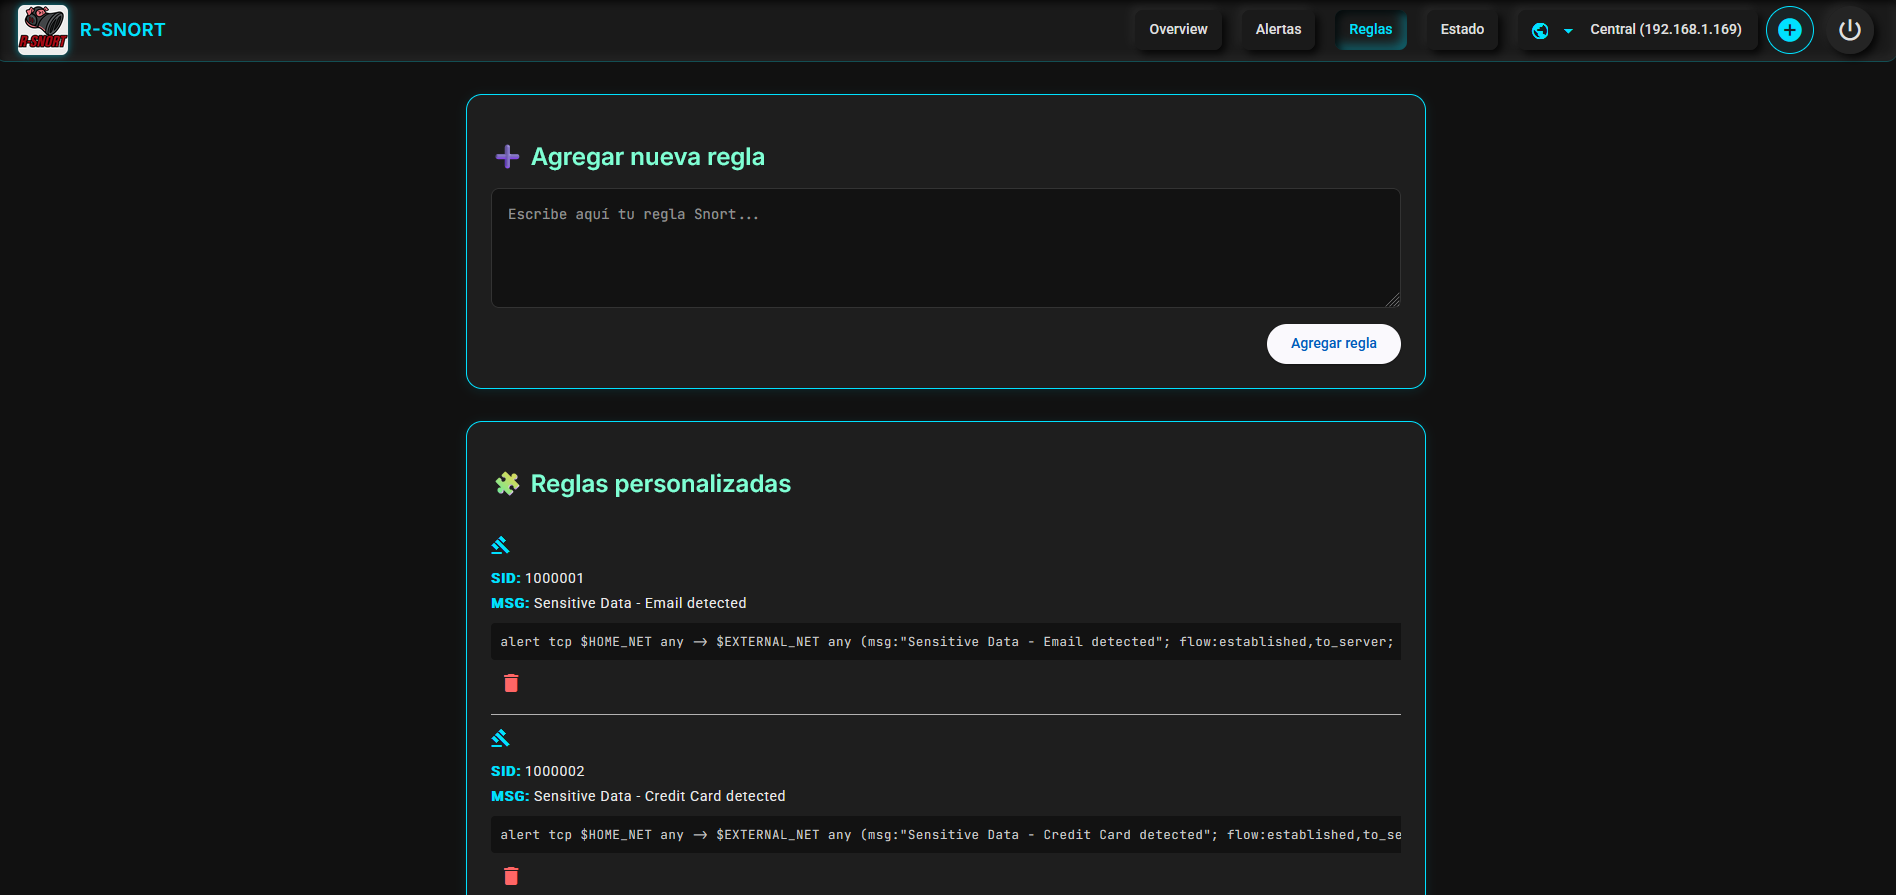
\includegraphics[width=0.9\textwidth]{documento/reglas.png}
		\caption{Reglas del sistema de R-Snort.}
		\label{fig:reglas-frontend}
	\end{figure}
	
	\item \textbf{Estado}: Muestra información en tiempo real del estado operativo tanto del agente seleccionado como del sistema central. Incluye gráficos de métricas del sistema (por ejemplo, temperatura de la CPU, uso de CPU y disco) y paneles de estado que indican si los servicios del agente están activos. También se presentan botones para reiniciar procesos como Snort (``Reiniciar Snort'') y una lista de logs archivados disponibles para descarga.
	
	\begin{figure}[H]
		\centering
		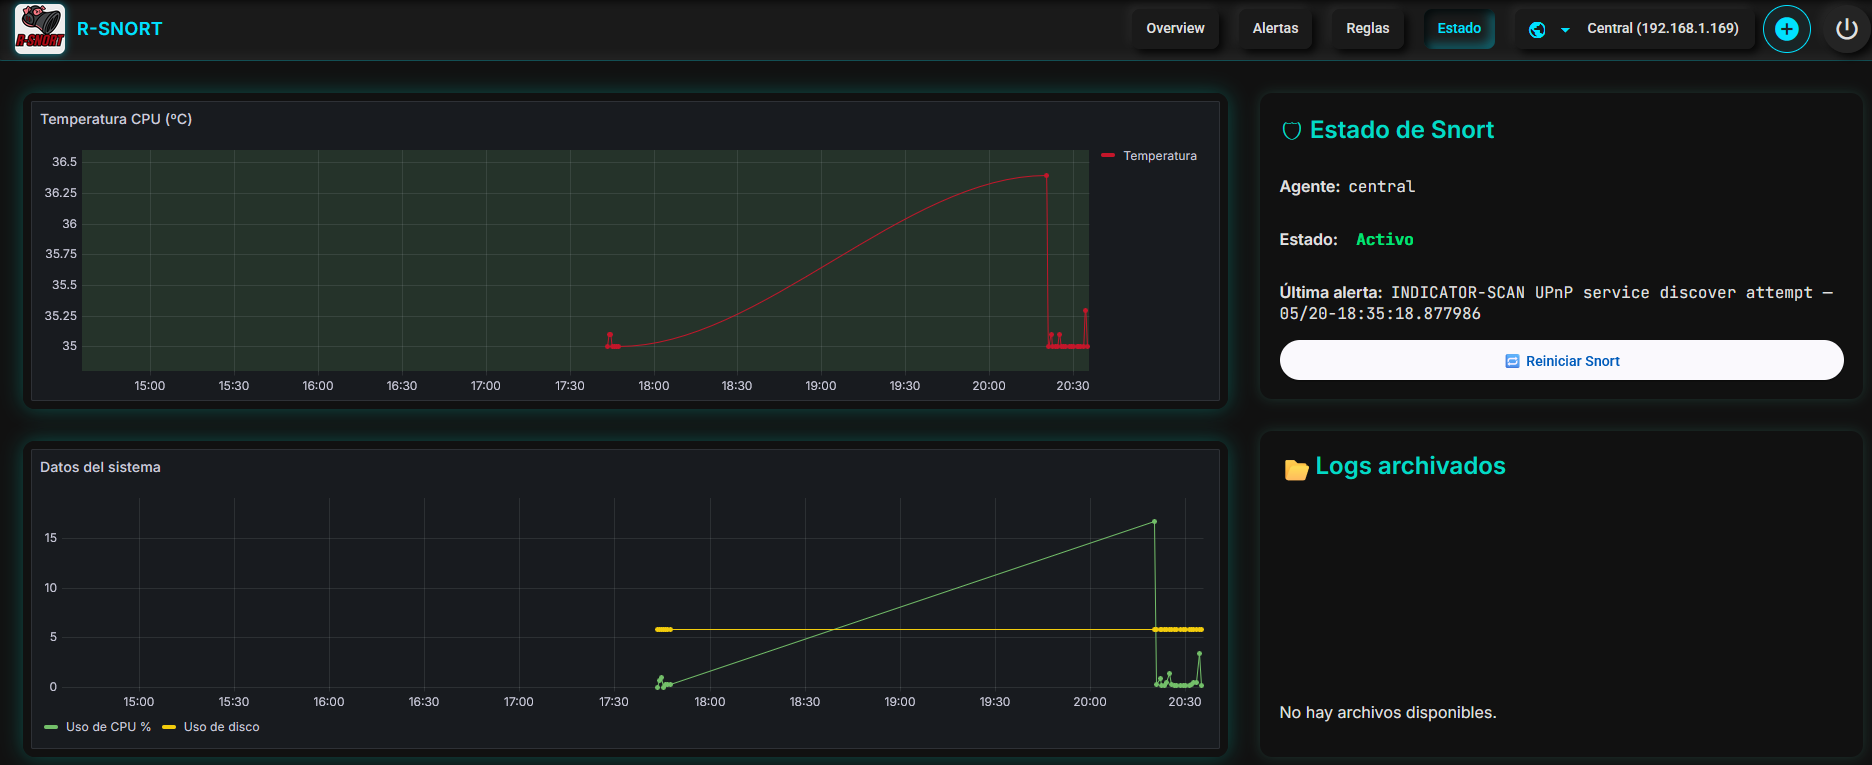
\includegraphics[width=0.9\textwidth]{documento/estado.png}
		\caption{Estado del agente seleccionado.}
		\label{fig:status-frontend}
	\end{figure}
	
		\begin{figure}[H]
		\centering
		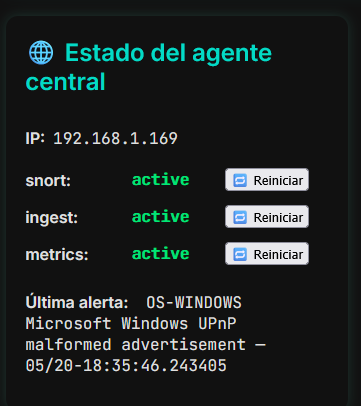
\includegraphics[width=0.6\textwidth]{documento/estado_agente.png}
		\caption{Estado de los servicios de un agente individual.}
		\label{fig:status-agent-frontend}
	\end{figure}
\end{itemize}

Además de estos módulos principales, la aplicación cuenta con componentes auxiliares como un \textbf{header} (encabezado) que contiene el menú de navegación y el selector de agente, \textbf{servicios compartidos} (por ejemplo, servicios para hacer peticiones HTTP al backend central, manejo del token JWT, etc.), \textbf{guards e interceptors}, y elementos de UI reutilizables (diálogos de confirmación, notificaciones, \texttt{pipes} para formateo, etc.). Toda esta estructura sigue la conveniencia de Angular de separar responsabilidades: \textbf{componentes} para la presentación, \textbf{servicios} para la lógica de datos/comunicación, y \textbf{guardas/interceptores} para control de flujo y seguridad en la interfaz.

\subsubsection{Enrutamiento y selección dinámica de agentes}

La SPA Angular define un sistema de rutas (\textit{routing}) para navegar entre las distintas secciones (\texttt{login}, \texttt{overview}, \texttt{alertas}, \texttt{reglas}, \texttt{estado}). Cada ruta está asociada a un componente principal de los mencionados módulos. Por ejemplo, se configuran rutas como \texttt{/login} para la pantalla de autenticación, \texttt{/overview} para la vista general, \texttt{/alertas} para el panel de alertas, etc. Una vez autenticado el usuario, navegar entre estas rutas no provoca recarga de la página, sino que Angular se encarga de cargar dinámicamente el componente correspondiente dentro de la misma aplicación.\newline

Un requerimiento particular de R-Snort es la capacidad de visualizar información de múltiples agentes de forma centralizada. Esto se resuelve en la interfaz mediante un mecanismo de \textbf{selección dinámica de agentes}. En la parte superior derecha de la aplicación (ver figuras), el usuario dispone de un menú desplegable que lista los agentes registrados. El usuario puede cambiar el agente activo seleccionándolo en ese menú, con lo cual la aplicación actualiza la información mostrada en todos los módulos (\texttt{alertas}, \texttt{reglas}, \texttt{overview}, \texttt{estado}) para reflejar los datos de ese agente.\newline

Se pretende manejar la selección de agente mediante un \textbf{servicio global} de Angular (por ejemplo, un \texttt{AgentService} que almacena el agente seleccionado en memoria). En este enfoque, las rutas no cambian cuando se selecciona otro agente; más bien, los componentes consultan al \texttt{AgentService} para saber qué agente utilizar en sus peticiones. Un cambio en la selección actualizaría dicho servicio y los componentes reaccionarían (por ejemplo, recargando datos). Esta aproximación evita tener parámetros en todas las rutas, a costa de no tener una URL única por agente (pero dado que el objetivo es administración interactiva, eso no suele ser un problema).\newline

En la implementación de R-Snort se ha optado por la comodidad de poder cambiar de agente sin recargar la aplicación. Al iniciar sesión, típicamente se selecciona un agente por defecto (por ejemplo, el agente \texttt{"central"}) para mostrar. Luego, al elegir otro agente en el menú desplegable, la aplicación realiza internamente las solicitudes al backend central para ese agente y actualiza las vistas. Todos los componentes clave (\texttt{alertas}, \texttt{reglas}, \texttt{estado}, etc.) están preparados para reaccionar ante un cambio de agente y volver a cargar sus datos desde el servidor central.\newline

El sistema de rutas de Angular también incorpora \textbf{guardas (guards)} para restringir el acceso a ciertas rutas. En particular, se utiliza un \textbf{guardia de autenticación} que impide el acceso a las rutas de la aplicación principal (\texttt{overview}, \texttt{alertas}, etc.) si el usuario no ha iniciado sesión. Esto se configura de forma que, si Angular detecta que no hay un token JWT válido almacenado (o que el usuario no ha pasado por login), automáticamente redirige la navegación hacia la ruta \texttt{/login}. A continuación se muestra un ejemplo simplificado de un \texttt{guard} de autenticación:

\begin{lstlisting}[language=Java, caption={Ejemplo simplificado de authGuard}, label={lst:authGuard}]
// Ejemplo de AuthGuard en Angular
@Injectable({ providedIn: 'root' })
export class AuthGuard implements CanActivate {
	constructor(private authService: AuthService, private router: Router) {}
	canActivate(): boolean {
		if (!this.authService.isLoggedIn()) {
			this.router.navigate(['/login']);
			return false;
		}
		return true;
	}
}

\end{lstlisting}

En el código anterior, el guard (\texttt{AuthGuard}) consulta a un servicio de autenticación \texttt{AuthService} para verificar si el usuario está logueado. El método \texttt{isLoggedIn()} típicamente comprueba si existe un \texttt{JWT} almacenado y vigente. Si no lo está, se realiza un \texttt{redirect} a la página de login y se bloquea la activación de la ruta solicitada; si sí lo está, se permite el acceso. Este guard se aplica, por ejemplo, a todas las rutas bajo \texttt{/agents/*} o a un grupo de rutas definidas para la parte protegida de la app.\newline

Asimismo, para hacer transparente el uso del JWT en el frontend, se ha implementado un \textbf{interceptor HTTP}. Este interceptor global intercepta todas las peticiones HTTP salientes desde Angular hacia el backend central y añade automáticamente la cabecera \texttt{Authorization: Bearer <token>} con el JWT que fue almacenado tras el login. De esta manera, los componentes y servicios del frontend no tienen que preocuparse de adjuntar manualmente el token en cada llamada; el interceptor garantiza que el backend reciba el token en cada petición, manteniendo la sesión autenticada.\newline

Si el token expirara o fuera inválido, el backend responderá con un error de no autorizado, y en respuesta la aplicación podría redirigir al usuario al login nuevamente. Esta lógica puede manejarse también en el interceptor o en un manejador centralizado de respuestas.

\subsubsection{Integración de Grafana para visualización de métricas}

Una característica destacada de R-Snort es la integración de paneles de \textbf{Grafana} en la interfaz web para mostrar \textbf{gráficos y métricas en tiempo real}. Grafana es una herramienta especializada en visualización de datos de monitorización, y su uso permite aprovechar gráficos interactivos sin tener que implementarlos desde cero.\newline

En el contexto de R-Snort, se ha utilizado Grafana para representar principalmente las métricas de rendimiento del sistema y \textbf{series temporales de las alertas}.

\subsubsection{Integración de Grafana en la interfaz Angular}

La integración técnica con Grafana se realiza mediante la inserción de sus dashboards en la página Angular, aprovechando la opción de \textbf{Iframes embebidos} de Grafana que permite compartir paneles mediante URLs especiales. En R-Snort, se utilizan \texttt{iframes} en los componentes Angular (como \texttt{OverviewComponent}) para incrustar paneles específicos. Por ejemplo, un \texttt{<iframe>} puede apuntar a una URL compartida por Grafana que renderiza únicamente la gráfica en modo \texttt{kiosk}, sin menús ni cabecera. Este método es sencillo y permite mostrar los datos en tiempo real sin complejidad adicional en el frontend.\newline

En cuanto a la \textbf{autenticación}, Grafana puede configurarse con acceso anónimo de solo lectura o mediante \texttt{API Keys} incrustadas en la URL. En R-Snort, se ha garantizado que el acceso a los gráficos esté restringido de forma segura (por ejemplo, corriendo Grafana localmente o con un usuario de sólo visualización). Cuando el usuario entra en las vistas \texttt{Overview} o \texttt{Estado}, los gráficos se cargan automáticamente según el agente seleccionado, ya sea modificando el \texttt{iframe} o pasando variables dinámicas a Grafana.\newline

Este tipo de integración aporta valor visual al frontend con mínimo esfuerzo, permitiendo combinar datos detallados con visualizaciones agregadas en una sola interfaz unificada.

\subsubsection{Ejemplo de interacciones en el frontend}

A continuación se muestran ejemplos representativos del funcionamiento del frontend.

\paragraph{Login y almacenamiento del token JWT}

Cuando el usuario inicia sesión, el token JWT es recibido y almacenado, y se redirige a la vista principal:

\begin{lstlisting}[language=Java, caption={Login y navegación tras autenticación}, label={lst:frontend-login}]
	this.authService.login(this.username, this.password).subscribe({
		next: () => this.router.navigate(['/overview']),
		error: () => this.loginError = true
	});
\end{lstlisting}

\paragraph{Carga de alertas del agente seleccionado}

El componente de alertas carga las alertas desde el backend, pasando el ID del agente seleccionado:

\begin{lstlisting}[language=Java, caption={Carga de alertas desde el servicio}, label={lst:frontend-alertas}]
	this.alertService.getAlertas(this.agenteSeleccionado.id).subscribe(alertas => {
		this.alertas = alertas;
	});
\end{lstlisting}

Gracias al \textbf{interceptor HTTP}, el token JWT es incluido automáticamente en la cabecera \texttt{Authorization} de cada petición, por lo que los componentes no necesitan preocuparse por ello.

\subsubsection{Resumen del frontend}

En síntesis, el frontend de R-Snort proporciona una interfaz SPA modular, fluida y responsiva que permite:

\begin{itemize}
	\item Navegar entre módulos como \texttt{alertas}, \texttt{reglas}, \texttt{estado} o \texttt{overview} sin recarga.
	\item Cambiar entre agentes en tiempo real mediante un selector global.
	\item Consultar alertas, gestionar reglas y visualizar métricas de forma centralizada.
	\item Integrar paneles de Grafana para enriquecer la experiencia visual.
	\item Proteger rutas con \textbf{guards} y mantener autenticación mediante JWT.
\end{itemize}

Esto permite al usuario controlar múltiples sensores Snort desde una única interfaz, combinando vistas detalladas (tablas de alertas o reglas) con paneles gráficos y opciones de administración remota.

\begin{figure}[htb]
	\centering
	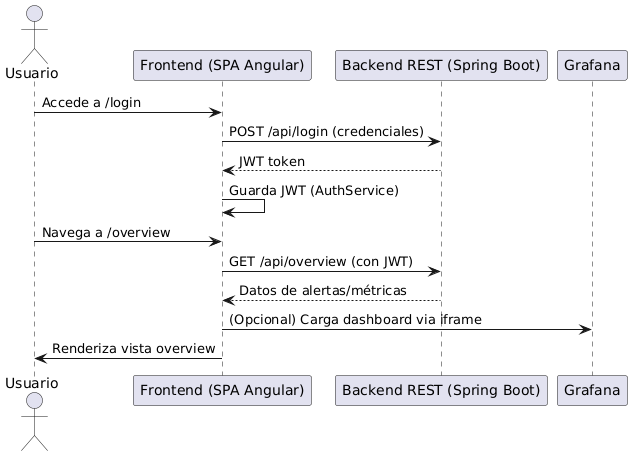
\includegraphics[width=0.8\textwidth]{documento/28.png}
	\caption{Diagrama de secuencia de interacción.}
	\label{fig:diagrama-secuencia-frontend}
\end{figure}

\section{Script automático R-Snort}

El sistema R-Snort se estructura en torno a dos componentes principales: el \texttt{snort-agent}, encargado de desplegar un nodo completo de detección de intrusiones en cada dispositivo monitorizado, y el \texttt{r-snort-central-module}, que actúa como módulo central de gestión y visualización. A continuación se describe en detalle el funcionamiento del instalador \texttt{snort-agent} y sus peculiaridades técnicas.

\subsection{Instalador del agente: \texttt{snort-agent}}

El script \texttt{snort-agent} automatiza la instalación y configuración de un agente R-Snort sobre sistemas Debian/Ubuntu con una instancia de Snort versión 3 ya sea con la configuración por defecto o personalizada, la base de datos local, servicios de monitorización REST y la integración con Grafana. El instalador está compuesto por varios scripts Bash y módulos Python que permiten que el agente funcione de forma autónoma tras su ejecución. El objetivo del instalador automático desde un principio se centra en usuarios con poco conocimiento técnico haciéndolo prácticamente plug and play.

\paragraph{Script \texttt{00\_common.sh:}} Este script inicial crea la estructura de configuración del agente, incluyendo:

\begin{itemize}
	\item Generación de un identificador \texttt{UUID} persistente para identificar únicamente al agente.
	\item Creación de archivos de entorno (\texttt{db.cnf}, \texttt{env.sh} y \texttt{env.service}) que almacenan credenciales y configuración necesaria para el resto de scripts y servicios.
\end{itemize}

\begin{lstlisting}[language=bash, caption={Fragmento de creación del archivo db.cnf}]
	cat >"$DB_CNF" <<EOF
	[client]
	user=$DB_USER
	password=$DB_PASS
	database=$DB_NAME
	host=127.0.0.1
	EOF
\end{lstlisting}

\paragraph{Script \texttt{01\_install\_db.sh:}} Este script instala MariaDB y crea el esquema de base de datos para las alertas y métricas. Las tablas \texttt{alerts} y \texttt{system\_metrics} permiten almacenar información relevante como el origen/destino del ataque, el tipo de alerta, el uso de CPU, entre otros.

\paragraph{Script \texttt{02\_configure\_snort.sh:}} Configura Snort para ejecutarse como servicio en segundo plano, escaneando el tráfico de red a través de la interfaz detectada automáticamente. También modifica el archivo \texttt{snort.lua} para incluir la salida \texttt{alert\_json} y define un servicio \texttt{systemd}. Una particularidad es que el script escoge la interfaz activada en modo promiscuo para la tarea de escuchar el tráfico de red, en caso de no haber ninguna interfaz en dicho modo escogerá escuchar a través de la interfaz usada originalmente por Snort.

\begin{lstlisting}[language=bash, caption={Definición del servicio systemd para Snort}]
	[Service]
	ExecStart=/usr/local/snort/bin/snort -q -c /usr/local/snort/etc/snort/snort.lua -i $IFACE -A alert_json -l /opt/snort/logs/live
	Restart=always
\end{lstlisting}

\paragraph{Script \texttt{03\_log\_rotation.sh:}} Implementa un mecanismo de rotación de logs usando logrotate, que evita el crecimiento descontrolado del archivo \texttt{alert\_json.txt}. Además, se configura un \texttt{cron job} para archivado diario de logs.

\paragraph{Script \texttt{04\_setup\_grafana.sh:}} Automatiza la instalación de Grafana, habilita el modo anónimo y crea un token de autenticación mediante un Service Account. El script es especialmente estable, incluyendo comprobaciones de salud, reintentos y validaciones en cada paso aguantando desfases que pueden ser provocados por equipos muy lentos o muy rápidos.

\paragraph{Script \texttt{05\_setup\_python\_env.sh:}} Crea un entorno virtual de Python donde se instalan dependencias como \texttt{FastAPI}, \texttt{PyMySQL}, \texttt{requests} y \texttt{psutil}. Esto aísla el entorno de ejecución de posibles conflictos con paquetes del sistema.

\paragraph{Script \texttt{06\_install\_services.sh:}} Copia los scripts Python al destino final y registra tres servicios principales:

\begin{itemize}
	\item \textbf{rsnort-api.service:} expone una API REST basada en FastAPI para interactuar con el agente.
	\item \textbf{rsnort-ingest.service:} lee continuamente el archivo \texttt{alert\_json.txt} y vuelca su contenido en la base de datos.
	\item \textbf{rsnort-metrics.timer:} ejecuta un script cada 30 segundos para capturar métricas del sistema.
\end{itemize}

\paragraph{Script \texttt{07\_import\_dashboard.sh:}} Importa automáticamente un dashboard preconfigurado en Grafana, lo vincula con el datasource \texttt{Snort-MariaDB} y proporciona una visualización inmediata y profesional de alertas y métricas.

\paragraph{Scripts Python: arquitectura y lógica interna}

\begin{itemize}
	\item \textbf{\texttt{agent\_api.py}:} implementa endpoints REST para acceder a alertas, métricas, reglas activas, archivos archivados y gestión de servicios. Incluye validación sintáctica de reglas antes de ser añadidas.
	\item \textbf{\texttt{ingest\_service.py}:} monitoriza el archivo \texttt{alert\_json.txt} detectando rotaciones y evita duplicados usando un hash de línea.
	\item \textbf{\texttt{metrics\_timer.py}:} calcula la carga de CPU, uso de RAM, espacio en disco y temperatura media del sistema. Esta última es estimada si los sensores no están disponibles.
\end{itemize}

\begin{lstlisting}[language=Python, caption={Fragmento de inserción de alerta en ingest\_service.py}]
	def insert_alert(rec):
	ts_original = rec.get("timestamp", "")
	ts_normalizado = normalize_ts(ts_original)
	rec["timestamp"] = ts_normalizado
	...
	cur.execute("""
	INSERT INTO alerts (...)
	VALUES (%s, ..., %s)
	""", valores + [AGENT_ID])
\end{lstlisting}

\begin{figure}[H]
	\centering
	 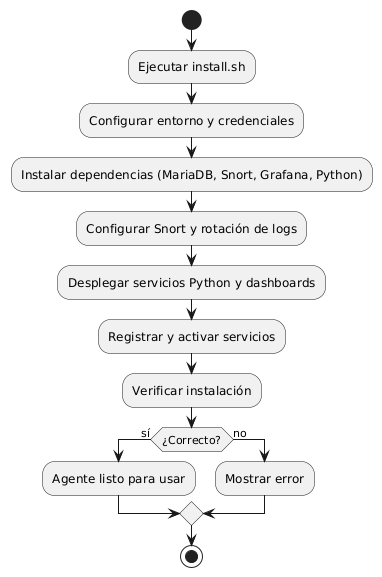
\includegraphics[width=0.45\textwidth]{documento/29.png}
	\caption{Proceso detallado de instalación del agente R-Snort.}
	\label{fig:bpmn-snort-agent}
\end{figure}

% --- Parte del agente ya desarrollada arriba ---

\subsection{Instalador del módulo central: \texttt{r-snort-central-module}}

El módulo central constituye el componente principal del proyecto, este se encagar de llevar a cabo la gestión y visualización del sistema R-Snort con todo lo que ello conlleva. Permite consolidar alertas y métricas provenientes de múltiples agentes, así como gestionar reglas, usuarios y agentes desde una interfaz web integrada. Este componente fusiona un backend en Spring Boot con un frontend en Angular, y se despliega como un servicio \texttt{systemd}.

\paragraph{Script \texttt{00\_common.sh:}} Define rutas comunes, credenciales de base de datos y funciones auxiliares como la detección de IP local. Estos valores se reutilizan en todos los demás scripts.

\paragraph{Script \texttt{01\_dependencies.sh:}} Instala dependencias clave del sistema:
\begin{itemize}
	\item \textbf{Java JDK 17 y Maven}, necesarios para compilar el backend.
	\item \textbf{Node.js 18 y Angular CLI}, requeridos para construir el frontend.
	\item Herramientas auxiliares como \texttt{git}, \texttt{curl} y \texttt{apache2-utils}.
\end{itemize}

\paragraph{Script \texttt{02\_compile\_frontend.sh:}} Inyecta automáticamente la IP local del backend en los archivos de entorno de Angular, compila la aplicación en modo producción, y copia los archivos resultantes al directorio estático del backend para que se empaqueten en el JAR final.

\paragraph{Script \texttt{03\_compile\_backend.sh:}} Compila el backend con Maven (o su wrapper si está disponible), generando un archivo \texttt{rsnort.jar} que incluye también el frontend. Este archivo se copiará posteriormente a \texttt{/opt/rsnort-backend/}.

\paragraph{Script \texttt{04\_prepare\_db.sh:}} Garantiza la existencia de la tabla \texttt{users} en la base de datos, la cual almacena credenciales, roles y estados de activación de los usuarios que acceden a la interfaz web.

\paragraph{Script \texttt{05\_add\_admin\_user.sh:}} Solicita por terminal el correo y contraseña del primer administrador, genera un \texttt{hash bcrypt} con \texttt{htpasswd}, e inserta el usuario directamente en la tabla \texttt{users}.

\paragraph{Script \texttt{06\_setup\_agents.sh:}} Permite definir los agentes registrados en el sistema. Se crea el archivo \texttt{agents.json} en \texttt{/var/lib/rsnort-backend/}, incluyendo el agente central (automático) y cualquier otro agente remoto adicional que se desee agregar.

\paragraph{Script \texttt{07\_install\_services.sh:}} Este script empaqueta y despliega el sistema como servicio:
\begin{itemize}
	\item Copia el JAR generado a \texttt{/opt/rsnort-backend/}.
	\item Define variables de entorno tanto para \texttt{systemd} como para shells interactivos.
	\item Crea un servicio \texttt{rsnort-backend.service} que lanza el backend con Java y asegura su persistencia.
\end{itemize}

\begin{lstlisting}[language=bash, caption={Fragmento del servicio systemd para el backend}]
	[Service]
	ExecStart=/usr/bin/java -jar /opt/rsnort-backend/rsnort.jar
	EnvironmentFile=/etc/rsnort-backend/rsnort.env
	Restart=on-failure
	ProtectSystem=full
	PrivateTmp=true
\end{lstlisting}

\paragraph{Script \texttt{run\_all.sh:}} Pone en marcha todos los pasos anteriores con mensajes en color y ejecución secuencial para que el usuario final sea capaz de visualizar el estado de la instalación. Ejecuta cada script con los permisos adecuados (algunos como usuario regular, otros como root) y resume el proceso al finalizar proporcionando instrucciones de acceso.

\begin{figure}[H]
	\centering
	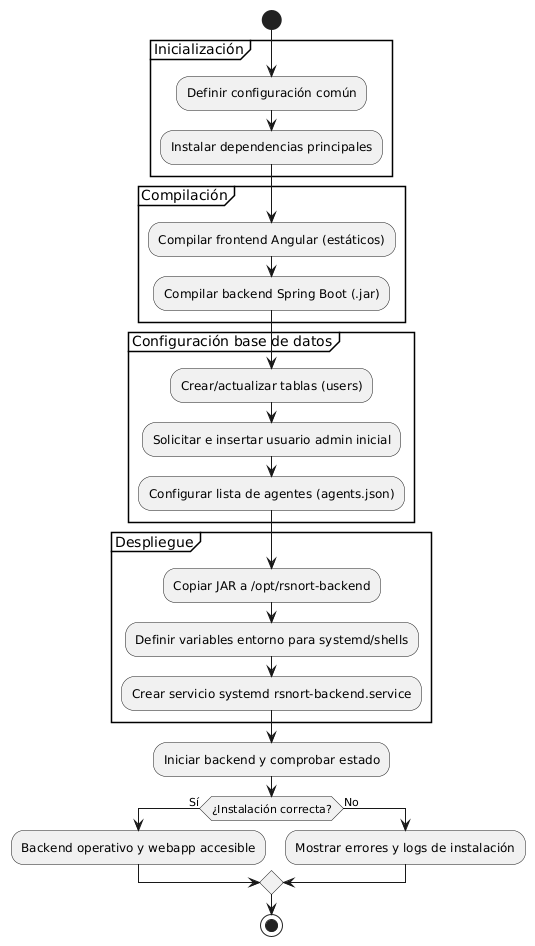
\includegraphics[width=0.57\textwidth]{documento/30.png}
	\caption{Proceso escalonado de instalación del módulo central de R-Snort.}
	\label{fig:bpmn-snort-central}
\end{figure}

Este instalador permite desplegar un sistema de visualización y control, que centraliza alertas y datos de múltiples agentes, ofrece una interfaz segura para la administración de reglas y usuarios, y facilita el mantenimiento y la extensión futura del sistema R-Snort.


\clearpage
\null
\thispagestyle{empty}
\newpage
\chapter{Caso práctico: utilización del frontend de R-Snort}

El sistema R-Snort se ha desplegado y evaluado en un entorno realista orientado a redes domésticas avanzadas o pequeñas oficinas (SOHO), simulando un entorno distribuido de múltiples subredes monitorizadas mediante instancias independientes de Snort 3 en Raspberry Pi 5.

\section{Entorno de trabajo}

La Figura~\ref{fig:esquema-red} muestra el esquema general del entorno de pruebas. En este escenario, se distingue un módulo central encargado de consolidar alertas, métricas y reglas, así como otro agente perteneciente a otra subred, cada uno conectado a un switch con funcionalidad de \textit{port mirroring}. Esto permite clonar todo el tráfico de la red al puerto monitorizado, donde se encuentra instalado Snort en cada caso.

\begin{figure}[H]
	\centering
	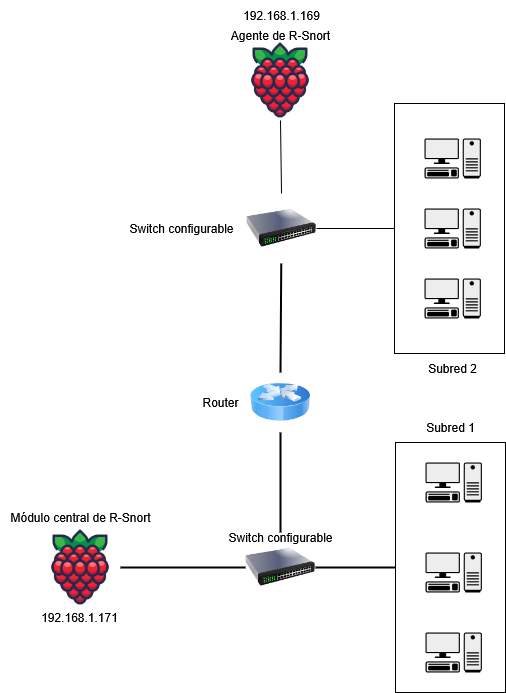
\includegraphics[width=0.65\textwidth]{documento/esquema_red.png}
	\caption{Esquema lógico de red con múltiples agentes Snort y módulo central R-Snort.}
	\label{fig:esquema-red}
\end{figure}

\newpage

El objetivo de esta distribución es comprobar la eficacia del proyecto en un entorno lo más cercano a una red PYME o SOHO, el agente con IP 192.168.1.169 se encarga de recoger las alertas de su subred asignada a través del port mirroring que copiará todo el tráfico de los demás puertos hacia el agente, de la misma manera, el módulo central recoge todo el tráfico de su correspondiente switch usando la misma técnica con la funcionalidad añadida de que el módulo central cuenta con el frontend previamente instalado que va a permitir cubrir toda la red de vigilancia.\newline

Aunque en la práctica solo se ha empleado un agente Snort por limitaciones de infraestructura (dos si contamos el módulo central), el diseño y la implementación del sistema permiten escalar horizontalmente con facilidad, añadiendo nuevos agentes usando el instalador automático de snort-agent, posteriormente agregando la IP del nuevo agente mediante la interfaz del módulo central.\newline

El hardware empleado para el despliegue y validación del sistema R-Snort incluye los siguientes dispositivos y componentes de red:

\begin{itemize}
	\item \textbf{Raspberry Pi 5 (8 GB de RAM)} con \texttt{Ubuntu Server 22.04 LTS (aarch64)}. Esta placa actúa como \emph{módulo central} de R-Snort, alojando:
	\begin{itemize}
		\item Snort 3.1.84.0 compilado con Hyperscan.
		\item \texttt{rsnort-backend} (Spring Boot) y \texttt{rsnort-frontend} (Angular).
		\item Base de datos MariaDB para alertas, métricas y configuración.
		\item Grafana 12 para dashboards de rendimiento, alertas y uso de recursos.
		\item Servicios systemd: \texttt{rsnort-backend.service}.
	\end{itemize}
	Se conecta a un switch gestionable mediante un adaptador USB 3.0 → Gigabit para garantizar ancho de banda completo y latencia mínima en la ingesta de métricas.
	
	\item \textbf{Raspberry Pi 3 Model B (1 GB de RAM)} con \texttt{Ubuntu Server 22.04 LTS}. Funciona como \emph{agente} Snort, ejecutando:
	\begin{itemize}
		\item Snort 3.1.84.0 compilado con Hyperscan.
		\item Servicios systemd: \texttt{rsnort-ingest}, \texttt{rsnort-api}, \texttt{rsnort-metrics}.
		\item Configuración optimizada (NUMA deshabilitado, perfil ligero) para adaptarse a recursos limitados.
	\end{itemize}
	Está conectado al puerto mirror de un switch gestionable Tenda TEG205E (5 puertos Gigabit), que replica el tráfico de la subred al sensor.
	
	\item \textbf{Switch gestionable Tenda TEG205E} con port mirroring activado, replicando todo el tráfico ethernet de cada subred hacia el agente correspondiente sin afectar al tráfico productivo.
	
	\item \textbf{Dispositivos cliente heterogéneos} (Windows 11, Ubuntu Desktop), que generan tráfico de usuario real y ataques de prueba (p. ej. nmap, peticiones DNS, HTTP).
	
	\item \textbf{PC con Ubuntu Server 22.04 LTS (x86\_64)}. Solo se utiliza para pruebas puntuales (simulación de escenarios, análisis offline de logs, generación de tráfico controlado) y no forma parte del despliegue productivo.
\end{itemize}

Todos los componentes de R-Snort se comunican vía HTTP REST API en el puerto \texttt{9000}, intercambiando alertas y métricas con la base de datos central. Grafana 12, instalado en la Raspberry Pi 5, se conecta directamente a MariaDB para ofrecer dashboards interactivos de alertas, consumo de CPU/RAM y mapas de tráfico en tiempo real.

\section{Instalación del sistema}

El sistema R-Snort (abreviatura de \textit{Raspberry-Snort}) ha sido concebido como una solución ligera, modular y automatizada para proteger redes pequeñas o entornos de baja potencia, como los basados en dispositivos ARM (Raspberry Pi). Todos sus componentes han sido diseñados para ejecutarse sin dificultad en hardware con recursos limitados, sin renunciar a funcionalidades avanzadas de inspección y monitorización.\newline

Aunque R-Snort es plenamente compatible con cualquier sistema Ubuntu/Debian de arquitectura x86\_64 o ARM64, la elección de Raspberry Pi como plataforma principal responde al objetivo de validar su comportamiento en contextos realistas de bajo consumo, alta eficiencia energética y presupuesto reducido.\newline

El sistema completo se compone de tres grandes bloques:

\begin{itemize}
	\item \textbf{Instalador del complemento del TFG (R-Snort3):} encargado de desplegar automáticamente una instancia personalizada y optimizada de Snort versión 3, incluyendo todas las dependencias, configuraciones y adaptaciones necesarias para PYMES y redes SOHO.
	
	\item \textbf{Módulo de agente (\texttt{snort-agent}):} permite la captura y gestión local de alertas y métricas del sistema. Se comunica con el módulo central mediante una API REST y transmite datos a una base de datos que es leída por Grafana mediante un dashboard personalizado y adaptado a alertas de Snort 3 y métricas de sistemas Linux.
	
	\item \textbf{Módulo central (\texttt{rsnort-central-module}):} centraliza la gestión del sistema, permitiendo desde una interfaz web el control de reglas, la visualización de alertas, la integración con Grafana y la supervisión de múltiples agentes distribuidos.
\end{itemize}

En el contexto de este Trabajo Fin de Grado, el desarrollo se ha centrado principalmente en los dos últimos módulos, es decir, en la creación de una interfaz web completa, distribuida y funcional mediante \texttt{Spring Boot} (backend) y \texttt{Angular} (frontend), que permita interactuar con los agentes y gestionar Snort de forma remota.\newline

No obstante, para aprovechar al máximo las capacidades del sistema, se ha optado por utilizar la instancia personalizada de Snort 3 generada por el complemento del TFG, en lugar de emplear la versión genérica del IDS. Esta elección permite reducir el consumo de recursos, aumentar la compatibilidad con entornos ARM y facilitar la integración con los módulos del sistema.\newline

\textbf{Por tanto, como requisito previo a la instalación de los agentes, se asume que el sistema ya dispone de Snort 3 instalado correctamente}, ya sea mediante el complemento \texttt{R-Snort3} o a través de una instalación manual compatible. Las instrucciones siguientes parten de esa premisa.

\vspace{0.5cm}
\noindent \textbf{Tabla \thetable: Requisitos del sistema para el despliegue de R-Snort}
\begin{table}[H]
	\centering
	\begin{tabular}{|p{5.5cm}|p{8cm}|}
		\hline
		\rowcolor[HTML]{E0E0E0}
		\textbf{Tipo de requisito} & \textbf{Descripción} \\
		\hline
		\textbf{R1 - Requisito funcional} & El sistema debe disponer de Snort 3 previamente instalado y configurado correctamente. \\
		\hline
		\textbf{R2 - Requisito funcional} & El agente debe enviar alertas y métricas al módulo central mediante API REST. \\
		\hline
		\textbf{R3 - Requisito funcional} & El módulo central debe permitir visualizar alertas, editar reglas y gestionar agentes desde la web. \\
		\hline
		\textbf{R4 - Requisito funcional} & Los logs deben poder rotarse y almacenarse automáticamente para fines forenses. \\
		\hline
		\textbf{R5 - Requisito no funcional} & El sistema debe ejecutarse correctamente en hardware de bajo consumo como Raspberry Pi 3 o 5. \\
		\hline
		\textbf{R6 - Requisito no funcional} & La instalación debe estar automatizada y requerir intervención mínima del usuario. \\
		\hline
		\textbf{R7 - Requisito no funcional} & El sistema debe integrarse con MariaDB y Grafana sin configuraciones manuales complejas. \\
		\hline
		\textbf{R8 - Requisito no funcional} & La interfaz web debe ser accesible desde cualquier navegador moderno sin necesidad de complementos. \\
		\hline
	\end{tabular}
	\caption{Requisitos funcionales y no funcionales previos al despliegue del sistema R-Snort}
	\label{tab:requisitos-rsnort}
\end{table}

\subsection{Preparación de la instalación}

\subsubsection{Instalación del sistema operativo en las Raspberry Pi}

Antes de comenzar con la instalación del ecosistema R-Snort, es importante preparar adecuadamente el entorno de trabajo. Como se ha explicado previamente, R-Snort está pensado para ejecutarse en dispositivos de bajo consumo como las Raspberry Pi, aunque también es compatible con cualquier sistema Ubuntu/Debian.\newline

El primer paso consiste en instalar el sistema operativo en los dispositivos que actuarán como módulo central o como agentes de Snort. Para ello se utiliza \textbf{Raspberry Pi Imager}~\cite{raspberrypi_software}, una herramienta oficial y sencilla que permite seleccionar el modelo de Raspberry Pi, elegir la distribución de Linux deseada e instalarla automáticamente en una tarjeta microSD.\newline

En este caso, el sistema operativo elegido ha sido \texttt{Ubuntu Server 25.04 (64-bit)}, que ofrece un equilibrio excelente entre rendimiento, estabilidad y compatibilidad con las herramientas utilizadas por R-Snort.

\begin{figure}[H]
	\centering
	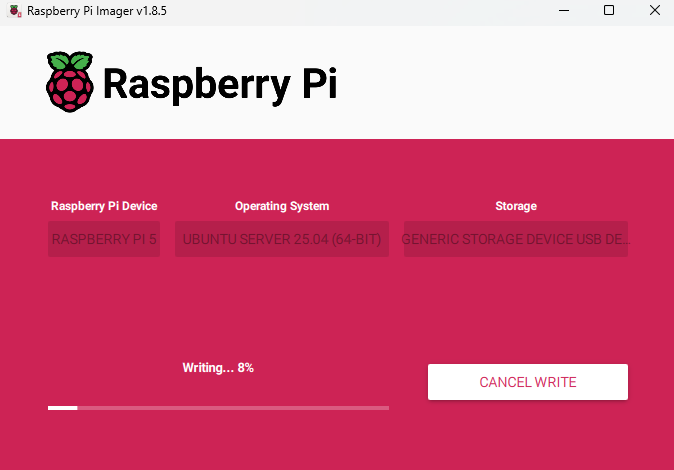
\includegraphics[width=0.8\textwidth]{install/1.png}
	\caption{Proceso de escritura de Ubuntu Server 25.04 (64-bit) en una Raspberry Pi 5 mediante Raspberry Pi Imager.}
	\label{fig:preparacion-sistema}
\end{figure}

\subsubsection{Conexiones físicas de la Raspberry Pi 5}

Una vez instalado el sistema operativo tanto en la \textbf{Raspberry Pi 5} (que actuará como módulo central) como en la \textbf{Raspberry Pi 3 Model B} (que funcionará como agente Snort), se procede a realizar las conexiones de red necesarias para cada una de ellas.\newline

En el caso de la Raspberry Pi 5, se conectan \textbf{dos interfaces de red físicas}. Esta decisión responde a la necesidad de separar el tráfico de administración del tráfico de monitorización. Por una parte, la interfaz principal \texttt{eth0} proporciona conectividad a internet y se utiliza para el control general del sistema. Por otra, se añade una segunda interfaz de red mediante adaptador USB Ethernet, configurada como \textbf{interfaz promiscua} y renombrada automáticamente como \texttt{enxc8a362b4a702}.\newline

Esta segunda interfaz está especialmente diseñada para capturar todo el tráfico de red redirigido mediante \textit{port mirroring} desde el switch gestionable. Por razones de seguridad, el script de instalación de la instancia personalizada de Snort 3 desarrollada en el complemento del TFG desactiva cualquier dirección IP en esta interfaz, dejándola exclusivamente dedicada a la escucha pasiva.

\begin{figure}[H]
	\centering
	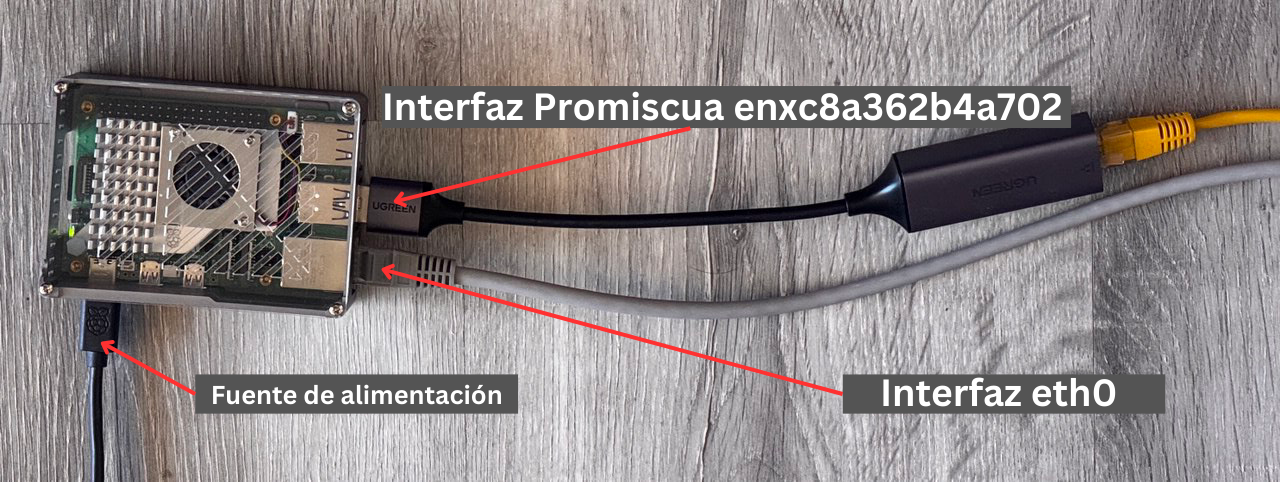
\includegraphics[width=0.8\textwidth]{install/0.1.png}
	\caption{Conexión física de la Raspberry Pi 5 como módulo central.}
	\label{fig:conexion-central-rpi5}
\end{figure}


\subsubsection{Configuración del switch y port mirroring}

En el switch gestionable Tenda, se han establecido las conexiones necesarias para habilitar la monitorización del tráfico de red. Por un lado, se conecta el router doméstico al puerto 1, lo que proporciona conectividad a internet a todos los dispositivos conectados al switch. Por otro lado, los puertos 2 y 3 se utilizan para conectar distintos dispositivos de la red local que generarán tráfico.\newline

La interfaz en modo promiscuo de la Raspberry Pi 5 se conecta al puerto 4 del switch mediante un adaptador USB a Ethernet. Esta interfaz será la encargada de recibir todo el tráfico replicado desde los demás puertos del switch.\newline

Para lograr este comportamiento, se configura la opción de \textit{port mirroring} desde la interfaz web del switch. Se establece el puerto 4 como destino del mirroring, y como fuente todos los puertos del 1 al 3, en ambas direcciones. Esta configuración garantiza que todo el tráfico entrante y saliente de los dispositivos conectados sea duplicado y enviado a la Raspberry Pi 5 para su análisis con Snort 3.

\begin{figure}[H]
	\centering
	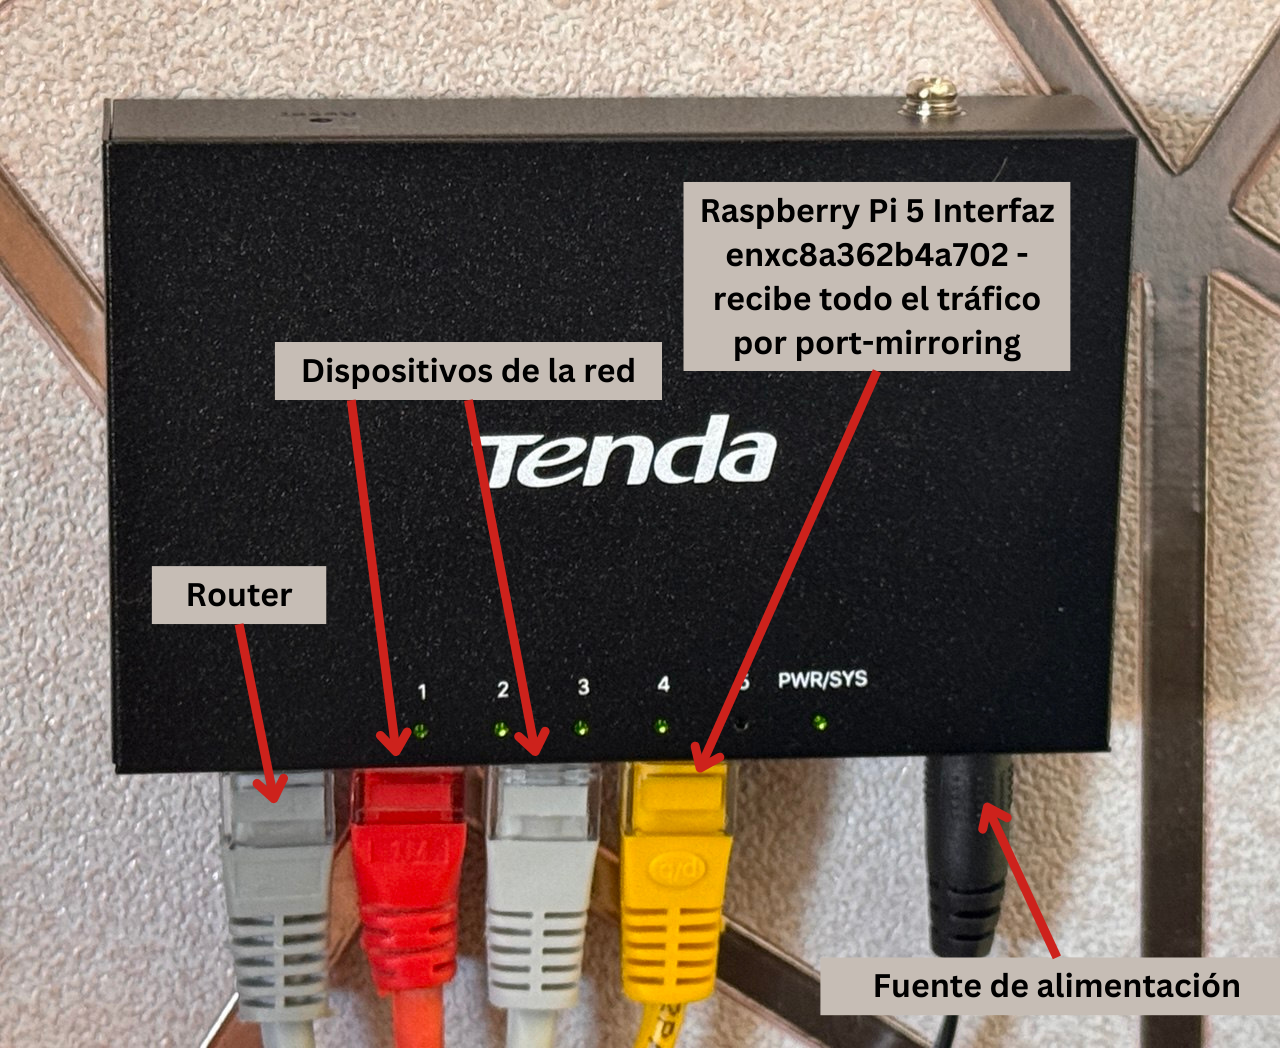
\includegraphics[width=0.6\textwidth]{install/0.2.png}
	\caption{Conexiones del switch.}
	\label{fig:switch-conexiones}
\end{figure}

\begin{figure}[H]
	\centering
	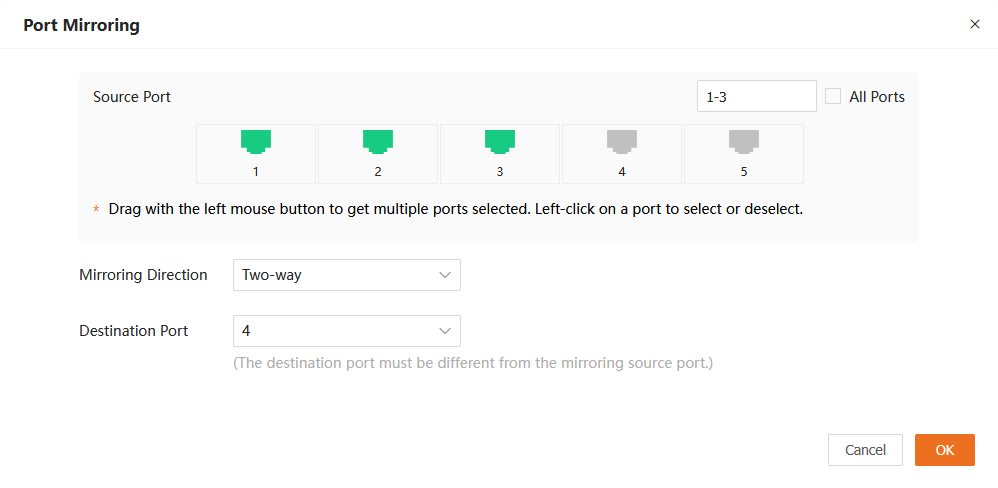
\includegraphics[width=0.70\textwidth]{install/9-asignacion_port.png}
	\caption{Configuración del mirroring.}
	\label{fig:switch-mirroring}
\end{figure}


\subsubsection{Conexión del agente en la subred secundaria}

La subred secundaria es gestionada por una \textbf{Raspberry Pi 3 Model B}, que actúa como agente Snort. Debido a las limitaciones del hardware, solo dispone de una interfaz de red física (\texttt{eth0}), la cual será utilizada simultáneamente como interfaz promiscua y como salida a internet.\newline

Aunque esta práctica no es recomendable en entornos de producción —donde se sugiere eliminar la dirección IP de la interfaz dedicada a la captura para evitar accesos no deseados— en este caso se ha considerado aceptable al tratarse de un entorno de pruebas controlado.\newline

El instalador del complemento de Snort 3 personalizado para PYMEs está diseñado para manejar estas situaciones. En sistemas con múltiples interfaces, pregunta al usuario si desea borrar la IP de la interfaz promiscua, evitando así riesgos innecesarios. Sin embargo, si solo se detecta una interfaz, como en esta Raspberry Pi 3, la lógica del script omite esa pregunta para prevenir una pérdida accidental de conectividad.

\begin{figure}[H]
	\centering
	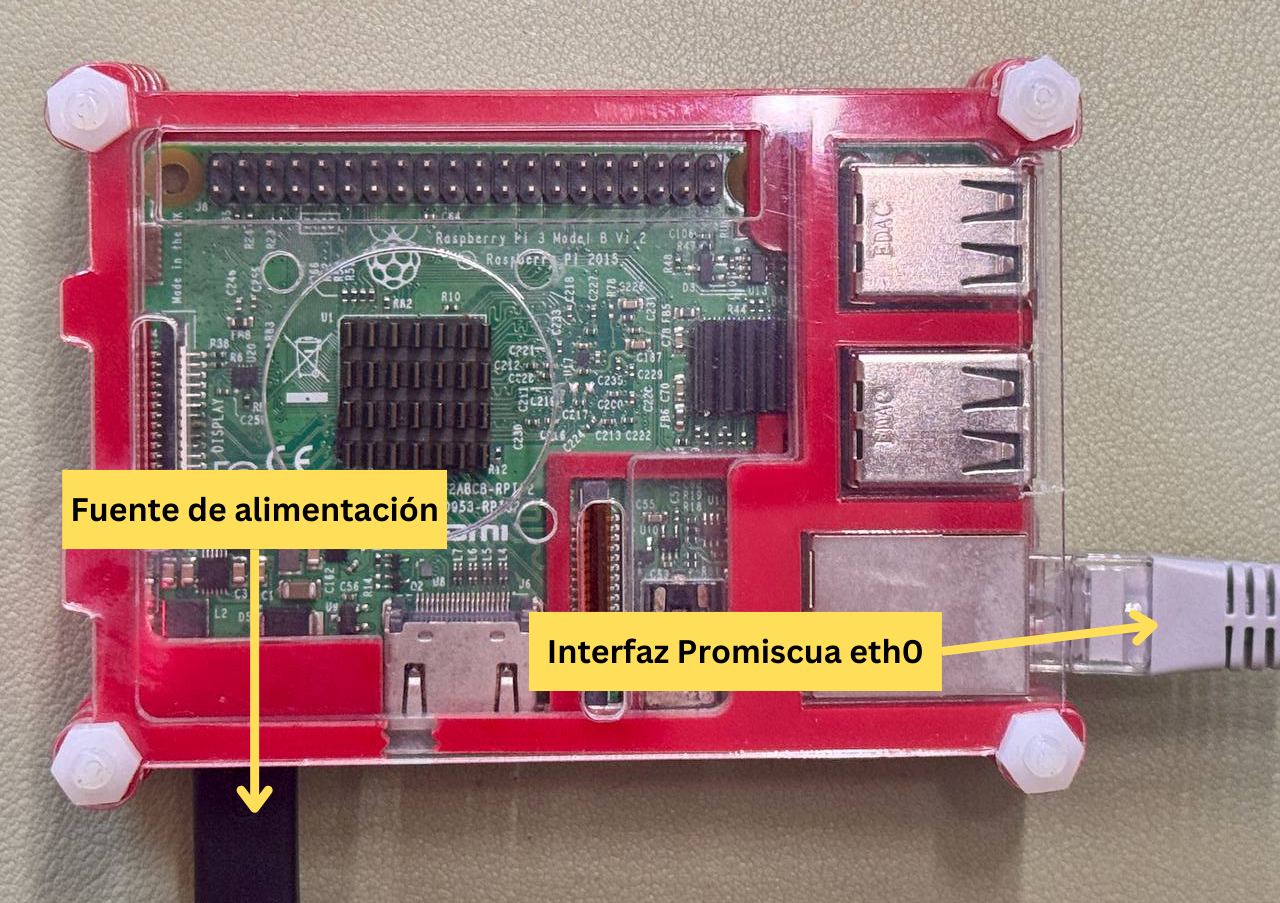
\includegraphics[width=0.7\textwidth]{install/0.3.png}
	\caption{Raspberry Pi 3 actuando como agente.}
	\label{fig:conexion-agente-rpi3}
\end{figure}


\subsubsection{Conexión del switch de la subred secundaria}

En la subred secundaria, el tráfico de red es gestionado por un segundo switch gestionable. Este switch recibe conexión directa al router para proporcionar acceso a internet a los dispositivos conectados.\newline

La \textbf{Raspberry Pi 3 Model B}, que actúa como agente Snort, está conectada al puerto configurado para port mirroring. Su interfaz \texttt{eth0}, operando en modo promiscuo, captura todo el tráfico generado por los dispositivos de la red que están conectados al resto de puertos del switch.\newline

Esta arquitectura permite extender la monitorización a múltiples subredes, manteniendo una estructura modular y escalable dentro del sistema R-Snort.

\begin{figure}[H]
	\centering
	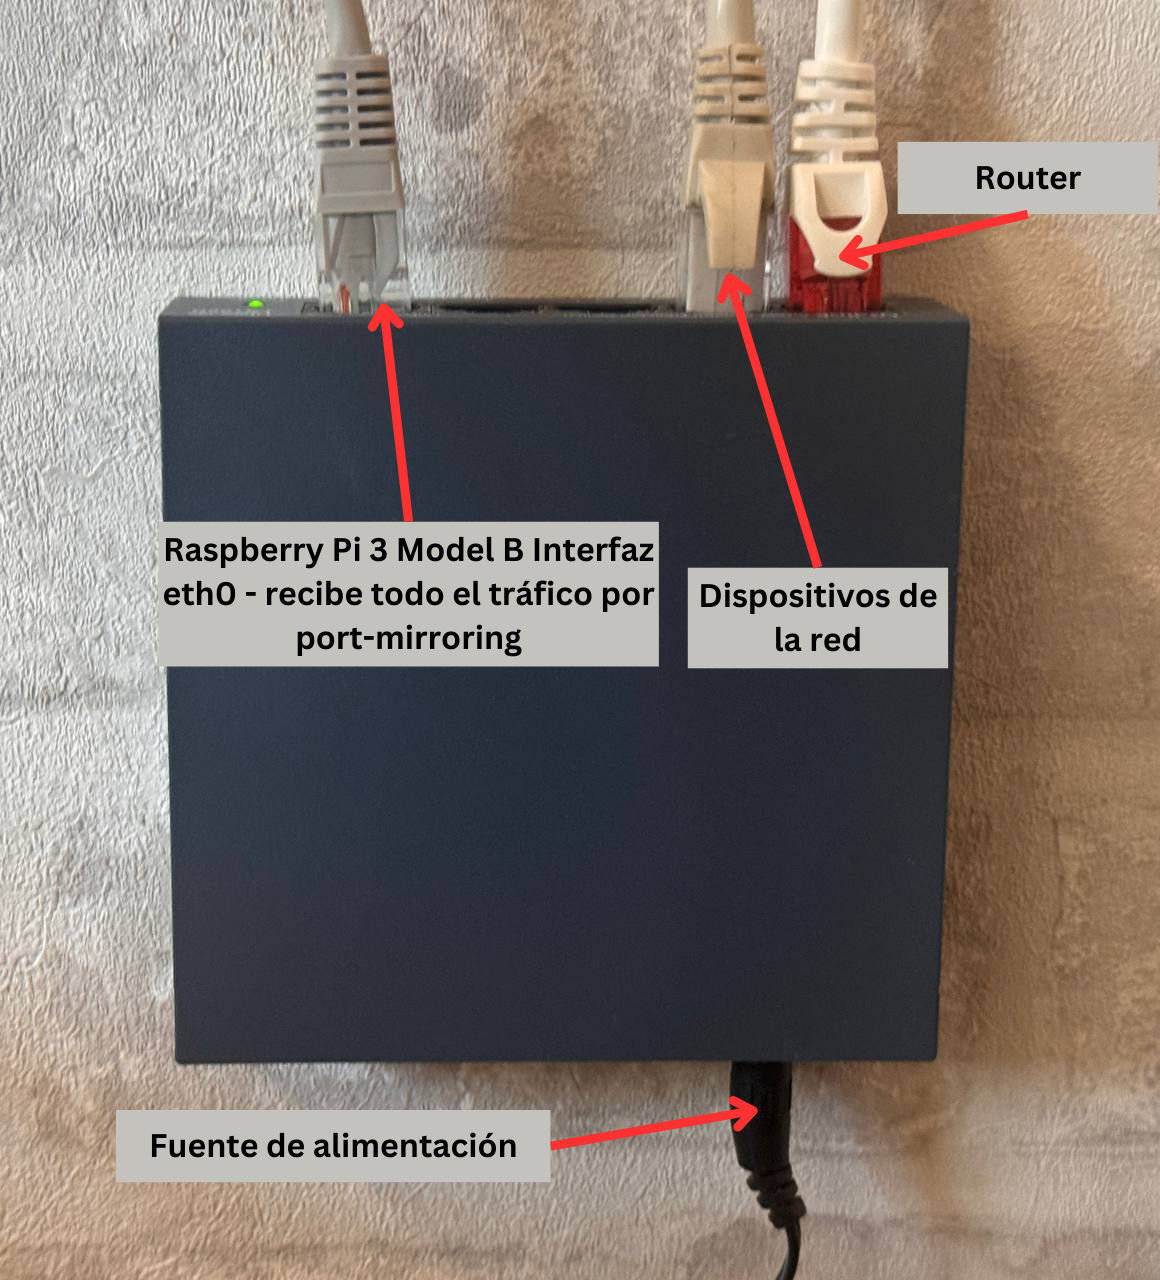
\includegraphics[width=0.5\textwidth]{install/0.4.png}
	\caption{Conexiones del switch secundario.}
	\label{fig:switch-subred2}
\end{figure}


\subsubsection{Instalación de Snort 3 personalizado}

Para completar la preparación del sistema, es necesario instalar Snort versión 3 en ambas Raspberry Pi. Tal como se ha comentado previamente, se utilizará la instancia personalizada desarrollada como complemento de este Trabajo Fin de Grado, optimizada para entornos SOHO y compatible con arquitecturas ARM.\newline

Esta versión incluye todas las dependencias necesarias, configuraciones de rendimiento ajustadas y soporte para bibliotecas como \texttt{Hyperscan}, eliminando la necesidad de instalación manual o intervención compleja por parte del usuario.\newline

El proceso de instalación es completamente automático. Basta con clonar el repositorio correspondiente y ejecutar el script principal:

\newpage

\begin{lstlisting}[language=bash, caption={Instalación de R-Snort personalizada}, label={lst:instalacion-rsnort}]
	git clone https://github.com/deianp189/r-snort-installer.git
	cd r-snort-installer
	sudo ./install_rsnort.sh
\end{lstlisting}

\begin{figure}[H]
	\centering
	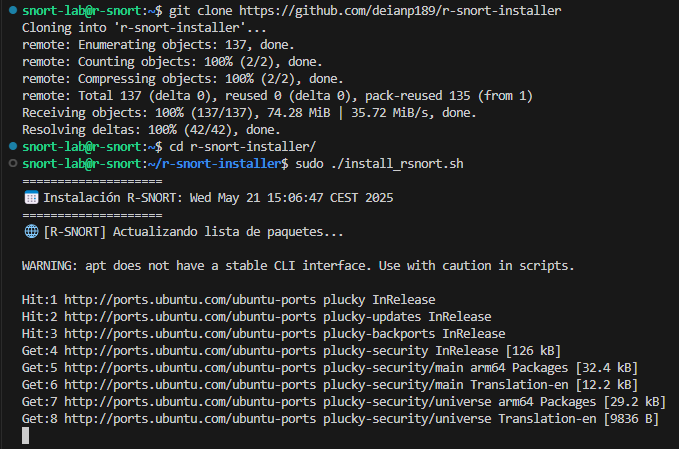
\includegraphics[width=0.7\textwidth]{install/2.png}
	\caption{Inicio de la instalación del agente.}
	\label{fig:inicio-instalacion-rsnort}
\end{figure}

Tras unos 15 minutos en la Raspberry Pi 5, el sistema tendrá Snort 3 instalado, configurado y activo sobre la interfaz elegida por el usuario. Al finalizar, el script ofrece un resumen detallado del estado del sistema, incluyendo información sobre recursos, antivirus y adaptadores de red.

\begin{figure}[H]
	\centering
	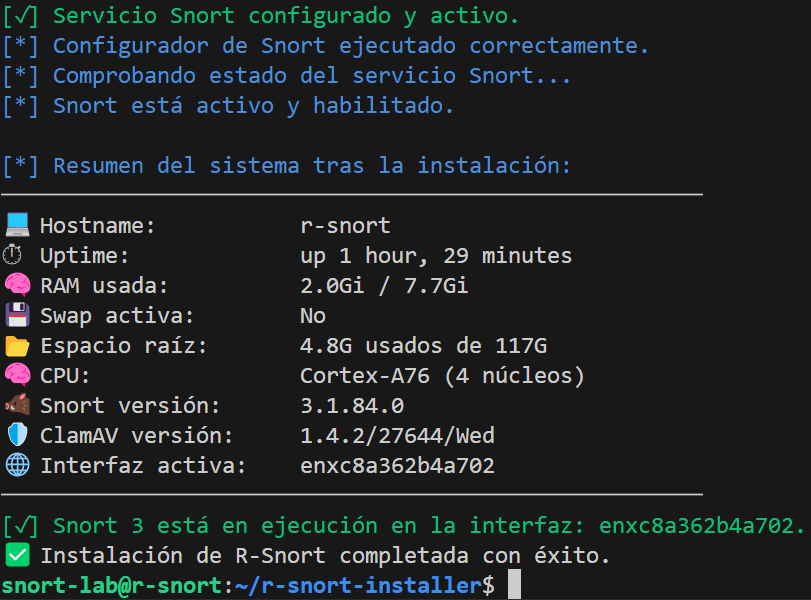
\includegraphics[width=0.7\textwidth]{install/3.png}
	\caption{Resumen tras la instalación.}
	\label{fig:resumen-instalacion-rsnort}
\end{figure}


\subsection{Instalación del agente R-Snort}

La instalación del agente R-Snort se realiza mediante un script completamente automatizado que integra y configura todos los componentes necesarios. Aunque previamente se ha detallado cómo se transforma Snort versión 3 en un sistema funcional mediante el complemento del TFG, este instalador encapsula todo el proceso en una ejecución sencilla y eficiente.\newline

El script realiza las siguientes tareas de forma automática:

\begin{itemize}
	\item Configura Snort 3 para almacenar sus alertas en un archivo específico.
	\item Lanza los servicios de ingestión y métrica que recogen estas alertas y las insertan en una base de datos MariaDB.
	\item Despliega una API REST basada en FastAPI, que permite al módulo central acceder a las alertas y métricas del agente.
	\item Instala y configura Grafana 12, incluyendo un dashboard personalizado que se importa automáticamente.
	\item Registra todos los servicios con systemd para que arranquen de forma persistente.
\end{itemize}

Una vez instalado, el usuario no necesita realizar configuraciones adicionales. El propio sistema indica al final de la instalación las URLs desde las que se puede acceder a la API REST y al panel de Grafana.\newline

El proceso comienza con los siguientes comandos:

\begin{lstlisting}[language=bash, caption={Comandos de instalación del agente}, label={lst:instalacion-snort-agent}]
	git clone https://github.com/deianp189/snort-agent.git
	cd snort-agent
	sudo ./install.sh
\end{lstlisting}

\begin{figure}[H]
	\centering
	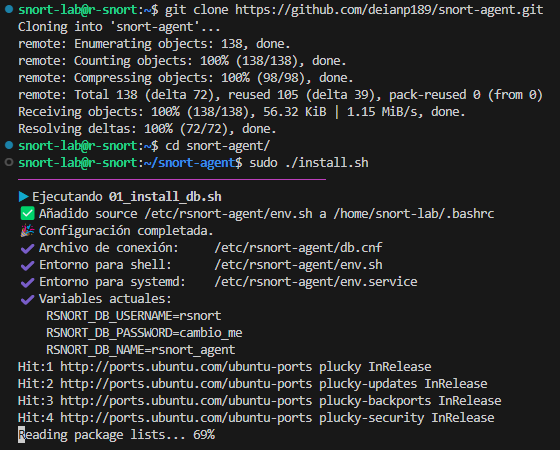
\includegraphics[width=0.6\textwidth]{install/4.png}
	\caption{Inicio de la instalación del agente.}
	\label{fig:inicio-snort-agent}
\end{figure}

La duración estimada es de entre 5 y 8 minutos, dependiendo de la conexión a internet. El usuario simplemente debe esperar mientras el sistema realiza toda la configuración necesaria.

\begin{figure}[H]
	\centering
	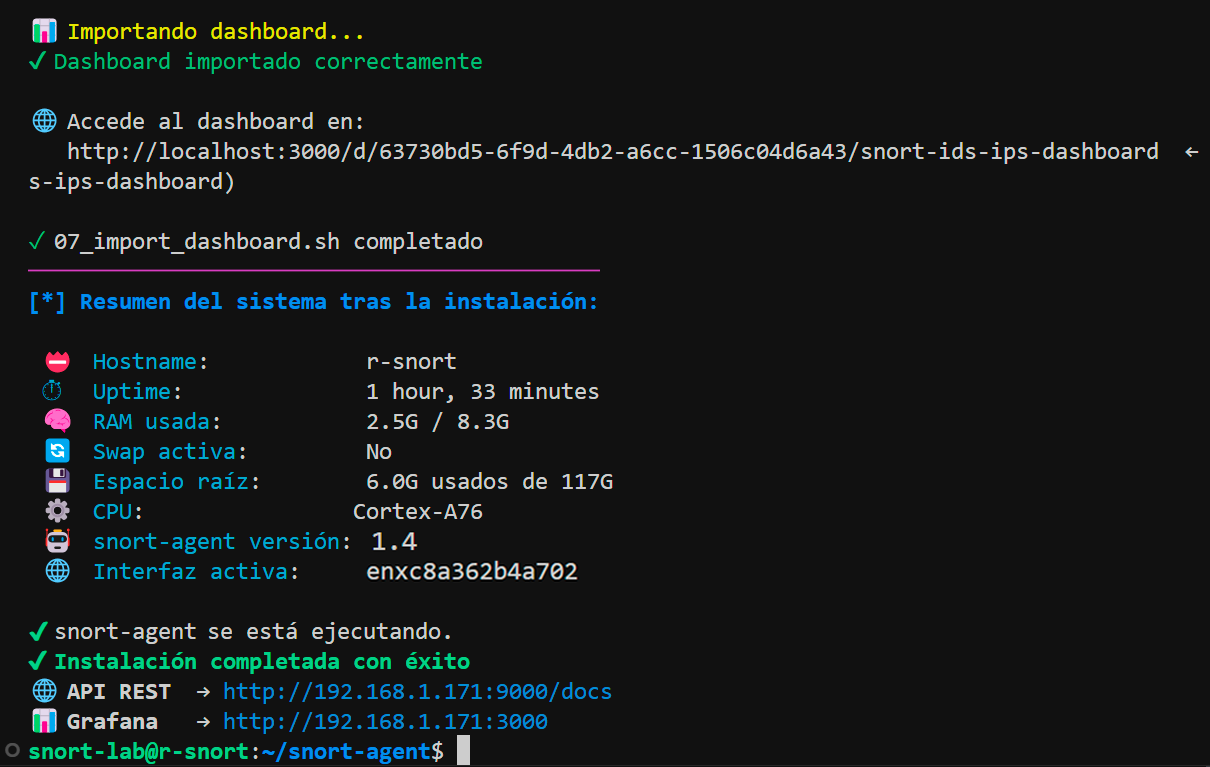
\includegraphics[width=0.7\textwidth]{install/5.png}
	\caption{Finalización y resumen del agente instalado.}
	\label{fig:resumen-snort-agent}
\end{figure}


\subsection{Instalación del módulo central de R-Snort}

Una vez instalado el agente, puede transformarse en el \textbf{módulo central de R-Snort} ejecutando un segundo instalador. Este script despliega el sistema completo de gestión: compila el frontend desarrollado en Angular, lo integra dentro del backend en Spring Boot y lo configura como servicio persistente mediante \texttt{systemd}, asegurando su ejecución tras cada reinicio del sistema.

\begin{lstlisting}[language=bash, caption={Comandos de instalación del agente}, label={lst:instalacion-snort-agent}]
	git clone https://github.com/deianp189/r-snort-central-module-installer.git
	cd r-snort-central-module-installer/scripts
	sudo ./run_all
\end{lstlisting}

\begin{figure}[H]
	\centering
	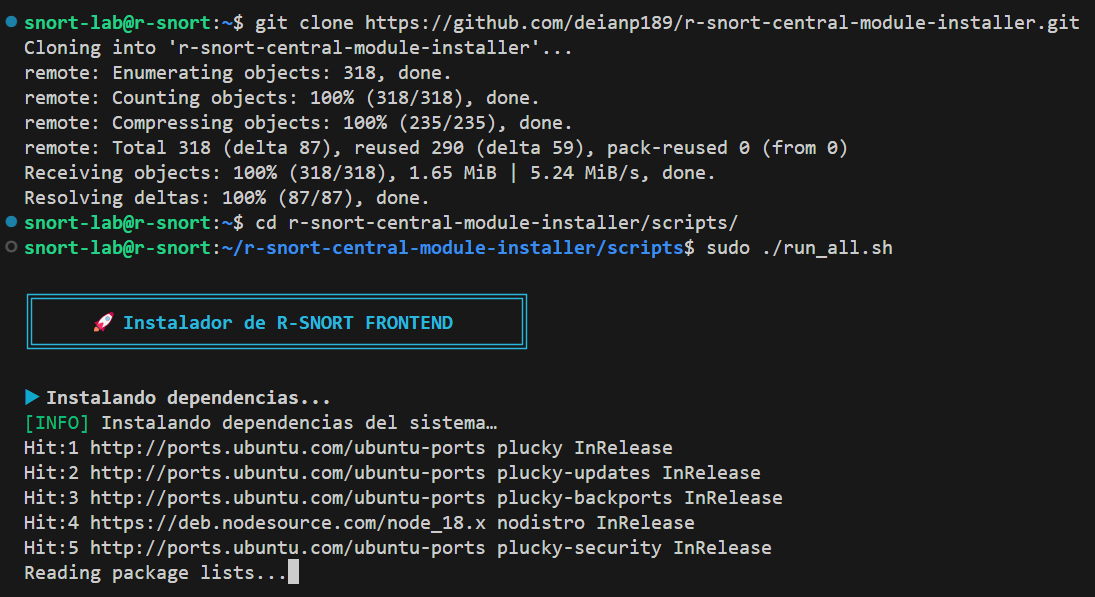
\includegraphics[width=0.8\textwidth]{install/6.png}
	\caption{Inicio de la instalación del módulo central.}
	\label{fig:inicio-central-module}
\end{figure}

\newpage

Durante la instalación, el usuario solo debe indicar sus credenciales de administrador y decidir si desea declarar más agentes manualmente. En este caso se optó por omitir esa configuración, ya que la interfaz web permite añadirlos posteriormente, lo cual resulta más cómodo y sirve para demostrar la funcionalidad del sistema.\newline

El proceso dura aproximadamente cinco minutos y finaliza mostrando un resumen detallado del entorno, así como la dirección web desde la cual puede accederse al panel de administración.

\begin{figure}[H]
	\centering
	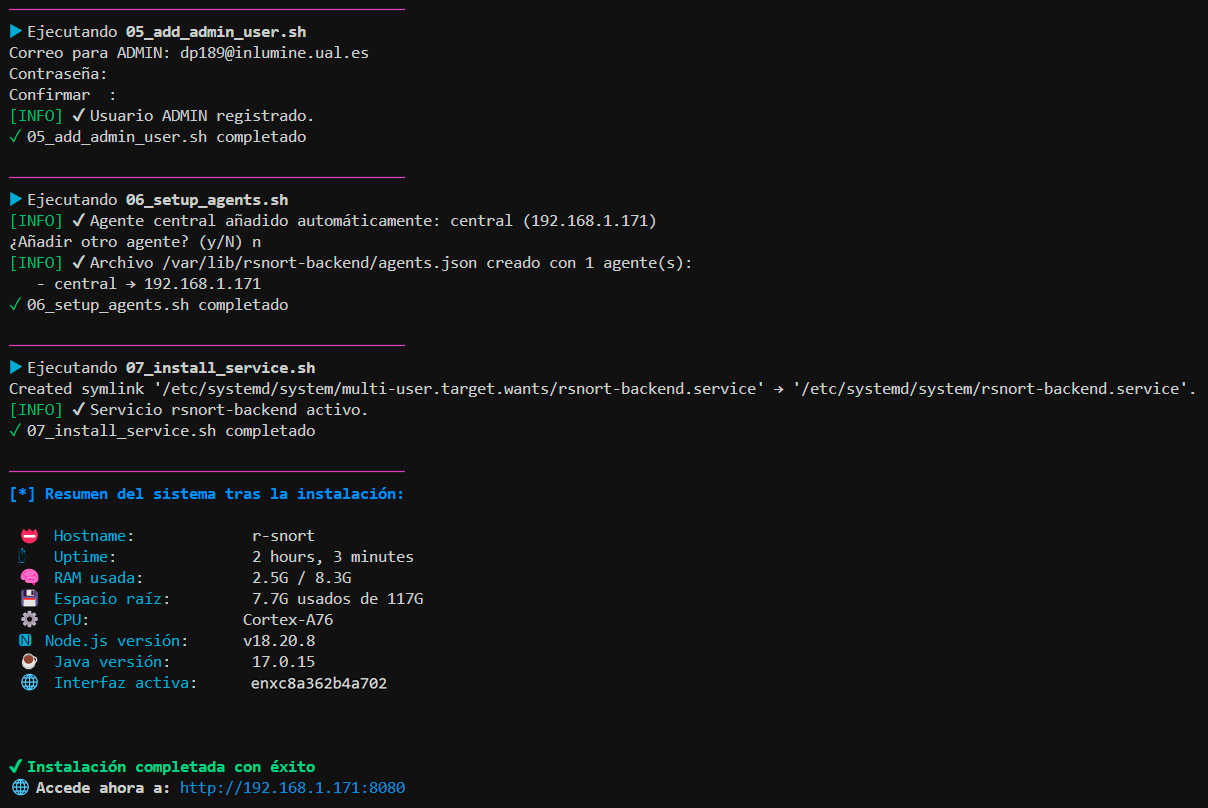
\includegraphics[width=0.9\textwidth]{install/7.png}
	\caption{Finalización y resumen del módulo central.}
	\label{fig:fin-central-module}
\end{figure}

\newpage


\section{Utilización y pruebas}

\subsection{Configuración}

Tras completar el proceso de instalación, el acceso a la interfaz web de R-Snort se realiza fácilmente introduciendo en el navegador la dirección \texttt{http://<IP-del-módulo-central>:8080} (También se muestra con exactitud al finalizar la instalación). La autenticación se efectúa mediante las credenciales proporcionadas por el usuario durante la instalación del módulo central.

\begin{figure}[H]
	\centering
	\includegraphics[width=0.8\textwidth]{configuracion/1.png}
	\caption{Pantalla de inicio de sesión del sistema R-Snort.}
	\label{fig:login-rsnort}
\end{figure}

Una vez autenticado, se accede a la pestaña \textbf{Overview}, que presenta un panel general con gráficas dinámicas alimentadas por Grafana. Estas gráficas se generan a partir de los datos almacenados en MariaDB y reflejan información escogida con sumo cuidado como: número de alertas por severidad (alta, media y baja), protocolos implicados, tipos de alertas más frecuentes, y direcciones IP origen. Todo ello permite una visualización rápida y efectiva del estado de la red.

\begin{figure}[H]
	\centering
	\includegraphics[width=0.8\textwidth]{configuracion/2.png}
	\caption{Panel general con métricas y alertas.}
	\label{fig:overview-rsnort}
\end{figure}

\newpage

En la pestaña \textbf{Alertas}, el usuario puede inspeccionar de forma detallada las últimas alertas generadas, agrupadas por severidad. Esta vista incluye un panel de resumen y una tabla con todas las alertas clasificadas por fecha, origen, destino y tipo de amenaza detectada. Además, se ofrece la opción de descargar alertas individuales por agente o en su totalidad para un análisis forense posterior.

\begin{figure}[H]
	\centering
	\includegraphics[width=0.9\textwidth]{configuracion/3.png}
	\caption{Panel de alertas clasificadas por severidad.}
	\label{fig:alertas-rsnort}
\end{figure}

La pestaña \textbf{Reglas} muestra todas las reglas actualmente activas del archivo \texttt{custom.rules}, incluyendo aquellas diseñadas para detectar fuga de datos sensibles como correos electrónicos, tarjetas de crédito o números NUSS. El sistema permite añadir nuevas reglas y elimina automáticamente aquellas duplicadas o malformadas, previniendo fallos de carga en Snort.

\begin{figure}[H]
	\centering
	\includegraphics[width=0.9\textwidth]{configuracion/4.png}
	\caption{Gestión de reglas Snort desde la interfaz.}
	\label{fig:reglas-rsnort}
\end{figure}

\newpage

En la pestaña \textbf{Estado}, se presentan datos sobre el uso de recursos del sistema (CPU, disco, temperatura) a lo largo del tiempo, gracias a la integración con Grafana. Además, se muestra el estado actual de Snort, la última alerta capturada y la posibilidad de reiniciar los servicios involucrados (\texttt{snort}, \texttt{ingest}, \texttt{metrics}).

\begin{figure}[H]
	\centering
	\includegraphics[width=0.9\textwidth]{configuracion/5.png}
	\caption{Monitorización de temperatura, CPU y estado del servicio.}
	\label{fig:estado-central}
\end{figure}

Justo debajo, aparecen tarjetas individuales por cada agente declarado. En este caso se muestra el módulo central. Desde aquí se puede reiniciar cada servicio por separado o eliminar el agente (con doble confirmación). Esta vista también permite validar si Snort está en ejecución, cuántas alertas ha generado y cuál fue la última detectada.

\begin{figure}[H]
	\centering
	\includegraphics[width=0.9\textwidth]{configuracion/6.png}
	\caption{Estado detallado del agente central.}
	\label{fig:estado-agente-central}
\end{figure}

\newpage

El menú desplegable de selección de agente permite cambiar rápidamente de instancia monitorizada. Inicialmente solo está presente el módulo central, pero se pueden añadir más agentes en caliente.

\begin{figure}[H]
	\centering
	\includegraphics[width=0.9\textwidth]{configuracion/7.png}
	\caption{Menú de selección de agentes activos.}
	\label{fig:selector-agentes}
\end{figure}

Para registrar un nuevo agente, basta con pulsar el botón \texttt{+} de la esquina superior derecha. Se abrirá un formulario donde se especifica el nombre del agente y su dirección IP. El sistema previene duplicados automáticamente.

\begin{figure}[H]
	\centering
	\includegraphics[width=0.7\textwidth]{configuracion/8.png}
	\caption{Formulario para añadir un nuevo agente Snort.}
	\label{fig:agregar-agente}
\end{figure}

Una vez añadido, el nuevo agente aparecerá en el desplegable y el dashboard se actualizará dinámicamente con sus métricas y alertas. En el ejemplo mostrado, se ha conectado un segundo agente en la subred 2, el cual genera menos tráfico por haber estado inactivo durante parte del día.

\begin{figure}[H]
	\centering
	\includegraphics[width=0.7\textwidth]{configuracion/9.png}
	\caption{Visualización de métricas del agente secundario.}
	\label{fig:dashboard-agente-secundario}
\end{figure}

\newpage

Finalmente, en la vista de \textbf{Estado} ahora se muestran múltiples tarjetas, una por cada agente activo. Cada una de ellas permite gestionar de forma independiente los servicios del agente y consultar su última alerta. Además, se incluye la opción de eliminar el agente de forma segura mediante una doble confirmación visual.

\begin{figure}[H]
	\centering
	\includegraphics[width=0.9\textwidth]{configuracion/10.png}
	\caption{Gestión avanzada de agentes Snort desde la interfaz.}
	\label{fig:estado-multiple-agentes}
\end{figure}

\subsection{Pruebas de rendimiento}

Gracias a que el propio diseño del módulo central de de R-Snort cuenta con métricas del sistema que se actualizan en tiempo real vamos a aprovechar estas con el fin de hacer unas pruebas de rendimiento bajo uso normal o moderado del sistema, es decir simplemente escuchando la red sin ningún tipo de ataque ni alteración que pueda disparar las alertas y posteriormente haremos un envio de datos masivos para tratar de comprobar la estabilidad del sistema y como responde ante dicho envio de datos.

\subsubsection{Monitorización del rendimiento en funcionamiento normal}

Para analizar el comportamiento del sistema R-Snort durante su funcionamiento ordinario, se ha optado por utilizar directamente los paneles de Grafana integrados en la interfaz web del módulo central. Esta decisión no solo permite evitar herramientas externas, sino que además ilustra la capacidad del propio sistema para autodiagnosticarse en tiempo real, un aspecto clave en entornos de monitorización profesional.

Las métricas analizadas han sido las siguientes:

\begin{itemize}
	\item \textbf{Temperatura de la CPU}: Como se aprecia en la Figura~\ref{fig:temp-normal}, la temperatura del sistema se mantiene entre los 46 y 51 grados durante un intervalo prolongado de uso normal. Estas cifras se encuentran dentro de los márgenes aceptables para una Raspberry Pi 5 en carga moderada, lo cual indica una refrigeración adecuada y ausencia de sobrecalentamientos.
	
	\item \textbf{Uso de CPU (\%)}: Tal como muestra la Figura~\ref{fig:cpu-normal}, el consumo de CPU se mantiene mayoritariamente por debajo del 10\%, con algunos picos aislados que no superan el 30\%. Este comportamiento es coherente con un sistema que opera de manera eficiente, sin procesos en bucle ni sobrecargas injustificadas.
	
	\item \textbf{Uso de disco}: También representado en la Figura~\ref{fig:cpu-normal}, el uso del disco se estabiliza en torno al 7\% de capacidad total. Esta métrica sugiere que los logs y la base de datos de alertas no saturan el almacenamiento durante la operación diaria del sistema.
\end{itemize}

\begin{figure}[H]
	\centering
	\includegraphics[width=0.95\textwidth]{benchmark/1.png}
	\caption{Temperatura de la CPU durante funcionamiento normal.}
	\label{fig:temp-normal}
\end{figure}

\begin{figure}[H]
	\centering
	\includegraphics[width=0.95\textwidth]{benchmark/2.png}
	\caption{Consumo de CPU y uso de disco durante funcionamiento normal.}
	\label{fig:cpu-normal}
\end{figure}

En conjunto, estos resultados permiten afirmar que R-Snort presenta un comportamiento estable y eficiente en condiciones de uso normales. Las gráficas no solo validan la correcta instalación de los scripts, sino también la eficacia de los servicios en ejecución, sin que se produzcan cuellos de botella ni compromisos en la estabilidad del sistema.

\subsubsection{Análisis de rendimiento en situación de estrés}

Para evaluar el comportamiento del sistema R-Snort ante un escenario de uso intensivo, se ha llevado a cabo una prueba de estrés basada en el envío masivo de paquetes desde varias terminales empleando \texttt{iperf3} contra la interfaz promiscua del agente central. Esta situación simula un ataque de denegación de servicio distribuido (DDoS), en el cual se pretende saturar tanto la red como los recursos del sistema, y evaluar la capacidad de detección y resistencia de la Raspberry Pi 5 actuando como nodo central.

\subsubsection*{Descripción del experimento}
Durante el experimento se han abierto múltiples instancias concurrentes de \texttt{iperf3}, generando tráfico simultáneo a través de diferentes puertos. A su vez, se ha mantenido Snort 3 activo con sus correspondientes preprocesadores y reglas personalizadas, recogiendo y analizando cada paquete de red. Las métricas de rendimiento se han recogido mediante Grafana, obteniendo series temporales de las siguientes variables clave:

\begin{itemize}
	\item Uso de CPU (\%).
	\item Uso de disco (\%).
	\item Temperatura de la CPU (ºC).
	\item Alertas registradas por severidad y tipo.
\end{itemize}

\subsubsection*{Resultados observados}

\begin{itemize}
	\item En la Figura \ref{fig:bench-alertas-normales}, correspondiente al tráfico normal previo al ataque, se observa un número moderado de alertas, con predominancia de alertas de severidad baja o media, originadas principalmente por tráfico ICMP o DNS.
	
	\item En la Figura \ref{fig:bench-uso-cpu-disco}, tras iniciar la prueba de carga, se detecta un incremento inmediato y sostenido del uso de CPU, alcanzando picos superiores al 60\% de uso. Sin embargo, el uso de disco permanece estable, gracias al sistema de rotación de logs y al diseño eficiente del almacenamiento.
	
	\item La Figura \ref{fig:bench-temp-cpu} muestra el incremento progresivo de la temperatura del sistema, alcanzando máximos en torno a los 62 grados (con refrigeración) durante la fase más intensa del ataque. A pesar del aumento térmico, el sistema mantuvo la estabilidad operativa sin pérdidas de servicio.
	
\end{itemize}

\subsubsection*{Conclusiones}
Estas pruebas demuestran que el sistema R-Snort es capaz de soportar picos de carga elevados durante periodos prolongados sin comprometer la integridad de la plataforma. El uso sostenido de CPU y el aumento térmico son respuestas esperadas bajo estas condiciones, pero en ningún momento se observaron reinicios, errores del servicio o pérdida de conectividad. Este comportamiento refuerza la validez del diseño implementado para entornos SOHO donde la seguridad, la fiabilidad y la eficiencia energética son prioritarias.

\begin{figure}[H]
	\centering
	\includegraphics[width=\textwidth]{benchmark/3.png}
	\caption{Alertas registradas durante tráfico normal.}
	\label{fig:bench-alertas-normales}
\end{figure}

\begin{figure}[H]
	\centering
	\includegraphics[width=\textwidth]{benchmark/5.png}
	\caption{Porcentaje de uso de CPU y disco durante el ataque.}
	\label{fig:bench-uso-cpu-disco}
\end{figure}

\begin{figure}[H]
	\centering
	\includegraphics[width=\textwidth]{benchmark/4.png}
	\caption{Temperatura de la CPU durante la fase de estrés.}
	\label{fig:bench-temp-cpu}
\end{figure}

Para este ataque masivo con el objetivo de someter al sistema R-Snort a condiciones extremas y evaluar su capacidad de detección y estabilidad bajo situaciones de estrés, se diseñó un script que ejecuta múltiples ataques en paralelo. Este script fue lanzado desde una máquina externa WSL y permitió generar un volumen de tráfico malicioso elevado, simulando un escenario realista de intrusión.\newline

Las pruebas se ha realizado activando simultáneamente diferentes vectores de ataque: un \textit{TCP SYN Flood}, un \textit{ICMP Flood}, un escaneo agresivo con \textit{nmap}, tráfico constante con \textit{iperf3}, y un intento limitado de fuerza bruta sobre el servicio \texttt{ssh} utilizando \textit{hydra}. Cada ejecución del script puede adaptarse para utilizar diferentes puertos de iperf, lo que permite lanzarlo desde varias terminales en paralelo sin conflictos.\newline

El siguiente fragmento muestra el contenido del script utilizado:

\begin{lstlisting}[language=bash,caption={Script para generar ataques masivos contra R-Snort},label={lst:ataques-masivos}]
	# PUERTO UNICO POR INSTANCIA
	PUERTO_IPERF="${1:-5201}"
	
	echo "[+] ATAQUE desde terminal con IPERF en puerto $PUERTO_IPERF"
	echo "==============================================="
	
	# 1. TCP SYN Flood
	echo "[1] Iniciando TCP SYN Flood con hping3..."
	sudo hping3 -S --flood -p 80 $R_SNORT_IP &
	
	# 2. ICMP Flood
	echo "[2] Iniciando ICMP Flood..."
	sudo hping3 -1 --flood $R_SNORT_IP &
	
	# 3. Escaneo nmap agresivo
	echo "[3] Lanzando escaneo Nmap agresivo..."
	sudo nmap -sS -sU -T4 -A $R_SNORT_IP --reason --script "default" -p- &
	
	# 4. Tráfico continuo con iperf3 (en puerto variable)
	echo "[4] Ejecutando iperf3 -c $R_SNORT_IP -p $PUERTO_IPERF ..."
	iperf3 -c $R_SNORT_IP -p $PUERTO_IPERF -t 60 -b 100M &
	
	# 5. Ataque de fuerza bruta con hydra (limitado)
	echo "[5] Simulando fuerza bruta con Hydra..."
	hydra -l admin -p admin ssh://$R_SNORT_IP -t 4 -V -f &
	
	echo "==============================================="
	echo "Todos los ataques están en ejecución. Observar las gráficas."
\end{lstlisting}

Este enfoque permitió verificar no solo la capacidad del sistema para generar alertas ante ataques múltiples, sino también analizar el rendimiento de la Raspberry Pi bajo carga, así como la eficacia del almacenamiento de alertas y la visualización en tiempo real mediante Grafana.

\newpage

\subsection{Pruebas funcionales}

Para el apartado de pruebas se pretende verificar la estabilidad y eficiencia de la interfaz frontend de R-Snort ante un volumen extremo de alertas generado durante las pruebas de estrés con tráfico malicioso y las demás funcionalidades del ecosistema R-Snort.\newline

\subsubsection{Registro de alertas masivas}

Durante los benchmarks realizados en el apartado \textit{3.3.2 Benchmark de rendimiento}, se generaron decenas de miles de alertas mediante ataques simulados que incluían DDoS, escaneos agresivos y envíos masivos de paquetes ICMP, TCP y UDP con herramientas como \texttt{hping3}, \texttt{iperf3} y \texttt{nmap}. Como resultado, Snort detectó y registró más de \textbf{250.000 alertas} en un intervalo de pocas horas.\newline

La interfaz de R-Snort, tanto en la vista de alertas como en el panel de Grafana incrustado, fue puesta a prueba visualizando este gran volumen de información. Se evaluaron los tiempos de carga, la fluidez al cambiar entre vistas y la capacidad de la base de datos para manejar consultas masivas sin cuellos de botella visibles.\newline

\textbf{Resultado:}  
A pesar del gran volumen de datos, la aplicación web se comportó de forma fluida y sin fallos. En la vista \texttt{Alertas}, se mostraron correctamente los conteos por severidad, así como las tablas paginadas con miles de resultados. Por otro lado, los dashboards de Grafana embebidos en la sección \texttt{Overview} actualizaron en tiempo real los gráficos de tendencias por severidad, tipos de alerta, IPs de origen y protocolos.\newline

Este comportamiento confirma que R-Snort es capaz de operar eficazmente incluso en escenarios de saturación de red, cumpliendo así uno de sus objetivos clave como herramienta profesional para entornos empresariales.

\textbf{Componentes implicados:}
\begin{itemize}
	\item Backend de ingestión de alertas (\texttt{ingest\_service.py})
	\item API REST del agente y del módulo central
	\item Base de datos MariaDB para almacenamiento de alertas
	\item Frontend Angular (tablas, visualización por severidad)
	\item Dashboards de Grafana incrustados (Overview)
\end{itemize}

\begin{figure}[H]
	\centering
	\includegraphics[width=0.8\textwidth]{pruebas/1.png}
	\caption{Dashboard de Grafana mostrando más de 250.000 alertas tras una prueba de estrés. Se observan tendencias por severidad, protocolo e IPs de origen.}
	\label{fig:alertas_masivas_grafana}
\end{figure}

\begin{figure}[H]
	\centering
	\includegraphics[width=0.8\textwidth]{pruebas/2.png}
	\caption{Panel de alertas en la aplicación web con visualización correcta de alertas severas, medias y bajas tras las pruebas de carga.}
	\label{fig:alertas_masivas_webapp}
\end{figure}

\subsubsection{Recorrido de las funciones}
\label{sec:funcionamiento}

En esta sección se describen algunas de las funcionalidades adicionales del sistema R-Snort implementadas en la interfaz web, que no habían sido abordadas o lo fueron muy superficialmente en apartados anteriores. Estas funcionalidades están orientadas a facilitar el uso y mantenimiento del sistema por parte de un administrador de red, permitiendo gestionar reglas, supervisar el estado de los agentes, y acceder a los registros generados por Snort.

\paragraph{Descarga de logs archivados}

Una de las funcionalidades destacadas es el sistema de rotación y archivado de logs implementado en los agentes. Este sistema previene que los archivos de alertas crezcan indefinidamente, lo cual es especialmente útil en entornos con tráfico elevado. Los archivos rotados se comprimen automáticamente y se almacenan como copias de respaldo, accesibles desde la interfaz. Se ha incorporado un botón para descargar estos logs archivados, lo cual resulta especialmente útil para tareas de análisis forense o revisión posterior.

\begin{figure}[H]
	\centering
	\includegraphics[width=0.5\textwidth]{pruebas/3.png}
	\caption{Descarga de archivos de logs archivados generados por el sistema de rotación.}
	\label{fig:descarga_logs_archivados}
\end{figure}

\paragraph{Exportación de alertas activas en CSV}

Además de los logs comprimidos, el sistema permite exportar las alertas activas en formato \texttt{.csv}, tanto para un agente específico como para todos los agentes de la red. Esta funcionalidad permite al administrador exportar la información y analizarla con herramientas externas como hojas de cálculo o entornos de análisis de datos.

\begin{figure}[H]
	\centering
	\includegraphics[width=0.8\textwidth]{pruebas/4.png}
	\caption{Opciones de descarga de alertas activas por agente o globales en formato CSV.}
	\label{fig:descarga_alertas_csv}
\end{figure}

\paragraph{Añadir reglas personalizadas a Snort}

En el módulo de gestión de reglas, el sistema permite añadir nuevas reglas personalizadas al archivo \texttt{custom.rules} del agente. El formulario de inserción verifica automáticamente que la regla no esté duplicada y que su sintaxis sea válida. En caso de error, se notifica al usuario de forma clara. A continuación, se muestra la creación de una nueva regla para detectar intentos de acceso externo al puerto 22 (SSH).

\begin{figure}[H]
	\centering
	\includegraphics[width=0.8\textwidth]{pruebas/5.png}
	\caption{Inserción de una nueva regla de detección de conexiones SSH no autorizadas.}
	\label{fig:insertar_regla_ssh}
\end{figure}

Una vez agregada, la regla aparece listada junto a las demás reglas activas. Esto permite al administrador confirmar su incorporación y tener una visión clara de las políticas de detección vigentes en el sistema.

\begin{figure}[H]
	\centering
	\includegraphics[width=0.8\textwidth]{pruebas/6.png}
	\caption{Regla personalizada añadida correctamente al sistema del agente central.}
	\label{fig:regla_ssh_insertada}
\end{figure}

\paragraph{Eliminación segura de reglas}

Del mismo modo, el sistema permite eliminar reglas personalizadas de forma controlada. Cada eliminación requiere confirmación explícita por parte del usuario para evitar modificaciones accidentales.

\begin{figure}[H]
	\centering
	\includegraphics[width=0.5\textwidth]{pruebas/7.png}
	\caption{Confirmación de eliminación de una regla personalizada.}
	\label{fig:eliminar_regla}
\end{figure}

\paragraph{Gestión de agentes y eliminación con verificación}

En cuanto a la gestión de agentes, el sistema permite también eliminar instancias previamente registradas. Dado que esta acción puede afectar la supervisión de una subred completa, el sistema solicita una doble confirmación, reforzando así la seguridad en las operaciones críticas.

\begin{figure}[H]
	\centering
	\includegraphics[width=0.8\textwidth]{pruebas/8.png}
	\caption{Verificación antes de eliminar un agente de la interfaz.}
	\label{fig:eliminar_agente}
\end{figure}

\paragraph{Supervisión de servicios y reinicio desde la interfaz}

Por último, el panel de estado permite visualizar en tiempo real la disponibilidad de los servicios principales de cada agente (Snort, ingestión de alertas y métricas del sistema). En caso de que algún servicio se encuentre caído o inactivo, el administrador puede reiniciarlo directamente desde la interfaz sin necesidad de acceso por terminal. Esto proporciona una herramienta de recuperación rápida ante fallos.

\begin{figure}[H]
	\centering
	\includegraphics[width=0.8\textwidth]{pruebas/9.png}
	\caption{Estado de los servicios de los agentes y opción de reinicio remoto.}
	\label{fig:estado_servicios_agentes}
\end{figure}

Estas pruebas funcionales demuestran que el sistema R-Snort no solo es capaz de detectar tráfico sospechoso y generar alertas, sino que también proporciona un conjunto de herramientas completas para la administración y supervisión de agentes, reglas y registros, mejorando la capacidad operativa y reduciendo la necesidad de intervención manual.

\section{Resumen}

El capítulo muestra un caso práctico exitoso del sistema R-Snort implementado en un entorno realista para pequeñas oficinas (SOHO). Se ha utilizado una infraestructura sencilla pero al mismo tiempo viable, formada por un módulo central basado en Raspberry Pi 5 y un agente secundario en Raspberry Pi 3, ambos conectados a switches gestionables que facilitan la monitorización eficiente del tráfico mediante port mirroring.\newline

El módulo central integra de manera el backend en Spring Boot, la interfaz web desarrollada en Angular, la base de datos MariaDB y el dashboard interactivo en Grafana, proporcionando una solución completa de gestión centralizada. Por su parte, el ambos agentes ejecutan una versión optimizada de Snort 3 (desarrollada en el Complemento del TFG), adaptada específicamente para dispositivos de bajo consumo.\newline

La instalación se destaca por ser completamente automatizada gracias a scripts especializados, lo que simplifica considerablemente la implementación en entornos reales. Las pruebas efectuadas han demostrado de manera concluyente que R-Snort maneja sin problemas grandes volúmenes de alertas (superiores a 250.000), manteniendo un rendimiento estable y una visualización fluida y dinámica de la información crítica.\newline

Finalmente, las pruebas funcionales adicionales han confirmado la eficacia y fiabilidad del sistema, destacando funcionalidades imporantantes en el ámbito de la ciberseguridad y la administración de sistemas como la rotación y archivado automático de logs, la exportación sencilla de alertas, la gestión dinámica de reglas personalizadas y la administración remota intuitiva de servicios. Todo ello refuerza claramente el valor práctico del proyecto R-Snort como herramienta profesional, accesible y eficaz para la seguridad y supervisión de redes empresariales pequeñas y medianas.






\clearpage
\null
\thispagestyle{empty}
\newpage
\chapter{Resultados y discusión}

\section{Resultados obtenidos}

El sistema R-Snort, tras su despliegue en un entorno simulado de red tipo SOHO y bajo condiciones de uso realista, ha permitido explorar y validar de forma práctica tanto la viabilidad técnica del ecosistema como su utilidad operativa para pequeñas y medianas empresas. A continuación se presentan los resultados obtenidos durante la fase experimental, diferenciando entre los aspectos de funcionalidad, rendimiento, experiencia de usuario y capacidad de adaptación.

\subsection{Eficacia en la detección de amenazas}

Durante la batería de pruebas funcionales, el sistema fue capaz de identificar un amplio rango de incidentes de seguridad: desde escaneos básicos de puertos y ataques ICMP, hasta patrones de exfiltración de datos y tráfico anómalo en protocolos DNS y SNMP. Las alertas generadas por Snort 3 fueron correctamente recogidas por el backend, almacenadas en la base de datos y presentadas en tiempo real a través del frontend (véase Figuras \ref{fig:overview-rsnort} y \ref{fig:alertas-rsnort}). Cabe destacar que la integración con Grafana permitió visualizar tendencias y picos de actividad, lo que facilita la rápida identificación de eventos anómalos o posibles intentos de actividad maliciosa o intrusión además de filtración de datos. Esta capacidad de monitorización continua es importante para el entorno PYME, donde la inmediatez en la detección puede suponer la diferencia entre contener un incidente o sufrir un compromiso mayor.\newline

En las pruebas orientadas a la gestión de reglas, el sistema demostró flexibilidad: fue posible añadir, modificar y eliminar reglas personalizadas desde la interfaz gráfica, reflejándose los cambios en el comportamiento del sensor sin requerir intervención manual en consola. Sin embargo, debe reconocerse que, aunque la interfaz es intuitiva, la comprensión de la lógica subyacente a cada regla aún requiere cierto conocimiento técnico, lo que podría limitar la autonomía del usuario final en escenarios menos formados.

\subsection{Rendimiento y escalabilidad}

En términos de rendimiento, la solución mostró un comportamiento estable ante tráfico normal y bajo cargas elevadas inducidas por ataques simulados (véanse Figuras \ref{fig:temp-normal} a \ref{fig:bench-temp-cpu} y el panel de Grafana 3.29). Durante las pruebas de estrés, la Raspberry Pi 5 mantuvo un uso de CPU y temperatura dentro de márgenes aceptables, sin caídas del servicio ni pérdida de alertas. El almacenamiento de eventos alcanzó volúmenes superiores a 250.000 alertas, gestionadas correctamente gracias al sistema de rotación y archivado automático de logs.\newline

No obstante, se identifican ciertos límites en la capacidad de procesamiento: bajo ataques DDoS prolongados, el retardo en la inserción de nuevas alertas aumentó ligeramente, y se evidenció la importancia de ajustar tanto el número de reglas activas como los parámetros de preprocesamiento según el hardware disponible. Así, aunque el sistema es adecuado para el entorno objetivo (redes pequeñas o medianas), su escalabilidad está condicionada por la arquitectura de Raspberry Pi; para escenarios empresariales de mayor tamaño sería necesario migrar a hardware más potente o implementar mecanismos de balanceo y paralelización de sensores.

\subsection{Usabilidad y experiencia de usuario}

Uno de los objetivos principales de R-Snort era lograr una solución accesible a usuarios sin especialización profunda en ciberseguridad. En este sentido, la interfaz web desarrollada cumple de forma satisfactoria: permite la visualización clara y filtrada de alertas, la gestión de reglas y la monitorización de métricas relevantes del sistema (CPU, temperatura, uso de disco). Las funcionalidades de descarga de logs, visualización por severidad y gráficos de actividad aportan valor añadido frente a otras alternativas existentes (véase la comparativa en el Capítulo 1).\newline

Sin embargo, el análisis de la experiencia de usuario sugiere áreas de mejora: aunque la curva de aprendizaje es más suave que en soluciones como Sguil, algunos flujos de configuración avanzada podrían simplificarse aún más para perfiles no técnicos. La gestión de incidencias y la correlación de eventos entre múltiples agentes, aunque implementada de forma básica, puede enriquecerse con mecanismos automáticos de priorización y alerta proactiva.

\subsection{Limitaciones y consideraciones}

Resulta imprescindible señalar varias limitaciones detectadas durante el desarrollo y la validación del sistema:

\begin{itemize}
	\item \textbf{Dependencia del hardware:} El rendimiento general está fuertemente condicionado por las capacidades de la Raspberry Pi. Si bien esta elección se justifica por su bajo coste, no es una solución universal para todas las PYMEs; aquellas con mayor carga de red deberán valorar una plataforma hardware superior.
	\item \textbf{Complejidad técnica residual:} Aunque se ha minimizado la necesidad de intervención manual, la instalación inicial y la resolución de ciertos errores pueden requerir conocimientos técnicos que exceden los de un usuario común. Es recomendable reforzar la documentación y considerar el desarrollo de asistentes de instalación.
	\item \textbf{Gestión de falsas alertas:} Como en cualquier IDS basado en firmas, existe el riesgo de generación de falsos positivos, especialmente cuando las reglas activas no están bien ajustadas al entorno real. Se recomienda realizar una fase de calibración antes de un despliegue definitivo.
	\item \textbf{Integración y futuro mantenimiento:} La modularidad del sistema permite futuras ampliaciones, pero depende de la compatibilidad de las versiones de Snort, Grafana y otros componentes open source. Es importante monitorizar estos cambios y actualizar el software regularmente para evitar obsolescencia o incompatibilidades.
\end{itemize}

\section{Discusión}

En conjunto, los resultados avalan la hipótesis de partida: es posible construir un sistema de detección y monitorización profesional, accesible y de bajo coste, capaz de cubrir las necesidades básicas de ciberseguridad en PYMEs. R-Snort se posiciona como una alternativa viable frente a soluciones comerciales, especialmente para organizaciones con recursos limitados y sin personal demasiado especializado.\newline

Ahora bien, la comparación con otras plataformas, tanto históricas como actuales (BASE, T-Pot, Sguil), evidencia que R-Snort no busca competir en funcionalidades avanzadas propias de un SIEM empresarial, sino ofrecer una solución equilibrada entre simplicidad, capacidad de adaptación y coste reducido. La integración de Grafana supone un salto cualitativo en la visualización de datos frente a la mayoría de alternativas open source tradicionales, pero también introduce nuevas dependencias técnicas que deben ser gestionadas.\newline

Finalmente, el mayor valor de R-Snort radica en su capacidad de \textbf{democratizar} la ciberseguridad, acercando herramientas profesionales a un segmento empresarial tradicionalmente desatendido. Los resultados experimentales y la validación en entorno realista demuestran que, con un mantenimiento adecuado y una configuración inicial correcta, la solución propuesta puede suponer una mejora sustancial de la postura de seguridad en entornos PYME y SOHO. El reto futuro será mantener ese equilibrio entre sencillez, estabilidad y capacidad de adaptación a un panorama de amenazas en constante evolución.


% Conclusiones
\clearpage
\null
\thispagestyle{empty}
\newpage
\thispagestyle{empty}
\chapter*{Conclusiones}
\addcontentsline{toc}{chapter}{Conclusiones}

El desarrollo y validación de R-Snort han permitido confirmar la viabilidad de una solución de monitorización y detección de intrusiones profesional, accesible y asequible orientada específicamente a las necesidades de las PYMEs españolas. El trabajo ha abarcado las fases fundamentales de un proyecto tecnológico real: desde la detección y justificación de la problemática, pasando por el diseño arquitectónico, la implementación técnica y la evaluación experimental, hasta la crítica y reflexión sobre los resultados alcanzados.\newline

Uno de los logros más significativos ha sido demostrar que es posible dotar a pequeñas empresas de una herramienta avanzada de ciberseguridad, integrando tecnologías open source de alto nivel en una plataforma de bajo coste como la Raspberry Pi. La solución resultante además de ofrecer capacidades de detección frente a una amplia gama de amenazas y comportamientos sospechosos, sino que facilita su gestión y visualización a través de una interfaz intuitiva y amigable para usuarios no especializados. De este modo, R-Snort contribuye a reducir la brecha de ciberseguridad que actualmente sufren las PYMEs frente a grandes organizaciones.\newline

Entre los principales puntos positivos cabe destacar:

\begin{itemize}
	\item \textbf{Accesibilidad y facilidad de uso:} La interfaz web y los mecanismos automáticos de despliegue simplifican la puesta en marcha y el manejo del sistema, haciendo viable su adopción incluso por personal sin formación específica en ciberseguridad.
	\item \textbf{Eficacia técnica:} R-Snort ha demostrado su capacidad para detectar múltiples vectores de ataque y exfiltración de datos en tiempo real, generando alertas y métricas que facilitan el análisis y la reacción rápida ante incidentes.
	\item \textbf{Escalabilidad modular:} La arquitectura permite añadir nuevos agentes, ampliar la base de reglas y personalizar la monitorización en función de las necesidades de cada red, sin depender de soluciones propietarias ni de licencias costosas.
	\item \textbf{Bajo coste:} El uso de hardware asequible y software libre reduce drásticamente la barrera de entrada, facilitando la democratización de la ciberseguridad.
\end{itemize}

No obstante, el análisis crítico realizado durante el proyecto y la discusión de resultados invitan a matizar este optimismo. Las principales limitaciones identificadas incluyen la dependencia del hardware (que restringe el rendimiento bajo cargas extremas), la necesidad de ciertos conocimientos técnicos durante la instalación o resolución de incidencias, y el riesgo de falsos positivos en la detección, especialmente en entornos poco calibrados. Esto subraya la importancia de un mantenimiento adecuado, una buena documentación y, eventualmente, la posibilidad de migrar a plataformas de mayor potencia para escenarios más exigentes.\newline

En perspectiva, R-Snort no aspira a competir con soluciones SIEM empresariales de gran escala, sino a ofrecer una alternativa realista que permita a las PYMEs protegerse de forma proactiva frente al creciente número de amenazas. El sistema, tal y como ha sido diseñado, es extensible y adaptable, y sienta las bases para futuras evoluciones ya sea integrando inteligencia artificial para la correlación de eventos, añadiendo respuestas automáticas, o extendiendo la cobertura a dispositivos IoT.\newline

En última instancia, este trabajo ejemplifica que la innovación no siempre requiere grandes presupuestos, sino una adecuada integración de tecnologías y un enfoque centrado en las necesidades reales del usuario. Haber llevado a cabo este proyecto ha supuesto, además de un reto técnico, un ejercicio de madurez personal y profesional, reforzando la convicción de que la ciberseguridad debe ser un derecho accesible y no un privilegio reservado a unos pocos.


\clearpage
\null
\thispagestyle{empty}
\newpage
\chapter*{Trabajo futuro}
\addcontentsline{toc}{chapter}{Trabajo futuro}

Como ocurre en la mayoría de proyectos de un cierto tamaño, varias ideas y funcionalidades se han quedado en el tintero, principalmente por limitaciones de tiempo y de infraestructura. Algunas de ellas ya cuentan con bases en el código o el diseño, y podrían retomarse en el futuro para mejorar R-Snort y hacerlo más completo.\newline

Una de las mejoras más evidentes sería la gestión avanzada de usuarios. Aunque la base de datos y parte del backend ya están preparados para admitir múltiples cuentas y roles, finalmente no se ha habilitado la opción de tener varios perfiles con distintos permisos en la plataforma. Implementar este sistema permitiría asignar tareas y responsabilidades de manera más granular, y acercaría la herramienta a entornos colaborativos y profesionales.\newline

Otra función interesante sería la detección automática de agentes en la red local. La idea era que el instalador del módulo central pudiera escanear la red, localizar dispositivos activos y comprobar si alguno expone el endpoint `/docs` en el puerto 9000 (propio del API de los agentes). Esto permitiría añadir nuevos sensores de forma prácticamente automática, sin intervención manual. Sin embargo, se descartó porque podía generar errores o falsas detecciones, especialmente en redes donde varios equipos utilizan el mismo puerto para otros servicios, pero con los ajustes correctos se podría llevar a la práctica.\newline

También se contempló implementar la verificación de correo electrónico al registrar el usuario administrador. Aunque se trata de una función básica en términos de seguridad, su integración requería desplegar y mantener un servidor de correo, lo que complicaba la instalación y aumentaba la dependencia de servicios externos. Por eso, de momento, se ha optado por un sistema más sencillo que evita estos requisitos.\newline

Otra idea atractiva fue el diseño de paneles geográficos, mostrando sobre un mapa mundi el origen de las direcciones IP desde las que se reciben alertas. Aunque esta funcionalidad aporta un valor visual y contextual importante, resultó poco práctica para un entorno local como el de R-Snort. Para funcionar, necesitaba acceder a servicios de geolocalización de IPs, muchos de los cuales son de pago o requieren un registro manual que no es automatizable fácilmente en el instalador y se quería evitar tener que registrar al usuario en páginas de terceros.\newline

Por último, otra mejora planteada sería el asistente de creación automática de reglas. El objetivo sería facilitar al usuario la configuración de nuevas reglas sin tener que aprender la sintaxis de Snort: bastaría con seleccionar las variables y condiciones deseadas desde la interfaz, y el sistema generaría automáticamente la regla correspondiente. Esto haría la herramienta mucho más accesible para perfiles no técnicos.\newline

En resumen, el margen de mejora y expansión de R-Snort es amplio. Las ideas aquí mencionadas —y otras que surgirán con el tiempo y el uso real del sistema— muestran que aún hay recorrido para hacer de esta solución algo más versátil y amigable para todos los usuarios.


\cleardoublepage % ← SEPARA TRABAJO FUTURO Y BIBLIOGRAFÍA FÍSICAMENTE
\phantomsection  % ← CREA ANCLA
\addcontentsline{toc}{chapter}{Bibliografía}

\begin{thebibliography}{99}
	\sloppy 
	
	\bibitem{enisa2023}
	ENISA. \textit{Cybersecurity for SMEs}. Agencia de la Unión Europea para la Ciberseguridad. Disponible en: \url{https://www.enisa.europa.eu/topics/awareness-and-cyber-hygiene/smes-cybersecurity#:~:text=Small\%20and\%20medium,the\%20European\%20Commission\%20SMEs\%20report}. Último acceso: mayo de 2025.
	
	\bibitem{google2024}
	20Minutos. \textit{Google avisa que España tiene un problema gordo: el 43\% de los ciberataques son a PYMEs}. Publicado en 20minutos.es, 2024. Disponible en. \url{https://acortar.link/3ygPF7}
	 Último acceso: mayo de 2025.
	
	\bibitem{telefonica2023}
	Telefónica Cyber Security Tech. \textit{Informe sobre la situación de la ciberseguridad en 2023}. Plataforma Tecnológica Española de Tecnologías Disruptivas (PTE Disruptive), 2023. Disponible en: \url{https://ptedisruptive.es/wp-content/uploads/2023/12/Informe-situacion-ciberseguridad-2023_compressed.pdf#:~:text=Telef\%C3\%B3nica\%20Cyber\%20Security\%20Tech\%2C\%20el,empresarial\%20en\%20la\%20era\%20digital}. Último acceso: mayo de 2025.
	
	\bibitem{incibe2025}
	INCIBE-CERT. \textit{Sector PYMES NIS2}. Instituto Nacional de Ciberseguridad de España. Disponible en: \url{https://www.incibe.es/incibe-cert/sectores-estrategicos/pymes-nis2}. Último acceso: mayo de 2025.
	
	\bibitem{a2secure2019} A. Alcaide, “Sistemas IDS, IPS, HIDS, NIPS, SIEM – ¿Qué son?” \textit{Blog de A2Secure}, 12 febrero 2019. [En línea]. Disponible: \url{https://www.a2secure.com/blog/ids-ips-hids-nips-siem-que-es-esto/}.
	
	\bibitem{wikiNIDS} Wikipedia, “NIDS (Network Intrusion Detection System),” \textit{Wikipedia en español}, última edición: 23 mayo 2023. [En línea]. Disponible: \url{https://es.wikipedia.org/wiki/NIDS}.
	
	\bibitem{NISTSP80094} K. Scarfone y P. Mell, \textit{Guide to Intrusion Detection and Prevention Systems (IDPS)}, NIST Special Publication 800-94, National Institute of Standards and Technology, 2007.
	
	\bibitem{CiscoSnort3Blog} A. Tatistcheff, “Snort 3: Rearchitected for Simplicity and Performance,” \textit{Cisco Security Blog}, 2021. [En línea]. Disponible: \url{https://blogs.cisco.com/security/snort-3-rearchitected-for-simplicity-and-performance}.
	
	\bibitem{Sakura2020} Sakura Sky, “Supporting Snort 3 and above,” \textit{Sakura Sky Blog}, 2020. [En línea]. Disponible: \url{https://www.sakurasky.com/blog/supporting-snort/}.
	
	\bibitem{GrafanaForum2020} Grafana Labs, “SNORT 3, using JSON alert on latest GRAFANA dashboard,” \textit{Grafana Labs Community Forums}, mensaje de usuario barukcic, 27 junio 2020. [En línea]. Disponible: \url{https://community.grafana.com/t/snort-3-using-json-alert-on-latest-grafana-dashboard/32798}.
	
	\bibitem{SnortBlog2011} Snort.org, “GUIs for Snort,” \textit{Snort Blog}, 20 enero 2011. [En línea]. Disponible: \url{https://blog.snort.org/2011/01/guis-for-snort.html}.
	
	\bibitem{SnorbyHelpnet2010} Help Net Security, “Snorby: Modern Snort IDS frontend,” 7 diciembre 2010. [En línea]. Disponible: \url{https://www.helpnetsecurity.com/2010/12/07/snorby-modern-snort-ids-frontend/}.
	
	\bibitem{base-sourceforge}
	BASE Project, \textit{SourceForge}, disponible en:
	\url{https://sourceforge.net/projects/secureideas/}
	
	\bibitem{SnortReport2010} D. Gullett, “Re: Snort Report 2.0 Beta Released,” mensaje en \textit{Snort-users Mailing List}, 18 junio 2010. [En línea]. Disponible: \url{https://seclists.org/snort/2010/q2/898}.
	
	\bibitem{AanvalWiki} Wikipedia, “Aanval,” \textit{Wikipedia, The Free Encyclopedia}, 2023. [En línea]. Disponible: \url{https://en.wikipedia.org/wiki/Aanval}.
	
	\bibitem{sectoolsSguil} Insecure.org, “Sguil – Open Source Network Security Monitoring,” \textit{SecTools Top Network Security Tools}, 2006. [En línea]. Disponible: \url{https://sectools.org/tool/sguil/}.
	
	\bibitem{StackExchange2011} Iszi, “Snort’s great, but BASE isn’t. What are some alternative front-ends?” \textit{Security StackExchange}, pregunta y respuestas, febrero 2011. [En línea]. Disponible: \url{https://security.stackexchange.com/q/2041}.
	
	\bibitem{pfsense} pfSense Project. ``pfSense: The Open Source Firewall and Router Platform''. [En línea]. Disponible en: \url{https://www.pfsense.org}. [Consulta: 18 May 2025].
	
	\bibitem{base} CISA. ``Snort Intrusion Detection System''. Cybersecurity \& Infrastructure Security Agency. [En línea]. Disponible en: \url{https://www.cisa.gov/resources-tools/services/snort}. (Referencia a BASE como interfaz web para Snort).
	
	\bibitem{tpot} Deutsche Telekom Security. ``T-Pot: The All In One Multi Honeypot Platform (GitHub README)''. [En línea]. Disponible en: \url{https://github.com/telekom-security/tpotce}. [Consulta: 18 May 2025].
	
	\bibitem{snort3differences} Russ Combs and Jon Munshaw, \emph{The major differences that set Snort 3 apart from Snort 2}, Snort Blog, Cisco Talos, 5 de agosto de 2020.
	
	\bibitem{FastAPI} FastAPI Framework, \emph{FastAPI - Fast, modern web framework for building APIs with Python 3.7+}, Documentación oficial, [En línea]. Disponible: \url{https://fastapi.tiangolo.com}. [Último acceso: May 2025].
	
	\bibitem{SecMaster2024} Arun KL, \emph{Turn Your Raspberry Pi as a IDS/IPS Box and Hunt for Potential Intrusions on Your Network}, TheSecMaster (blog), 28 de junio de 2024.
	
	\bibitem{Grafana} Grafana Labs, \emph{Grafana - The open source analytics \& monitoring solution}, [En línea]. Disponible: \url{https://grafana.com}. [Último acceso: May 2025].
	
	\bibitem{JWT} M. Jones, J. Bradley, N. Sakimura, \emph{RFC 7519: JSON Web Token (JWT)}, IETF, mayo 2015.
	
	\bibitem{grafana-snort-dashboard}
	Grafana Labs. (s.f.). *Snort (Community) Dashboard for Grafana*. Recuperado de \url{https://grafana.com/grafana/dashboards/11191-snort/}
	
	\bibitem{grafana-dashboard} Grafana Labs. \emph{Snort IDS/IPS Dashboard}. Dashboard público ID~11191. [En línea]. Disponible en: \url{https://grafana.com/grafana/dashboards/11191-snort/}.
	
	\bibitem{raspberrypi_software}
	Raspberry Pi Foundation. \textit{Raspberry Pi Software}. Disponible en: \url{https://www.raspberrypi.com/software/}. Accedido el 21 de mayo de 2025.
	
\end{thebibliography}

% Anexos
\appendix
\chapter*{Anexo I. Descripción de la plataforma R-Snort}
\addcontentsline{toc}{chapter}{Anexo I. Descripción de la plataforma}

Este anexo ofrece una visión general y práctica de la plataforma R-Snort desarrollada durante el TFG, actuando como guía de referencia para usuarios y administradores que deseen desplegar, gestionar o ampliar el sistema. Se describen los componentes principales, el flujo de funcionamiento, los requisitos técnicos y los pasos básicos de uso y administración.

\section*{1. ¿Qué es R-Snort?}

R-Snort es una solución integral de monitorización y detección de intrusiones en red, diseñada específicamente para pequeñas y medianas empresas (PYMEs) y entornos SOHO. El sistema se basa en el motor Snort 3, una Raspberry Pi 5 como hardware principal y una interfaz web para facilitar su uso, todo ello reforzado con dashboards de Grafana para la visualización de métricas y alertas en tiempo real. La filosofía de R-Snort es ofrecer un sistema profesional, estable y sencillo de gestionar, incluso para usuarios con poca experiencia técnica.

\section*{2. Componentes principales de la plataforma}

La arquitectura de R-Snort está compuesta por tres grandes bloques:

\begin{itemize}
	\item \textbf{Agente R-Snort (sensor):} Se trata de una Raspberry Pi que ejecuta Snort 3 configurado para monitorizar el tráfico de red, generar alertas y transmitirlas al backend. El agente puede instalarse en cualquier punto estratégico de la red, habitualmente conectado a un puerto espejo del switch principal.
	\item \textbf{Backend central (Spring Boot):} Actúa como intermediario y cerebro del sistema. Recibe las alertas de los agentes, las almacena en una base de datos MariaDB, expone una API REST segura para consultas y operaciones, y gestiona la lógica de negocio (usuarios, reglas, métricas, etc.).
	\item \textbf{Frontend web (Angular):} Proporciona una interfaz gráfica intuitiva y accesible. Permite visualizar alertas en tiempo real, consultar el estado de los agentes, gestionar reglas, descargar logs, supervisar métricas y acceder a paneles de Grafana integrados.
\end{itemize}

\section*{3. Flujo básico de funcionamiento}

1. El agente R-Snort inspecciona el tráfico de red y detecta eventos sospechosos utilizando reglas personalizadas y comunitarias.
2. Las alertas se generan en formato JSON y los servicios se encargan de enviarlo a una base de datos y después automáticamente al backend.
3. El backend pone las alertas a disposición de la interfaz web y de Grafana y son interpretadas en distintos paneles mediante lenguaje SQL.
4. El usuario accede al frontend, desde donde puede visualizar alertas, configurar reglas, descargar registros históricos o consultar métricas de uso y estado del sistema.

\section*{4. Requisitos mínimos}

\begin{itemize}
	\item \textbf{Hardware:} Raspberry Pi 4/5 (recomendado), microSD de al menos 32 GB para el sistema operativo y inicio de la instalación, sin embargo con el paso del tiempo se requerirá almacenaje en discos duros y conexión por cable Ethernet a la red a monitorizar. Para el backend central, se recomienda un equipo con al menos 2 GB de RAM.
	\item \textbf{Software:} Ubuntu Server 22.04/24.04 o Debian reciente, Snort 3.1.84+, MariaDB, Spring Boot (Java 17+) y Node.js 18+ (para Angular).
	\item \textbf{Red:} Acceso a un puerto espejo (port mirroring) del switch o router para capturar el tráfico a analizar.
\end{itemize}

\section*{5. Instalación y despliegue básico}

\begin{enumerate}
	\item \textbf{Instalar el agente:} Ejecutar el script `snort-agent` en la Raspberry Pi. El proceso instala Snort 3, sus dependencias y configura el sistema para el arranque automático además de definir la base de datos MariaDB y la implantación del dashboard de Grafana.
	\item \textbf{Desplegar el backend central:} Ejecutar el instalador `r-snort-central-module` en el servidor central. Se configuran los servicios Spring Boot, compilación del Frontend y modificaciones para MariaDB de manera automática.
	\item \textbf{Configurar la red y agentes:} Asegurarse de que los agentes pueden comunicarse con el backend y están conectados a los puertos correctos.
	\item \textbf{Acceder a la interfaz web:} Desde cualquier navegador, acceder a la IP del backend central en el puerto configurado (por defecto, 4200/443).
	\item \textbf{Registrar usuarios y configurar reglas:} Crear el usuario administrador, añadir agentes si es necesario y empezar a gestionar reglas de detección y políticas de alertas.
\end{enumerate}

\section*{6. Funcionalidades principales}

\begin{itemize}
	\item Visualización de alertas en tiempo real y por histórico.
	\item Filtros por severidad, tipo, agente y origen/destino.
	\item Edición y despliegue de reglas Snort desde la interfaz web.
	\item Paneles de métricas y gráficas de Grafana integrados en la aplicación.
	\item Descarga de logs y registros archivados para análisis forense.
	\item Gestión y monitorización de múltiples agentes en distintas subredes.
	\item Sistema de roles y usuarios (en futuras versiones).
\end{itemize}

\section*{7. Consejos de administración y mantenimiento}

- Mantener actualizado el sistema operativo y las versiones de Snort y dependencias.
- Realizar copias de seguridad periódicas de la base de datos y los archivos de configuración.
- Revisar las reglas de detección periódicamente y adaptarlas al entorno real de la red.
- Consultar los paneles de Grafana para identificar tendencias y posibles anomalías.
- Documentar cualquier cambio importante realizado en el sistema para facilitar futuras auditorías.

\section*{8. Recursos y soporte}

Toda la documentación técnica, scripts de instalación, ejemplos de reglas y paneles de Grafana, así como posibles actualizaciones futuras, se encuentran en el repositorio oficial de R-Snort (ver enlaces en la bibliografía y Anexo II). Para consultas adicionales, sugerencias o contribuciones, se anima a los usuarios a contactar con el autor o colaborar mediante pull requests en el repositorio.

---

Esta descripción busca que cualquier usuario, aunque no sea experto, pueda hacerse una idea clara de cómo funciona y cómo desplegar la plataforma, sirviendo también como punto de partida para quienes quieran profundizar o contribuir a su mejora.

\chapter*{Anexo II. Repositorios y guía rápida de instalación}
\addcontentsline{toc}{chapter}{Anexo II. Repositorios y guía rápida de instalación}

A continuación se describen los repositorios oficiales de R-Snort y los pasos mínimos para descargar e instalar cada uno de los componentes principales. Toda la documentación extendida, scripts y archivos de configuración están disponibles en los propios repositorios de GitHub.

\section*{1. Repositorio del Agente R-Snort}

\textbf{Repo:} 
\url{https://github.com/deianp189/snort-agent}

Para clonar y lanzar la instalación automática del agente en una Raspberry Pi o servidor Ubuntu/Debian compatible:

\begin{lstlisting}[language=bash]
	git clone https://github.com/deianp189/snort-agent.git
	cd snort-agent
	sudo ./install.sh
\end{lstlisting}

\begin{figure}[H]
	\centering
	\includegraphics[width=0.85\textwidth]{apendix_agent/1.png}
	\caption{Ejemplo de documentación y guía de inicio rápido disponible en el repositorio del agente.}
\end{figure}

Este script instala todas las dependencias, configura Snort 3, la API REST, el sistema de logs y los dashboards de Grafana.

\section*{2. Repositorio del Módulo Central (WebApp)}

\textbf{Repo:} \url{https://github.com/deianp189/r-snort-central-module-installer}

Para desplegar el módulo central (backend Spring Boot, frontend Angular y servicios asociados) en un servidor Ubuntu Server:

\begin{lstlisting}[language=bash]
	git clone https://github.com/deianp189/r-snort-central-module-installer.git
	cd r-snort-central-module-installer/scripts
	sudo ./run_all.sh
\end{lstlisting}

\begin{figure}[H]
	\centering
	\includegraphics[width=0.85\textwidth]{apendix_web/1.png}
	\caption{Vista del repositorio y estructura de archivos del módulo central de R-Snort.}
\end{figure}

Este comando compila e instala automáticamente el backend, el frontend, la base de datos MariaDB, Snort 3 y los dashboards de Grafana, dejando el sistema listo para ser usado.

\section*{3. Consejos rápidos y soporte}

\begin{itemize}
	\item Es recomendable ejecutar la instalación como \texttt{root} o con \texttt{sudo} para evitar problemas de permisos.
	\item Revisa los archivos \texttt{README.md} de cada repositorio para detalles avanzados, personalización y resolución de errores frecuentes.
	\item Para soporte adicional, utiliza el sistema de issues o pull requests de GitHub, o consulta los enlaces a la documentación que acompañan cada proyecto.
\end{itemize}

\begin{figure}[H]
	\centering
	\includegraphics[width=0.75\textwidth]{apendix_web/3.png}
	\caption{Ejemplo de funcionalidades destacadas y guía visual en el README de la WebApp.}
\end{figure}

\noindent
\textit{Nota:} Los comandos y rutas mostrados son los mínimos necesarios para una instalación básica. Si se desea personalizar el sistema, añadir agentes adicionales o modificar la configuración de reglas y métricas, consulte los apartados correspondientes en los propios repositorios.

---

Esta guía pretende ofrecer la vía más directa para poner en marcha R-Snort, tanto en modo agente como en su módulo centralizado, ayudando al usuario a familiarizarse visualmente con los recursos del repositorio y reduciendo las barreras técnicas para usuarios poco experimentados.

\newpage
\thispagestyle{empty}
% Esto añade una página en blanco real
\newpage


\includepdf[pages=1, pagecommand={\thispagestyle{empty}}, fitpaper=true]{contraportada.pdf}

\end{document}
